% Copyright (c) 2008-2009 solvethis
% Copyright (c) 2010-2016,2018-2019,2021 Casper Ti. Vector
% Copyright (c) 2021 Kurapica
% Copyright (c) 2021 iofu728
% Overleaf version.
%
% 当前overleaf 版本字体和格式均符合2021硕士学位论文要求
%
% 该版本遵循北京大学研究生学位论文写作指南2019年v2版本、北京大学硕士研究生学位论文word模板,
% 在CasperVector/pkuthss模板的基础上针对硕士研究生学位论文格式的要求进行相应修改,
% 遵循 LaTeX Project Public License 和 知识共享 署名 - 非商业性 - 相同方式共享 4.0 国际协议
% 如有任何疑问请在github/iofu728/pkuthss上提问或联系作者iofu728。
%
% 此处请保留 ugly 参数,参考文献管理采用GB/T 7714-2015标准。
% 此处使用顺序编码制,如使用著者-出版年制则更改为b7714-2015av。
% bib引用使用基本与日常学术论文写作相同,部分略有不同,
% 参考https://github.com/hushidong/biblatex-gb7714-2015/blob/master/example/cls-beamer.tex
\documentclass[UTF8,nocolorlinks,ugly]{pkuthss}
\usepackage[backend=biber,bibstyle=gb7714-2015,citestyle=gb7714-2015]{biblatex}

\setlength{\parindent}{0em}
\setlength{\bibitemsep}{3bp}
\renewcommand*{\bibfont}{\zihao{5}\linespread{1.27}\selectfont}

\pkuthssinfo{
	cthesisname = {本研论文},
 	thesiscover = {本研论文},
	ethesisname = {Undergraduate Thesis},
	ctitle = {掺铒薄膜铌酸锂锁模激光器},
	etitle = {Er-doped TFLN MLL},
	cauthor = {周启轩}, eauthor = {Qixuan Zhou},
	studentid = {2100011344},
	date = {\zihao{-2}\zhdigits{2024}年\zhnumber{10}月},
	school = {物理学院},
	cmajor = {物理学}, emajor = {Physics},
	cmentor = {杨起帆}, ementor = {Qifan Yang},
	ckeywords = {锁模激光器,光学频率梳,电光调制},
	ekeywords = {mode-locking laser, optical frequency comb, electro-optical modulation}
}
\addbibresource{ref.bib}


\begin{document}
	\frontmatter
	\pagestyle{empty}
	\maketitle
	\cleardoublepage
	% 需添加二维码
	% % Copyright (c) 2008-2009 solvethis
% Copyright (c) 2010-2017 Casper Ti. Vector
% Copyright (c) 2021 iofu728
% All rights reserved.
%
% Redistribution and use in source and binary forms, with or without
% modification, are permitted provided that the following conditions are
% met:
%
% * Redistributions of source code must retain the above copyright notice,
%   this list of conditions and the following disclaimer.
% * Redistributions in binary form must reproduce the above copyright
%   notice, this list of conditions and the following disclaimer in the
%   documentation and/or other materials provided with the distribution.
% * Neither the name of Peking University nor the names of its contributors
%   may be used to endorse or promote products derived from this software
%   without specific prior written permission.
%
% THIS SOFTWARE IS PROVIDED BY THE COPYRIGHT HOLDERS AND CONTRIBUTORS "AS
% IS" AND ANY EXPRESS OR IMPLIED WARRANTIES, INCLUDING, BUT NOT LIMITED TO,
% THE IMPLIED WARRANTIES OF MERCHANTABILITY AND FITNESS FOR A PARTICULAR
% PURPOSE ARE DISCLAIMED. IN NO EVENT SHALL THE COPYRIGHT HOLDER OR
% CONTRIBUTORS BE LIABLE FOR ANY DIRECT, INDIRECT, INCIDENTAL, SPECIAL,
% EXEMPLARY, OR CONSEQUENTIAL DAMAGES (INCLUDING, BUT NOT LIMITED TO,
% PROCUREMENT OF SUBSTITUTE GOODS OR SERVICES; LOSS OF USE, DATA, OR
% PROFITS; OR BUSINESS INTERRUPTION) HOWEVER CAUSED AND ON ANY THEORY OF
% LIABILITY, WHETHER IN CONTRACT, STRICT LIABILITY, OR TORT (INCLUDING
% NEGLIGENCE OR OTHERWISE) ARISING IN ANY WAY OUT OF THE USE OF THIS
% SOFTWARE, EVEN IF ADVISED OF THE POSSIBILITY OF SUCH DAMAGE.

% 此处不用 \specialchap,因为学校要求目录不包括其自己及其之前的内容。
\chapter*{版权声明}
% 综合学校的书面要求及 Word 模版来看,版权声明页不用加页眉、页脚。
\thispagestyle{empty}

任何收存和保管本论文各种版本的单位和个人,
未经本论文作者同意,不得将本论文转借他人,
亦不得随意复制、抄录、拍照或以任何方式传播。
否则一旦引起有碍作者著作权之问题,将可能承担法律责任。

% 若须排版二维码,请将二维码图片重命名为“barcode”,
% 二维码内容为: 北京大学 xx学院 xx专业 xxx
% 容错设置25%
% 转为合适的图片格式,并放在当前目录下,然后去掉下面 2 行的注释。
% \vfill\noindent
% \includegraphics[height = 5em]{barcode}

% vim:ts=4:sw=4


	\cleardoublepage
	\pagestyle{plain}
	\setcounter{page}{0}
	\pagenumbering{Roman}
	\begin{cabstract}
    \zihao{5}\kaishu
	光学频率梳是连接电子学和光学的重要工具。微纳加工技术制造的高品质因子光学谐振腔催生了片上光频梳。现有微腔光频梳主要是Kerr梳和电光梳。\\
    锁模激光器是激光器发展早期就存在的获得超短脉冲的方式。随着薄膜铌酸锂加工工艺的进步,已经实现了片上电光调制器和掺铒波导,使得搭建基于锁模激光器机制的微腔光梳成为可能。\\
    本文将论证掺铒铌酸锂主动锁模激光器的可行性。
\end{cabstract}


% vim:ts=4:sw=4

	\tableofcontents

	\mainmatter
	\chapter{绪论}
\label{chap:introduction}

\fontsize{12bp}{14.4pt}


\section{光学微腔简介}
光学谐振腔将光局域在一定的空间内。高品质因子谐振腔将光子长时间局域在一定空间内,使得光在其中循环,光场强度随之叠加。相干叠加的性质导致谐振腔仅允许特定频率的光存在,称之为模式。谐振模式光场受到极大地增强,加强了光与物质相互作用,催生了一系列研究领域$~^{[6]}$:腔QED,腔光力学,微腔传感,微腔光频梳$~^{[5]}$。模式体积$V$描述了微腔的空间局域能力,品质因子$Q$描述了时间局域能力,是微腔最重要的两个指标$~^{[14]}$。$Q$越大,$V$越小,则光与物质相互作用越强。
\section{光学频率梳简介}
光学频率梳在频域上是等间距的谱线,因此得名“梳”。时域上,它是等间隔的脉冲。
\begin{figure}[htbp]
    \centering
    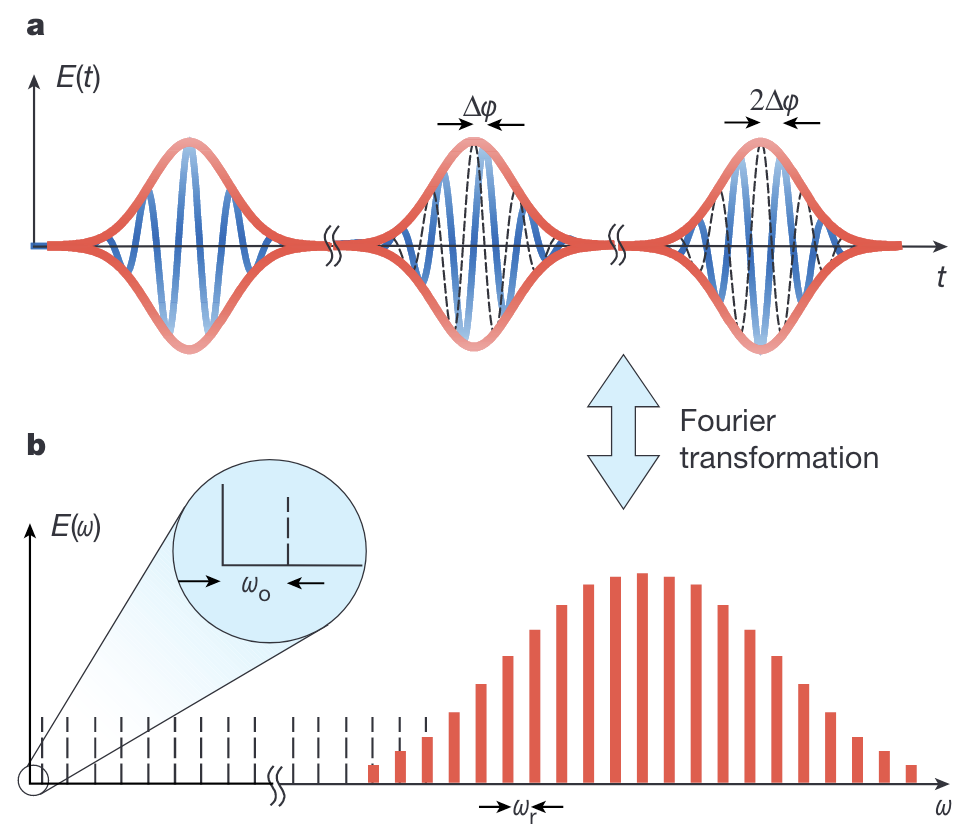
\includegraphics[width=0.7\linewidth]{figure/fig_3.png}
    \caption{光学频率梳。a.时域上为等间隔的脉冲包络,实际电场有着相位偏差。b.频域上为等间距的梳齿,在延拓到零频处有偏移。}
    \label{fig:enter-label}
\end{figure}
由于脉冲的群速度和相速度差别,光频段等间隔的谱线延伸到零频附近时会有偏移$f_{CEO}$。重复频率$f_{rep}$容易获得;通过自参考,也可测得偏移频率$f_{CEO}$。\\
由此,各模式的频率即可写为:
\[f_n = f_{CEO} + n * f_{rep}\]
$n$的量级为$10^6$。光学频率梳相干地连接了电子学和光学两个领域,催生了一系列研究:光钟,光谱探测,低噪声微波。\\
\begin{figure}[htbp]
    \centering
    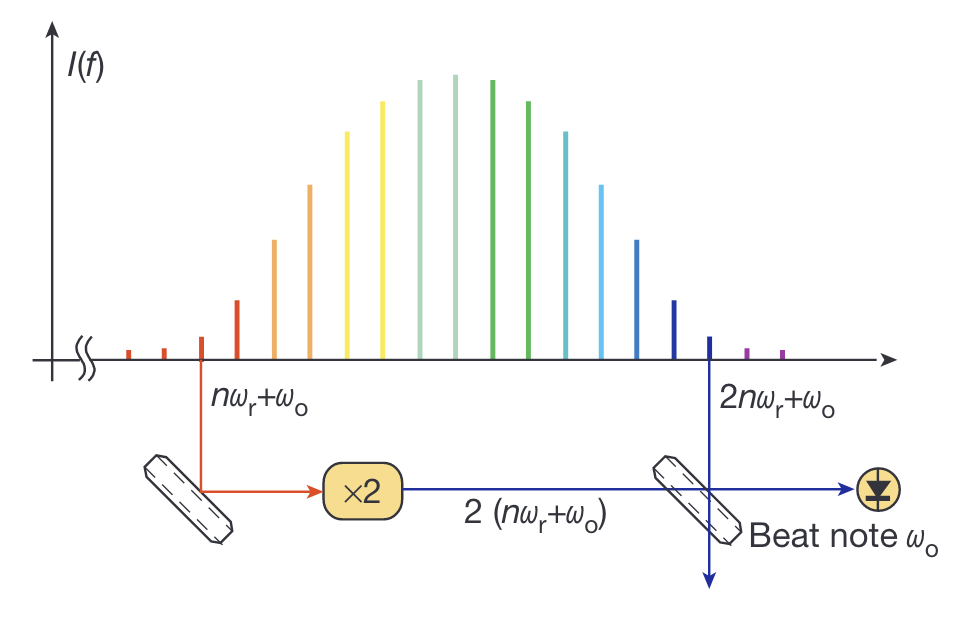
\includegraphics[width=0.7\linewidth]{figure/fig_2.png}
    \caption{自参考技术。选出跨倍频程光梳$~^{[4]}$的$n$和$2n$模式,将低频模式倍频,即可与高频模式拍出光梳的偏移频率。}
    \label{fig:enter-label}
\end{figure}
\subsection{Kerr梳}
Kerr梳利用材料的三阶非线性效应,通过简并和非简并四波混频在泵浦光两边级联产生等间距的梳尺$~^{[8]}$。对于三阶非线性,$Q^2/V$表征了非线性的强度。亮孤子态是一种锁模态,时域上是稳定的脉冲。孤子通过平衡损耗与非线性增益,色散与Kerr效应而保持稳定,存在于反常群速度色散的腔中。$~^{[10]}$\\
\begin{figure}[htbp]
    \centering
    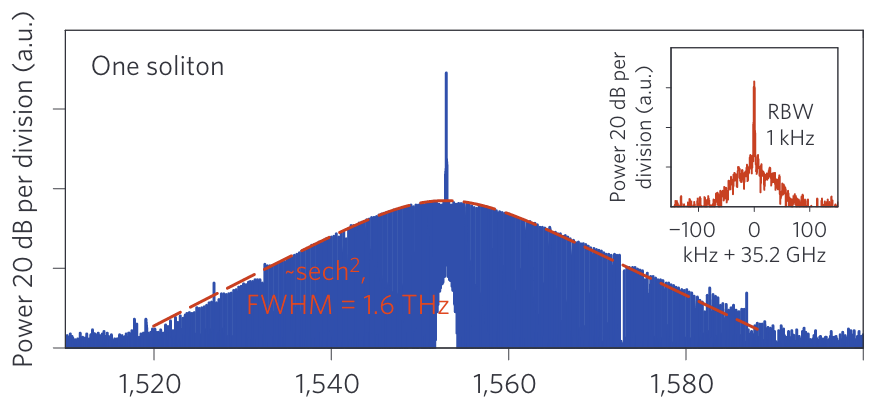
\includegraphics[width=0.7\linewidth]{figure/fig_6.png}
    \caption{单孤子态。}
    \label{fig:enter-label}
\end{figure}
进入孤子态通常需要复杂的泵浦频率或强度调节过程。
\subsection{电光梳}
电光梳通过光学回路中的相位调制器产生。泵浦光受到调制而产生边带,当调制频率与重频相等时,边带也被谐振加强且受到调制,又产生新边带,如此级联形成了电光梳。\\
\begin{figure}[htbp]
    \centering
    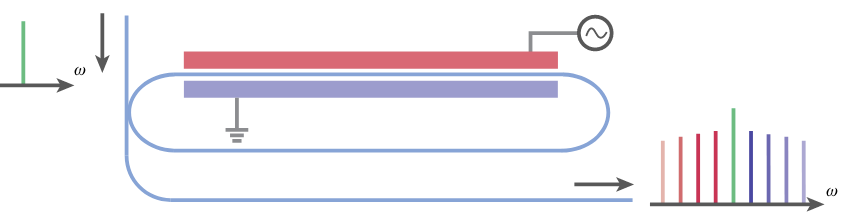
\includegraphics[width=0.7\linewidth]{figure/fig_5.png}
    \caption{电光梳。腔内谐振的电光调制将部分输入单频光转化为输出的级联边带。}
    \label{fig:enter-label}
\end{figure}
电光梳结构简单,但早期电光梳的转换效率和展宽受制于弱电光作用强度和无法控制色散。
\subsection{集成锁模激光器——研究动机}
锁模激光器是最早用来产生超短脉冲的结构。锁模激光器在稳态下,回路中也存在着孤子,并同时满足增益-损耗,色散-非线性的平衡。增益来源于受到泵浦的增益介质,非线性则是锁模的关键。早期,锁模激光器采用强度调制等主动锁模方式;如今大部分则依靠饱和吸收体等被动锁模方式运行。\\
由于集成平台上缺少成熟的引入增益介质的工艺,因此集成锁模激光器领域尚处在研究的早期阶段。
\section{铌酸锂简介}
集成光子学平台有很多:硅,氮化硅,氮化铝等等,但只有铌酸锂同时具有1.低损耗,2.高非线性,3.快速响应的电光调制。$~^{[17]}$因此铌酸锂是进行光电研究的极佳材料。铌酸锂在光纤光学中很常见:电光调制器、频率转换器等等。但由于铌酸锂难以进行微纳加工,传统的铌酸锂波导对与光场的局域性差。直到最近十年,铌酸锂平面波导工艺的突破,让铌酸锂再次成为集成光子学研究的活跃平台。
\subsection{二阶非线性效应}
铌酸锂的晶体结构为3m点群,无中心反演对称性,因此具有二阶非线性效应。\\
二阶非线性效应也叫做线性电光效应,通过Pockels矩阵描述,可以简写为:
\[\Delta \epsilon_{ij} = -\Sigma_k epsilon_{ii}\epsilon_{jj}r_{ijk}E_k/\epsilon_0\]
铌酸锂中最大的线性电光系数为$r_{333} = 31pm/V$,使用这一系数需要使得外加微波电场和光场的方向都与晶体z轴平行。
\subsection{三阶非线性效应}
铌酸锂的非线性折射率为$n_2 = 1.8*10^{-19}m^2/W$,与氮化硅$2.5*10^{-19}$为一个量级。因此也可以在铌酸锂上产生Kerr梳。
\subsection{光折变}
光折变时受激发载流子的空间不均匀分布形成的电场而在二阶非线性材料中产生的局部折射率变化。由于波导内外光强差异大,因此薄膜铌酸锂波导有着很强的光折变效应。\\
光折变产生的折射率变化方向$~^{[9]}$与热效应$~^{[3]}$相反,弛豫时间更长。两者的相互作用可使Kerr孤子自启动。
% \section{本文内容安排}
% 本文共六章节,

	\chapter{集成主动锁模激光器的构型}
\label{sec:related}

\fontsize{12bp}{14.4pt}

\section{谐振腔}
实验用样品为铒镱双掺。铒离子在$980nm$处的吸收截面较小,共同掺杂利用了镱离子在该波段处的大吸收截面,再通过振动将能量传递给周围的铒离子,以等效提升铒离子在该波段的泵浦吸收效率。\\
\begin{figure}[htbp]
    \centering
    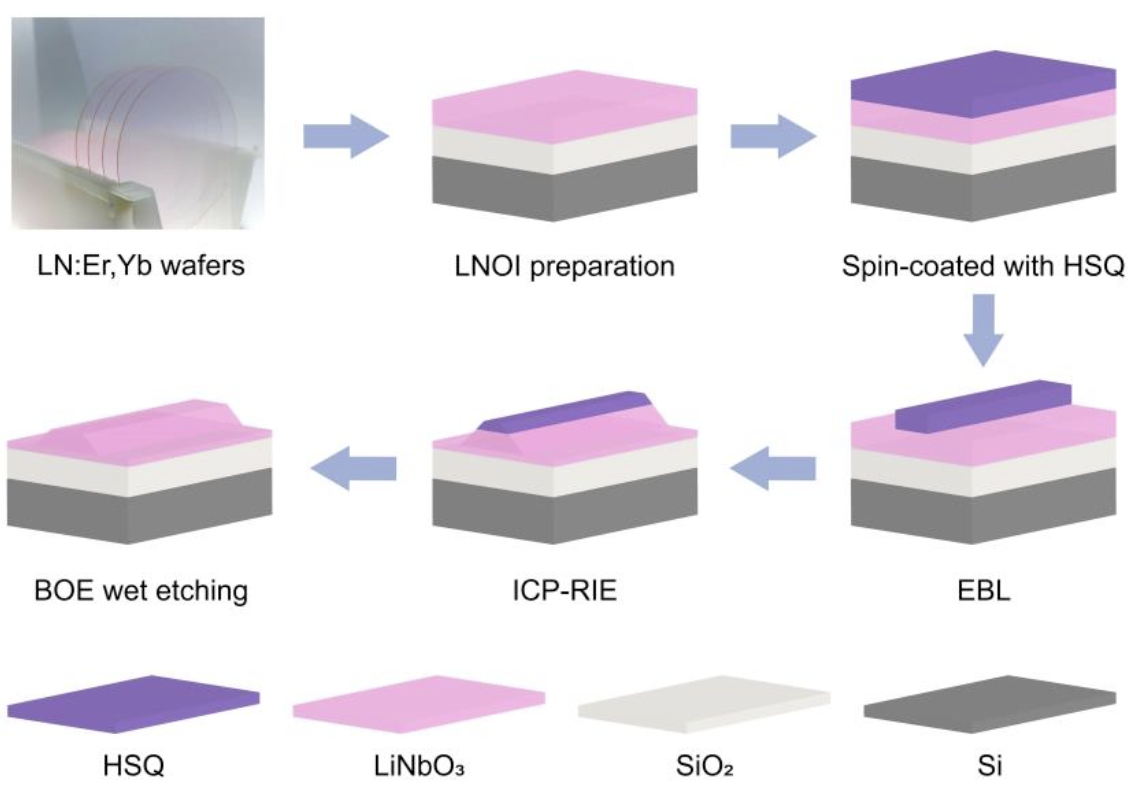
\includegraphics[width=0.7\linewidth]{figure/fig_1.png}
    \caption{铒镱双掺LNOI工艺流程}
    \label{fig:1}
\end{figure}
掺杂铌酸锂晶体通过Czochralski方法生长。再通过“smart-cut”技术制作LNOI晶圆。然后是半导体工艺:涂胶、曝光、蚀刻。
\begin{figure}[htbp]
    \centering
    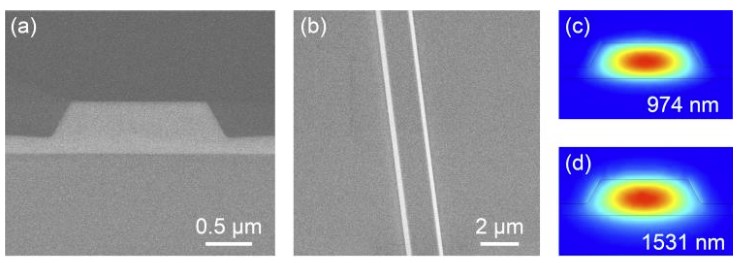
\includegraphics[width=0.7\linewidth]{figure/fig_7.png}
    \caption{a.SEM截面图。b.SEM俯视图。c,d. $974nm$和$1531nm$波长的模场分布。}
    \label{fig:enter-label}
\end{figure}
最终成品波导的厚度为$400nm$,底角为$60$度。
\begin{figure}[htbp]
    \centering
    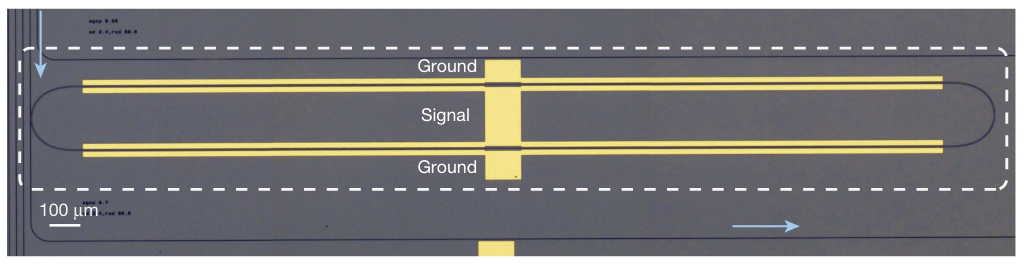
\includegraphics[width=0.95\linewidth]{figure/fig_8.png}
    \caption{波导与腔的构型图$~^{[2]}$}
    \label{fig:enter-label}
\end{figure}
为了利用最大的电光系数,腔被做成了跑道形,长边与z轴垂直。腔与外波导通过隐失波耦合。
\section{增益介质}
光信号的放大在光学中非常重要,常见的增益介质为稀土金属或III-IV族半导体。
掺铒光纤放大器在光纤通信中很成功,意味着铒离子也是集成平台上增益介质的极佳选择。$~^{[13]}$\\
使用Czochralski方法,在熔融阶段加入稀土元素,即可完成掺杂。\\
实际实验使用$1480nm$泵浦,因此仅需考虑铒离子的能级结构。$~^{[1]}$
\begin{figure}[htbp]
    \centering
    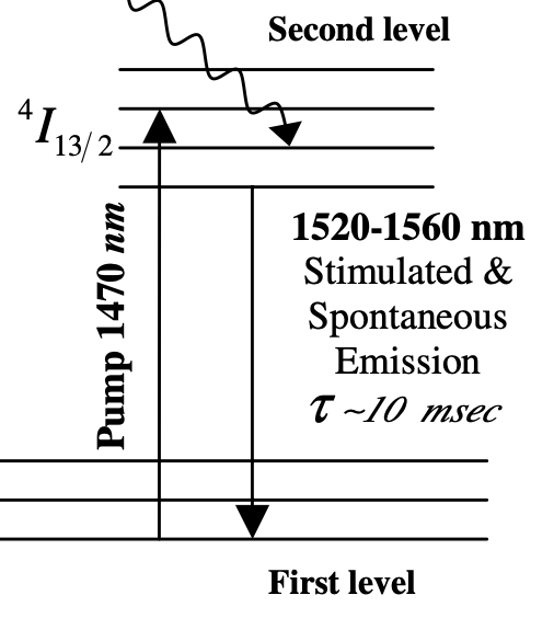
\includegraphics[width=0.5\linewidth]{figure/fig_27.png}
    \caption{铒离子的能级结构}
    \label{fig:enter-label}
\end{figure}
可用简化的三能级系统表示铒离子能级。下能级到上能级为泵浦。中间能级为一亚稳态,寿命约为$10ms$。上能级到中间能级的跃迁为无辐射跃迁,不释放或吸收光子,且速率较快。亚稳态到下能级的跃迁产生信号光。
\section{电光调制}
通过在平行于波导的两侧镀上金电极,可以在外部微波源的激励下产生面内垂直于波导方向的电场。可与TE模式光场产生最强的电光相互作用。\\
\begin{figure}[htbp]
    \centering
    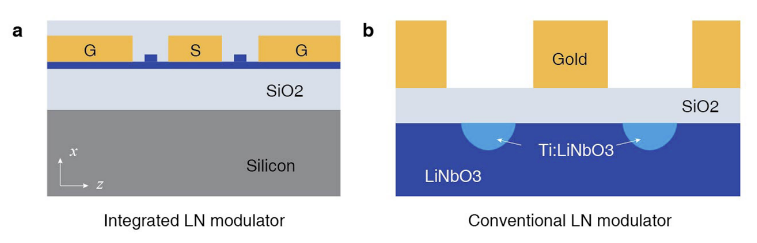
\includegraphics[width=0.8\linewidth]{figure/fig_10.png}
    \caption{带电极的波导截面图:a.强束缚波导,b.弱束缚波导}
    \label{fig:enter-label}
\end{figure}
G-S-G的电极构型充分利用了上下两段波导作为电光作用区域。通过交流探针,可将电信号施加到电极上。
	\chapter{光场的动力学方程}
\label{chap:model1}

\fontsize{12bp}{14.4pt}

\section{泵浦-增益-激射}
三能级系统中,当上中能级之间的跃迁速率远快于中下时,给予下上能级间的泵浦即可在中下之间形成粒子数反转。\\
泵浦光被消耗,将处于低能级的Er离子泵到高能级上,再迅速落入中间能级。
信号光从初始噪声中长出,消耗反转粒子数,以平衡损耗。\\
\subsection{增益介质的方程}
设三个能级上的粒子数从低能级到高能级依次为:$N_1, N_2, N_3$。\\
粒子数守恒:
\[N = N_1 + N_2 + N_3\]
三个能级间两两可以跃迁,共有三个过程。其中下能级到上能级对应泵浦光$1480nm$;
中间能级到下能级对应信号光$1530nm$;上能级到中间能级为无辐射跃迁。\\
\[\frac{dN_1}{dt} = -R_p^a N_2 + R_p^e N_3 - R_s^a N_1 + R_s^e N_2 + \frac{1}{\tau_g} N_2\]
\[\frac{dN_2}{dt} = -R_s^e N_2 + R_s^a N_1 - \frac{1}{\tau_g} N_2 + \gamma_{23} N_3\]
\[\frac{dN_3}{dt} = R_p^a N_1 - R_p^e N_3 - \gamma_{23} N_3\]
其中,$R_{p,s}^{a,e}$为各跃迁过程的速率,与增益介质的散射截面相关:
\[R_{p,s}^{a,e} = \frac{\sigma_{p,s}^{a,e} \Gamma_{p,s}}{h\nu_{p,s} A} P_{p,s}\]
无辐射跃迁的弛豫时间短,因此中间能级和上能级之间始终满足玻尔兹曼分布:
\[\beta = \frac{N_3}{N_2} = \exp{(-\frac{\Delta E}{k_B T})}\]
利用粒子数守恒和上中能级间的关系,可以用$N,N_1$表示粒子数。
\[N_2 = \frac{1 - N_1/N}{1+\beta} N,\ N_3 = \frac{\beta(1 - N_1/N)}{1+\beta} N\]
因此,三个能级的速率方程只剩下一个有效,不妨选用$N_1$:
\[\frac{dN_1}{dt} = -\frac{1}{\tau_{N_1}} (N_1 - N_{eq})\]
\subsection{光场的方程}
腔中前后两个方向的传播模式没有区别,必须同时考虑。\\
光受到的增益为:
\[\frac{d P_{p,s}^{\pm}}{dz} = \pm \Gamma_{p,s} (\sigma_{p,s}^e N_{3,2} - \sigma_{p,s}^a N_1) P_{p,s}^{\pm} \mp \alpha_0 P_{p,s}^{\pm}\]
其中$\alpha_0$为传输损耗
设信号光电场的增益为$g$,小信号增益为$g_0$:
\[g = \frac{1}{2} \Gamma_s L_d (\sigma_s^eN_2 - \sigma_s^a N_1)\]
平衡态的增益应当具有饱和的形式,而非平衡时则会弛豫到平衡,因此猜测增益的演化方程为:
\[\tau^\prime \frac{dg}{dt} = g_0 - (1+\frac{P_s}{P_{sat}}) g\]
带入之前的方程组可得:
\[\frac{1}{\tau^\prime} = \frac{1}{1+\beta} [\frac{1}{\tau_g} + (1+\beta+\beta \frac{\sigma_p^e}{\sigma_p^a})R_p^a]\]
\[P_{sat} = \frac{h \nu_s A}{\Gamma_s \tau^\prime (\sigma_s^a + \frac{1}{1+\beta}\sigma_s^e)}\]
\[g_0 = \frac{1}{2} \Gamma_s L_d \sigma_s^e N \frac{\tau^\prime}{1 + \beta} [(1 - \frac{\sigma_s^a}{\sigma_s^e} \frac{\sigma_p^e}{\sigma_p^a} \beta) R_p^a - \frac{\sigma_s^a}{\sigma_s^e} \frac{1}{\tau_g}]\]
$R_p^a$正比于泵浦光功率,因此平衡速率、信号光饱和功率正比于泵浦光功率。\\
而小信号增益$g_0$在泵浦光功率足够大时存在饱和:\\
\[g_{0,max} = \frac{1}{2} \Gamma_s L_d N \frac{\sigma_p^a \sigma_s^e - \sigma_s^a \sigma_p^e \beta}{\sigma_p^a + \beta \sigma_p^a + \beta \sigma_p^e}\]
同理可得泵浦光受到的增益:
\[g_p = \frac{1}{2} \Gamma_p L_d N \frac{\beta \sigma_p^e \sigma_s^a - \sigma_p^a \sigma_s^e}{\sigma_s^e + \sigma_s^a (1 + \beta)} + \frac{\sigma_p^e \beta + \sigma_p^a (1 + \beta)}{\sigma_s^e + \sigma_s^a (1 + \beta)} g\]
由于泵浦光波段吸收截面大于发射截面,信号光波段吸收截面小于发射截面,因此$g_p < 0$,增益介质对泵浦光实则表现为吸收。\\
\subsection{放大的自发辐射}
除了受激辐射外,增益介质中的自发辐射也被放大,表现为噪声。\\
放大自发辐射的演化方程为$~^{[7]}$:
\[\frac{d P_{ASE}}{dz} = \Gamma_s(\sigma_s^e N_2 - \sigma_s^a N_1) P_{ASE} + 2h\nu_s \Delta \nu \sigma_s^e \Gamma_s N_2 - \alpha_0 P_{ASE}\]
用只含有$g$的方程表达:
\[\frac{d P_{ASE}}{dz} = \frac{2g}{L_d} P_{ASE} + 2h\nu_s \Delta \nu \sigma_s^e \Gamma_s N_2 - \alpha_0 P_{ASE}\]
\[N_2 = \frac{N + 2g / (\Gamma_s \sigma_s^a L_d)}{1 + \beta + \sigma_s^e / \sigma_s^a}\]
带入初始值0,解得单周期ASE功率$P_{ASE0}$:
\[P_{ASE0} = h\nu_s \Delta \nu \sigma_s^e \Gamma_s N_2 L_d \frac{e^{2g} - 1}{g - l}\]
自发辐射具有相位随机性,因此单周期ASE将在加上随机相位后合并到信号光中。
\[A(0^+) = \mathcal{F}^{-1}[\mathcal{F}[A(0^-)] + \sqrt{P_{ASE}}e^{i\phi_i}]\]
\section{电光调制}
在电极上施加谐振频率的微波后,由于铌酸锂的二阶非线性效应,材料的有效折射率发生改变,相当于腔长随着时间变化,周期与脉冲周期相同。
\subsection{泵浦光--电光梳}
稳态下,泵浦光受到本征损耗和来自增益体系的稳定吸收,视作等效损耗。又受到电光调制,并且没有增益。因此泵浦光展开为电光梳。\\
电光梳的输出光场可通过简单的线性叠加获得:
\[E_{out}(t) = \sqrt{(1-\gamma)(1-k)} E_{in}(t) - k\sqrt{\frac{1-\gamma}{1-k}} \Sigma_{n=1}^{\infty}r^n e^{iMF_n(\omega_m t) E_{in}(t-nT)}\]
其中$\gamma$为输入输出耦合器插耗,$k$为其功率透过率,$r=\sqrt{\alpha(1-\gamma)(1-k)}$为单周期透过率,$1-\alpha$为单周期功率损耗比例。\\
谐振条件下:
\[F_n(\omega_m t) = \Sigma_{n=1}^{\infty} \mathrm{sin}\omega_m(t-iT)\]
\[E_{out}(t) = \sqrt{(1-\gamma)(1-k)} \hat{E_{in}}e^{i\omega_0 t} - k\sqrt{\frac{1-\gamma}{1-k}} \frac{r e^{iMsin\omega_m t}}{1-r e^{iMsin\omega_m t}} \hat{E_{in}}e^{i\omega_0 t}\]
对于泵浦光,设吸收效率为$\eta$,则有:
\[P_0 = (1-\gamma)(1-k)P_{in} |1-\frac{k}{1-k}\Sigma_{n=1}^{\infty}r^n J_0(nM)|^2\]
\[\eta = |\frac{1-k-k\Sigma_{n=1}^{\infty}r^n J_0(nM)}{1-k-k\frac{r}{1-r}}|^2\]
\begin{figure}[htbp]
    \centering
    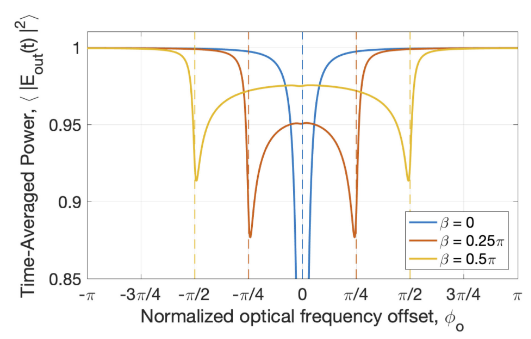
\includegraphics[width=0.8\linewidth]{figure/fig_11.png}
    \caption{不同调制深度下的谐振峰透过谱}
    \label{fig:enter-label}
\end{figure}
泵浦吸收效率$\eta$没有简约的数学表达式。
\subsection{信号光--锁模激光器}
稳态下,信号光受到本征损耗和增益,受到电光调制,形成主动锁模激光器。\\
信号光的演化由Haus方程描述:
\[T_R \frac{\partial A}{\partial T} = (-l + g(\omega) + i\delta |A|^2 - iD\frac{\partial^2}{\partial t^2} + iM\mathrm{cos}\omega_m t) A \]
有限的增益带宽:
\[g(\omega) = \frac{g}{1+(\omega - \omega_s)^2/\Omega_g^2}\]
小量近似,可将Haus方程进一步展开:
\[T_R \frac{\partial A}{\partial T} = (-l + g + i\delta |A|^2 + (iD + \frac{g}{\Omega_g^2})\frac{\partial^2}{\partial t^2} + iM(1 - \frac{1}{2} \omega_m^2 t^2))) A \]
稳态方程没有解析解,但在一定的参数条件下,可以做适当的近似使其分别可解。\\
当忽略Kerr效应时,方程变为薛定谔方程:\\
\[[(iD + \frac{g}{\Omega_g^2}) \frac{\partial^2}{\partial t^2} - iM(1 - \cos(\Omega t))] A = (l - iM - g + \lambda) A\]
对于宽度远小于谐振腔长的脉冲,可以对势能场在0点附近进行小量展开,由此得到一谐振子势场:\\
\[[(iD + \frac{g}{\Omega_g^2}) \frac{\partial^2}{\partial t^2} - iM(\frac{1}{2} \Omega^2 t^2)] A = (l - iM - g + \lambda) A\]
解为:\\
\[A_n(t) = \sqrt{\frac{W_n}{2^n \sqrt{\pi} n! \tau}} H_n(\frac{t}{\tau}) e^{-t^2 / 2\tau^2}\]
其中:\\
\[\tau = {(\frac{iD + g/\Omega^2}{iM\Omega^2/2})}^{1/4}\]
对应的本征值为:\\
\[\lambda_n = g - l + iM - iM\Omega^2 \tau^2 (n + \frac{1}{2})\]
则原薛定谔方程的解为:\\
\[A_n(T, t) = A_n(t) e^{\lambda_n T / T_R}\]
对于稳态解,要求$Re(\lambda_n) = 0$,对于一个单脉冲的产生,则对应$Re(\lambda_0) = 0$,即有:\\
\[A_0(t) = \sqrt{\frac{W_0}{\sqrt{\pi} \tau}} e^{-t^2 / 2\tau^2}\]
\[g - l = \sqrt{\frac{1}{2} M \Omega^2} {(D^2 + g^2 / \Omega^4)}^{1/4} \sin(\frac{1}{2} \arctan{(g / D\Omega^2)})\]
上述方程为腔中的增益损耗平衡关系。不同于CW态下$g = l$的平衡,此处额外引入的项来自于电光调制将能量分配到边带而带来的损耗。\\
对于实验用期间,存在关系$g >> D\Omega^2$和$g - l << l$,因此还可以进一步化简:\\
\[g - l = \frac{1}{2}\sqrt{l M} \]
此平衡关系限定了腔内铒离子增益、总损耗、电光调制深度三者的关系,否则不存在强度稳定的解。实际上,铒离子增益的可饱和性放松了这一关系。
若小信号增益为$g_0$,则稳态下的增益为:
\[g = \frac{g_0}{1 + P_s / P_{sat}}\]
由此也可以获得信号光功率的表达式:\\
\[P_s = P_{sat} (\frac{g_0}{l + \frac{1}{2} \sqrt{lM}} - 1)\]

\section{数值仿真模型}
1.根据上周期结束的状态,计算新的信号光增益和泵浦光损耗。\\
2.用电光梳模型演化泵浦光\\
3.用Haus方程演化信号光\\
4.演化ASE\\
5.将ASE合并入信号光\\
\section{本章小结}
本章给出了数值仿真的结构以及所有方程:铒离子的增益,泵浦光的电光梳形式演化方程,信号光的锁模激光器形式演化方程。在解析解方面,给出了弱输出时的腔内信号光波形和功率的解析表达式。

	\chapter{仿真结果}
\label{chap:model2}

\fontsize{12bp}{14.4pt}

\section{锁模的条件}
\subsection{调制深度}
以$FSR = 25GHz$,泵浦功率$P_{in} = 100mW$,改变调制深度进行仿真。\\
随着调制深度的增加,系统的稳态经历了混沌,周期性振荡,双脉冲,单脉冲振荡,单脉冲五个阶段。
\begin{figure}[htbp]
    \centering
    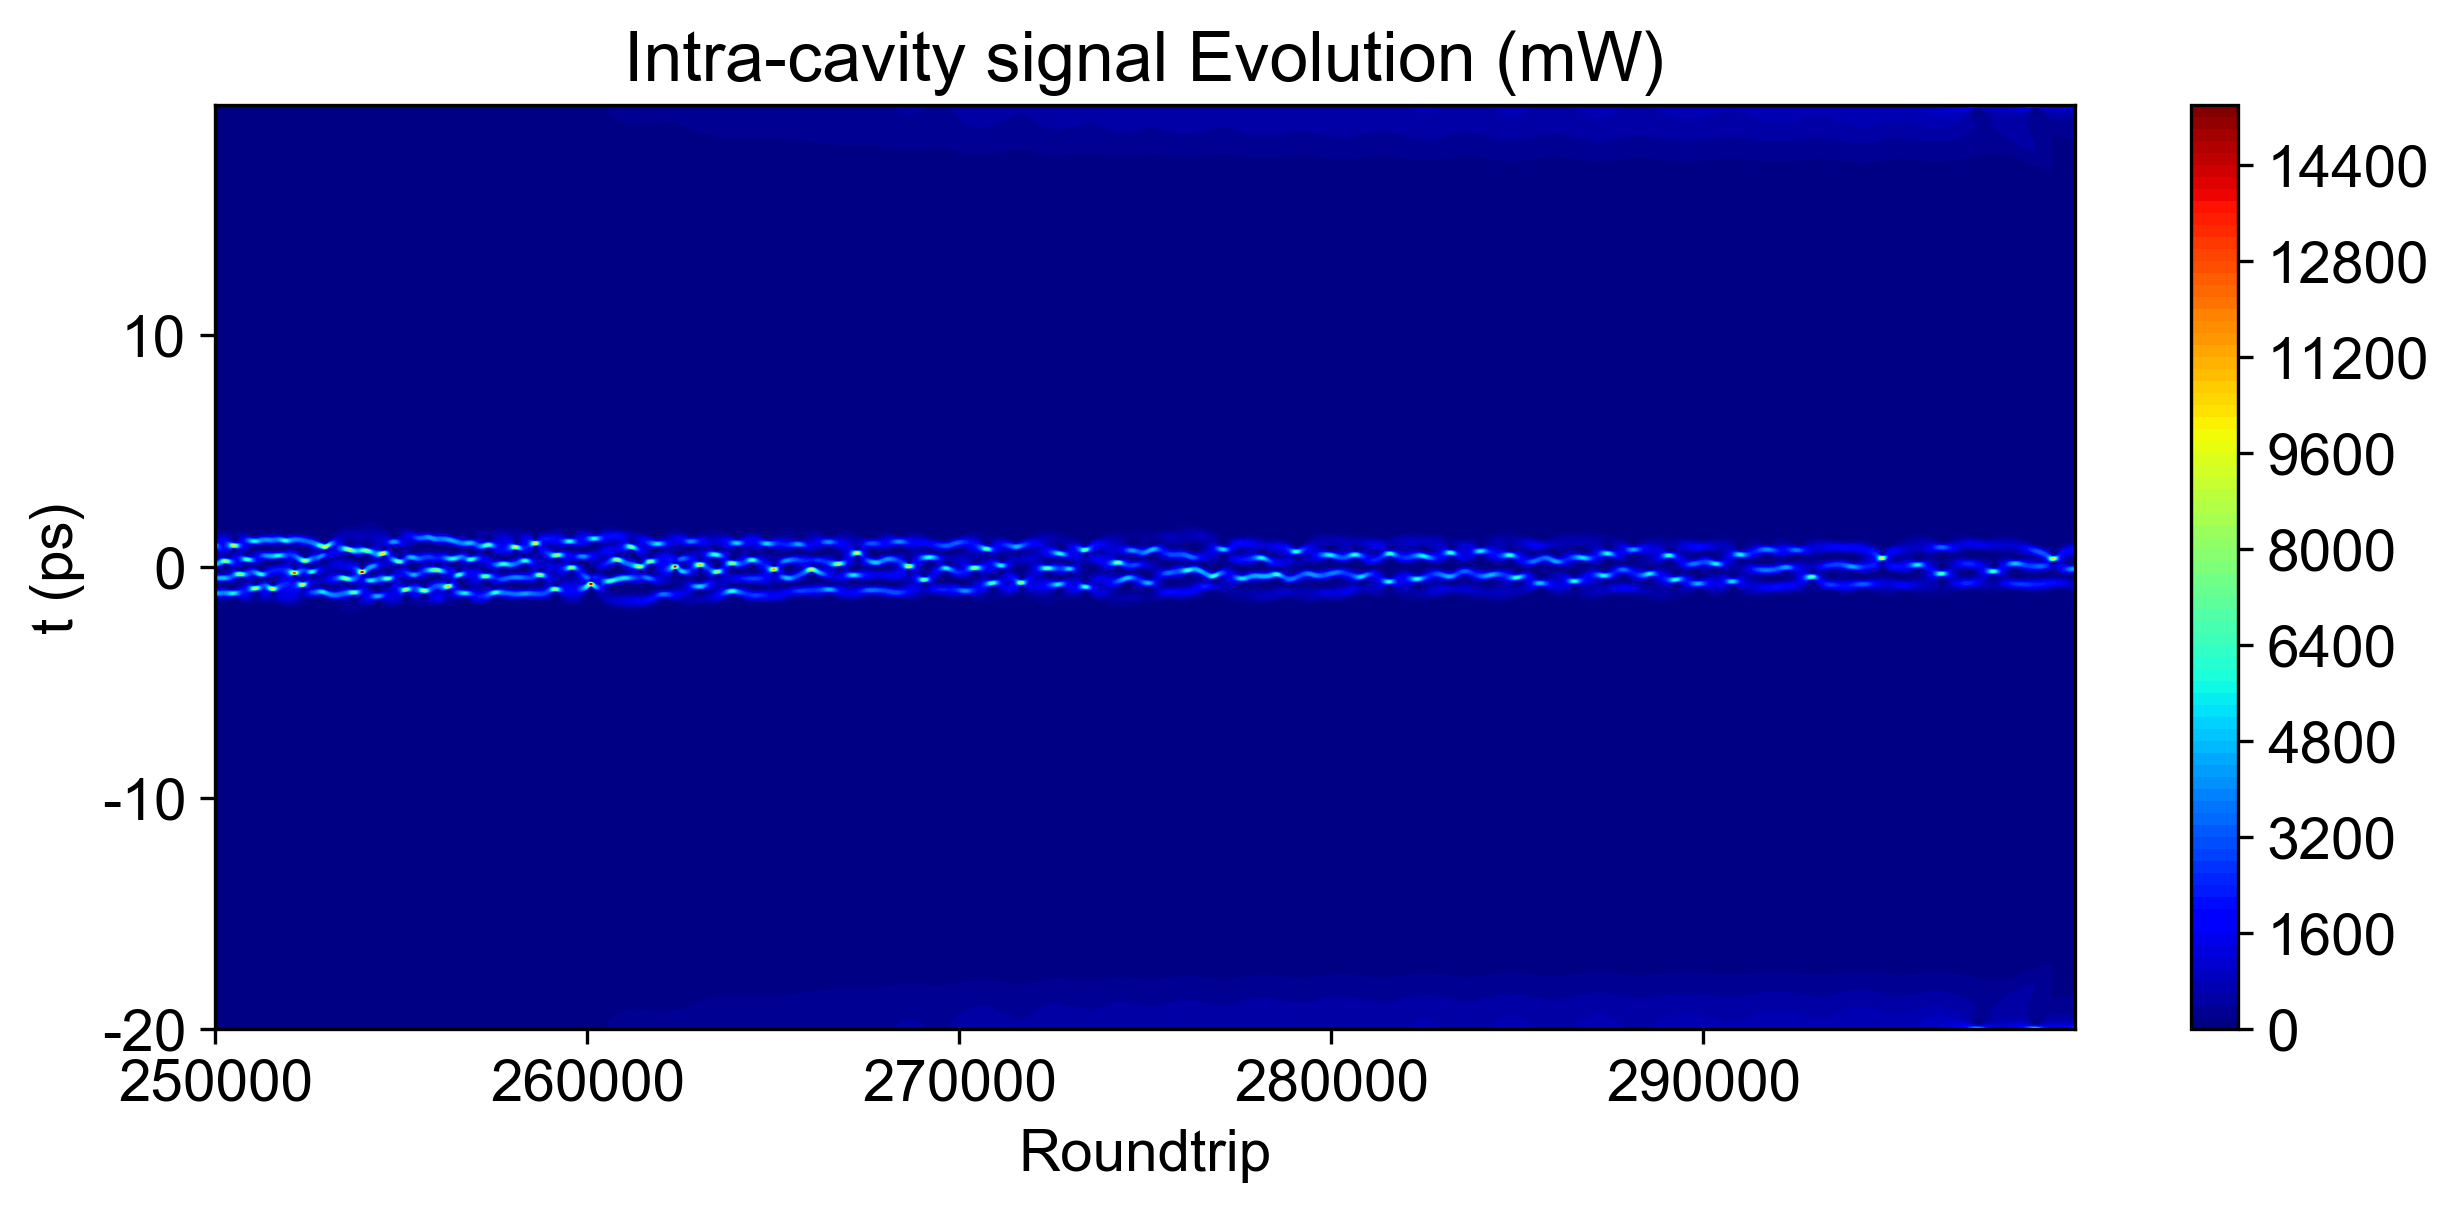
\includegraphics[width=0.48\linewidth]{figure/fig_12.png}
    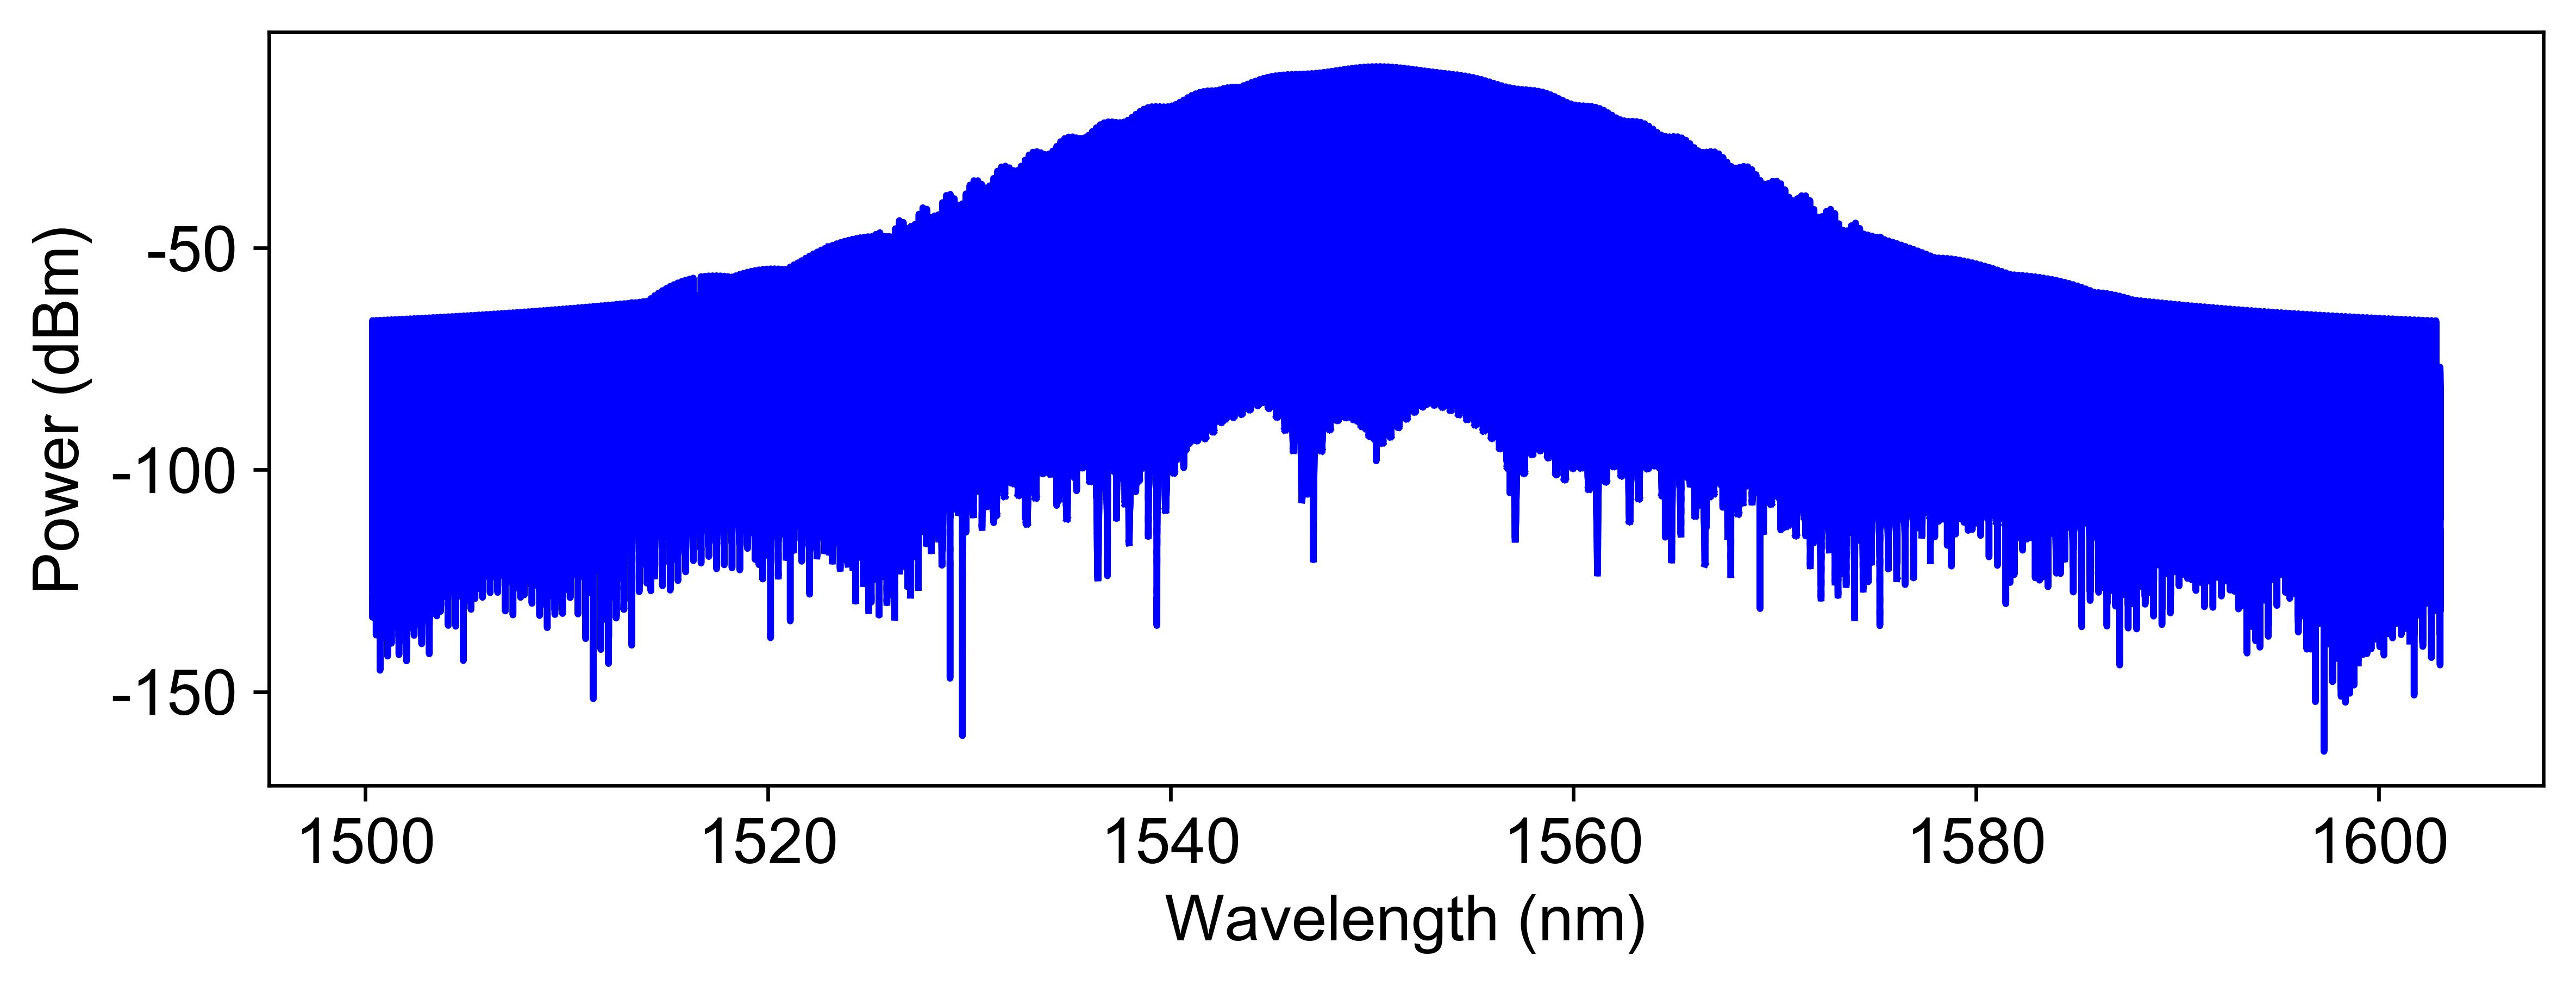
\includegraphics[width=0.48\linewidth]{figure/fig_12_0.png}
    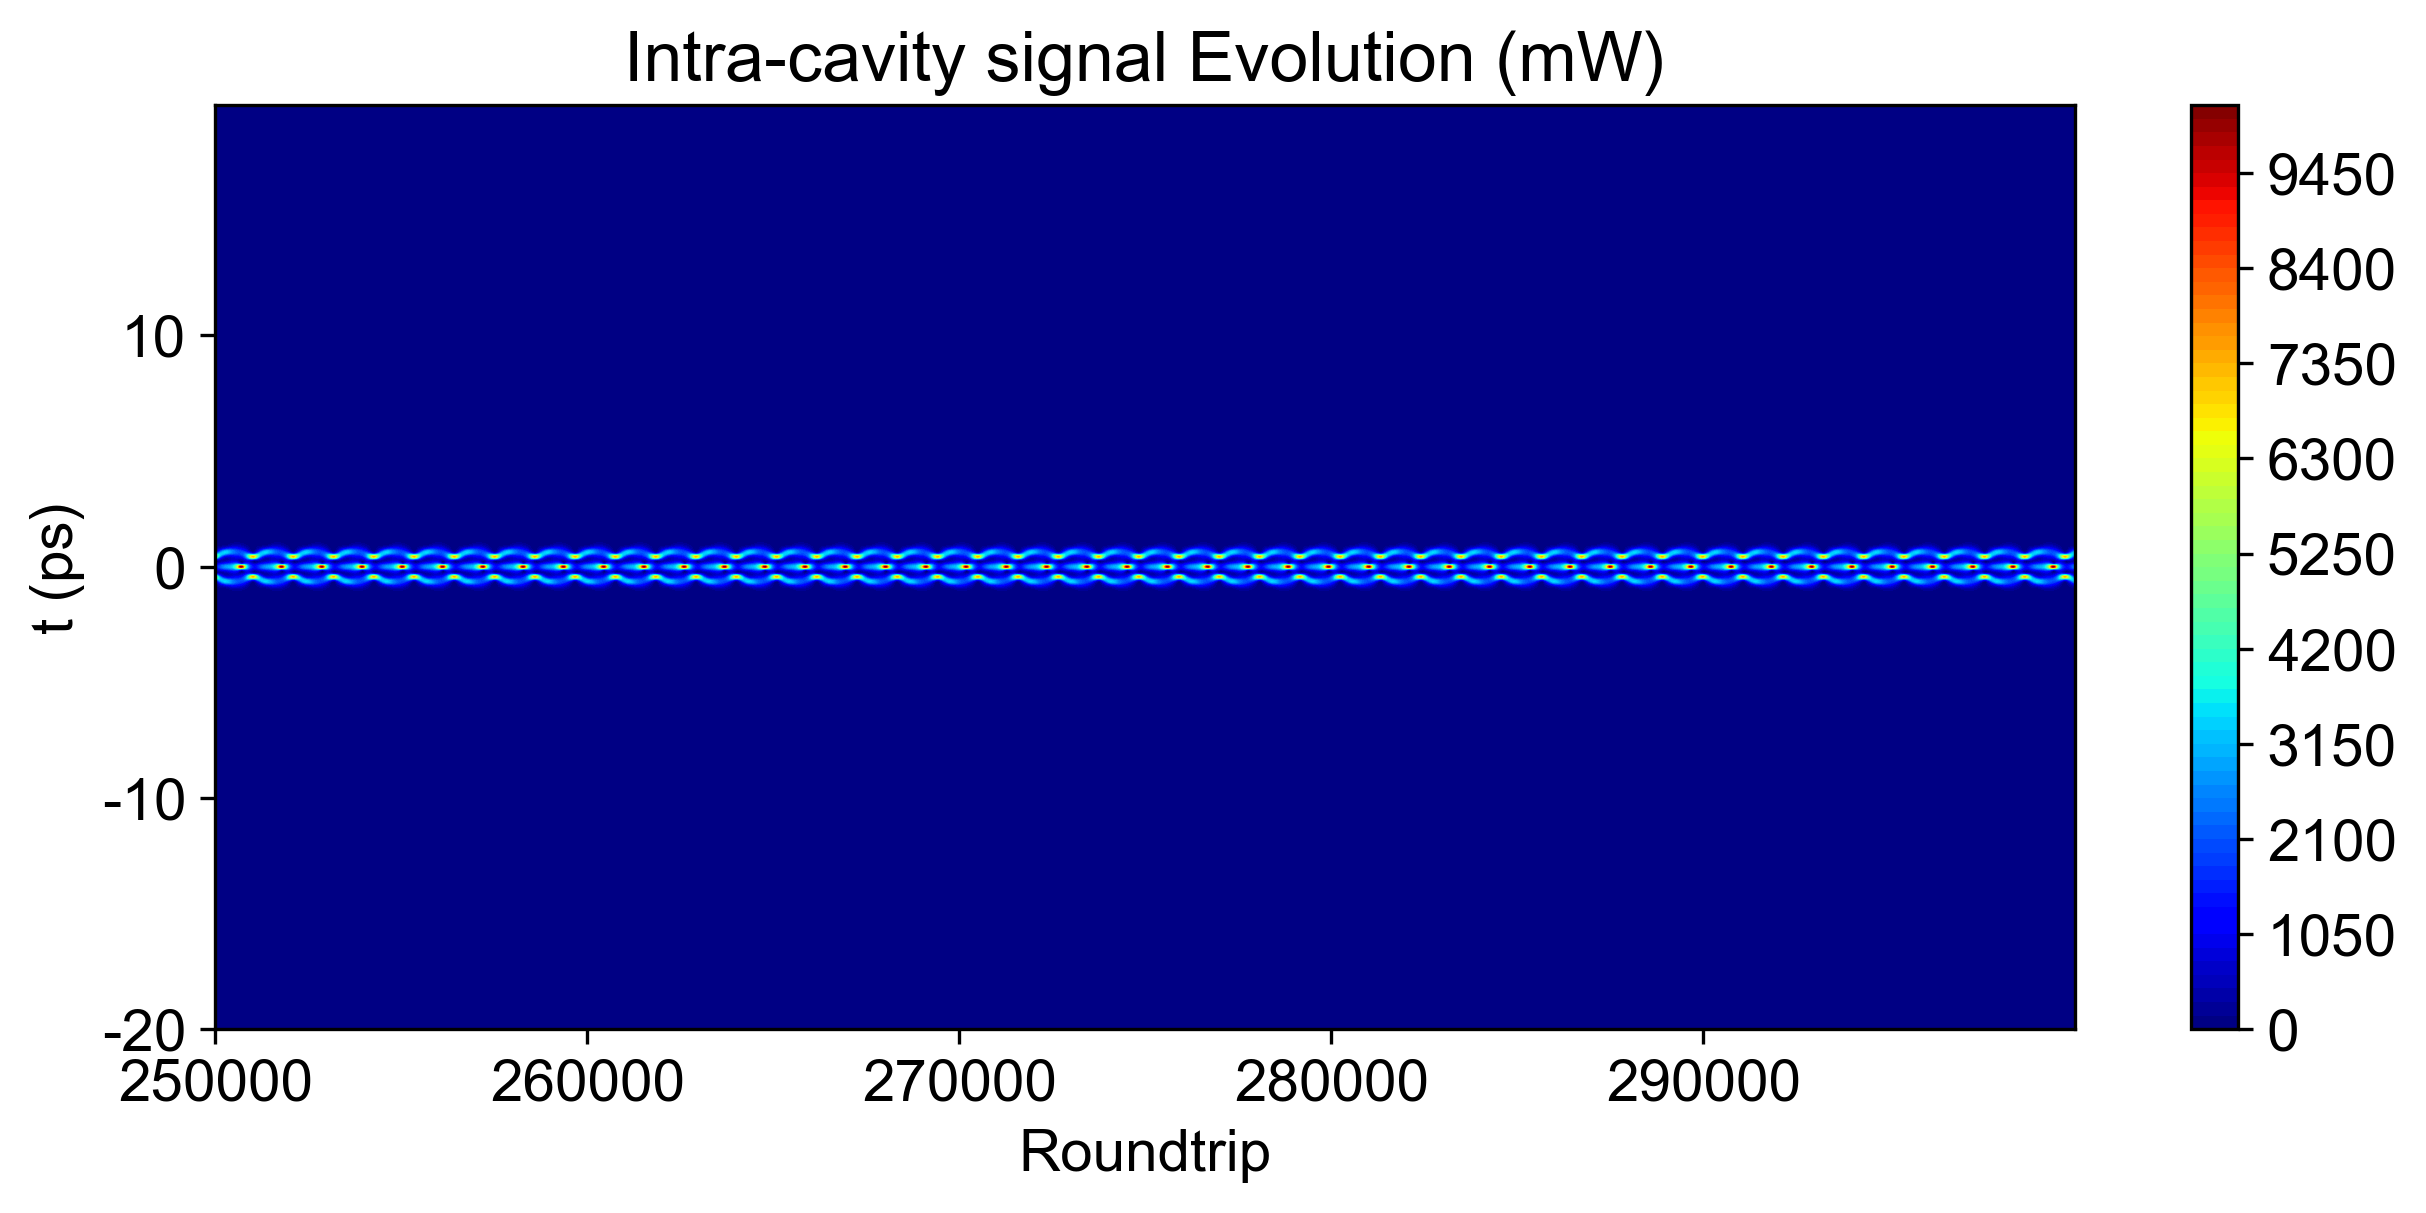
\includegraphics[width=0.48\linewidth]{figure/fig_13.png}
    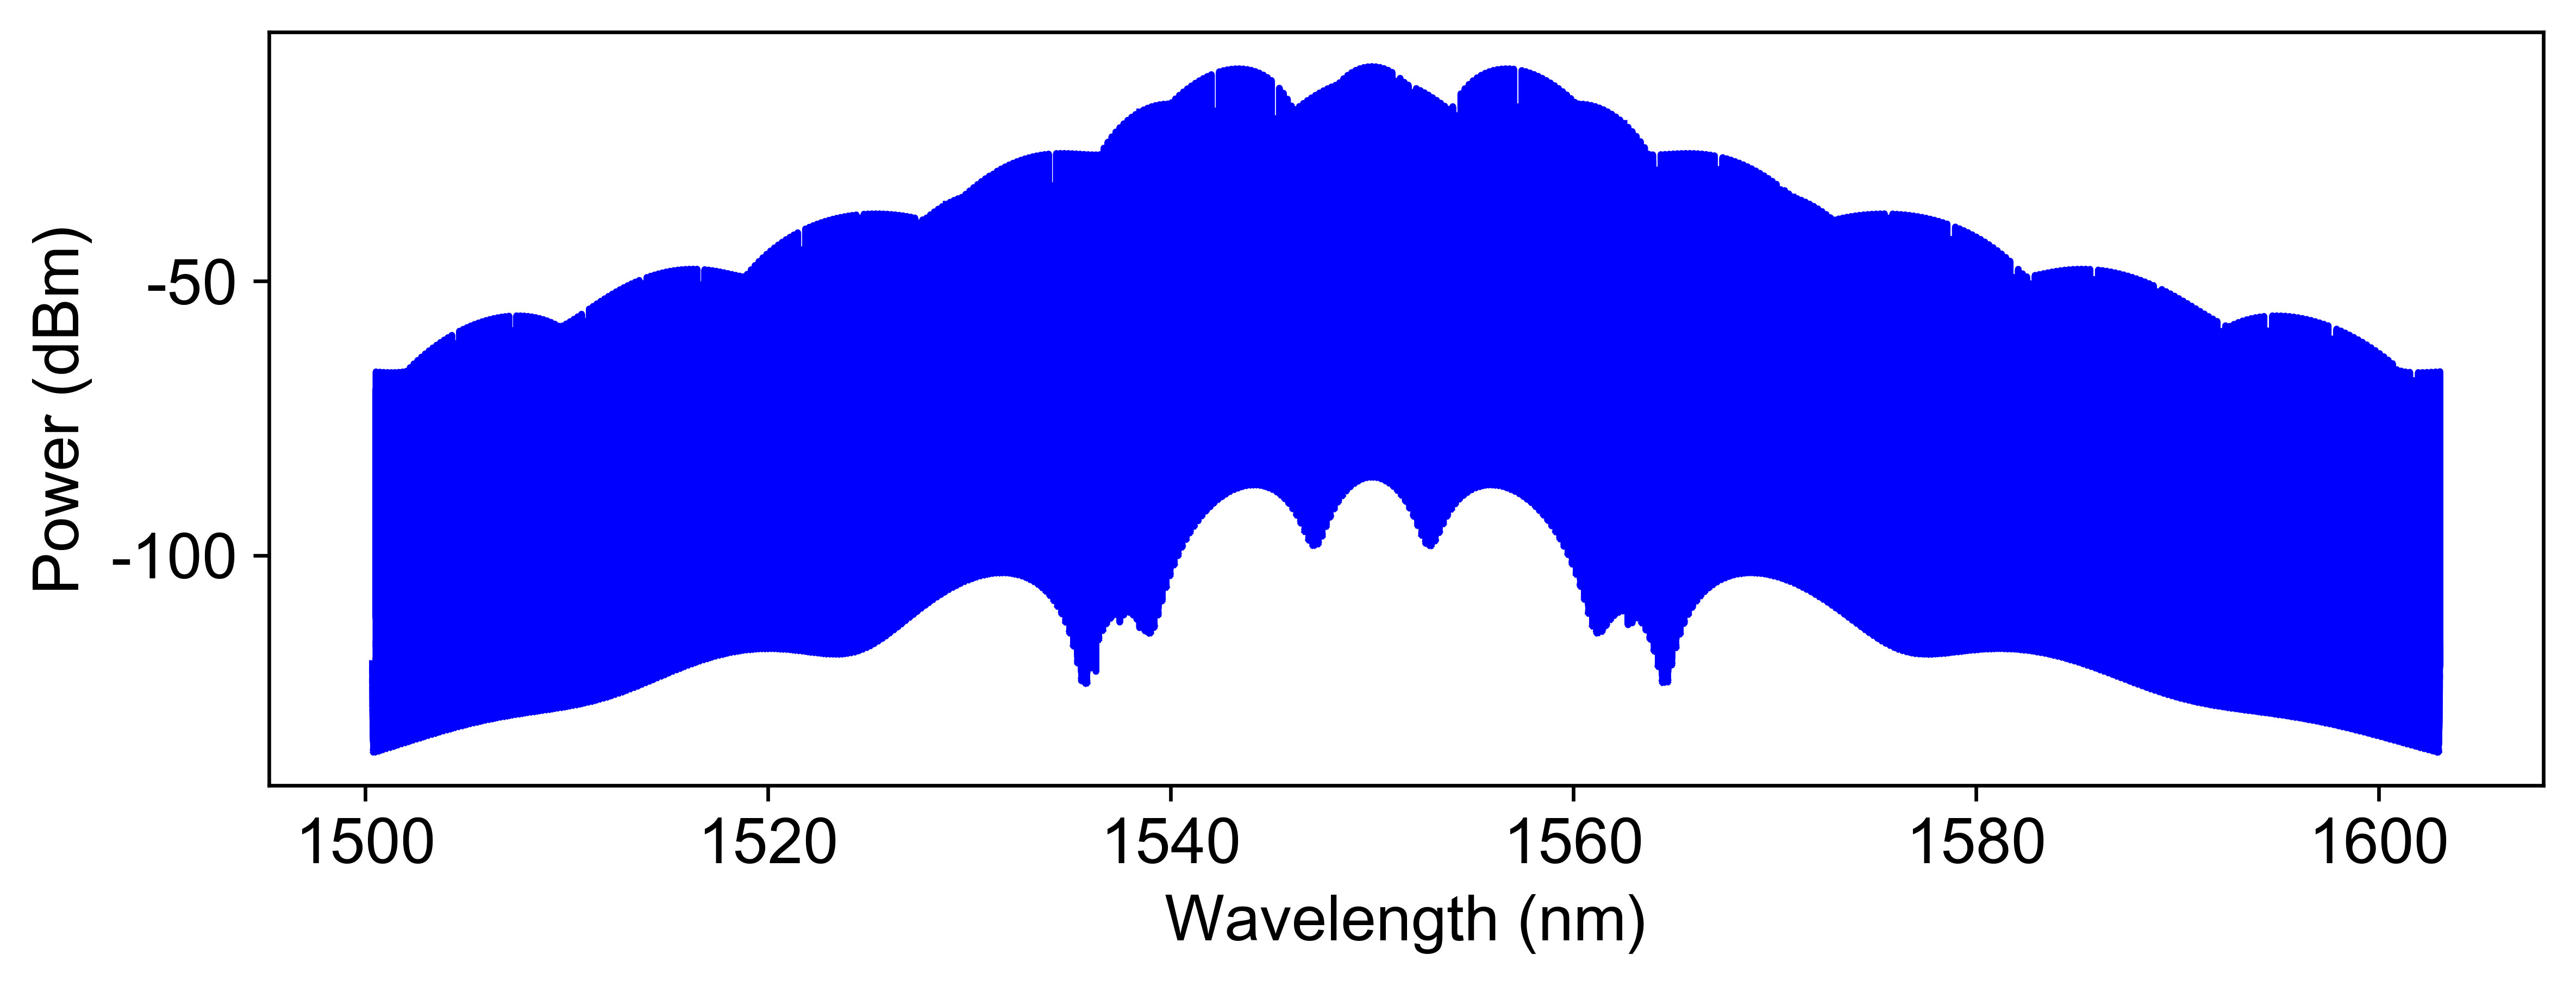
\includegraphics[width=0.48\linewidth]{figure/fig_13_0.png}
    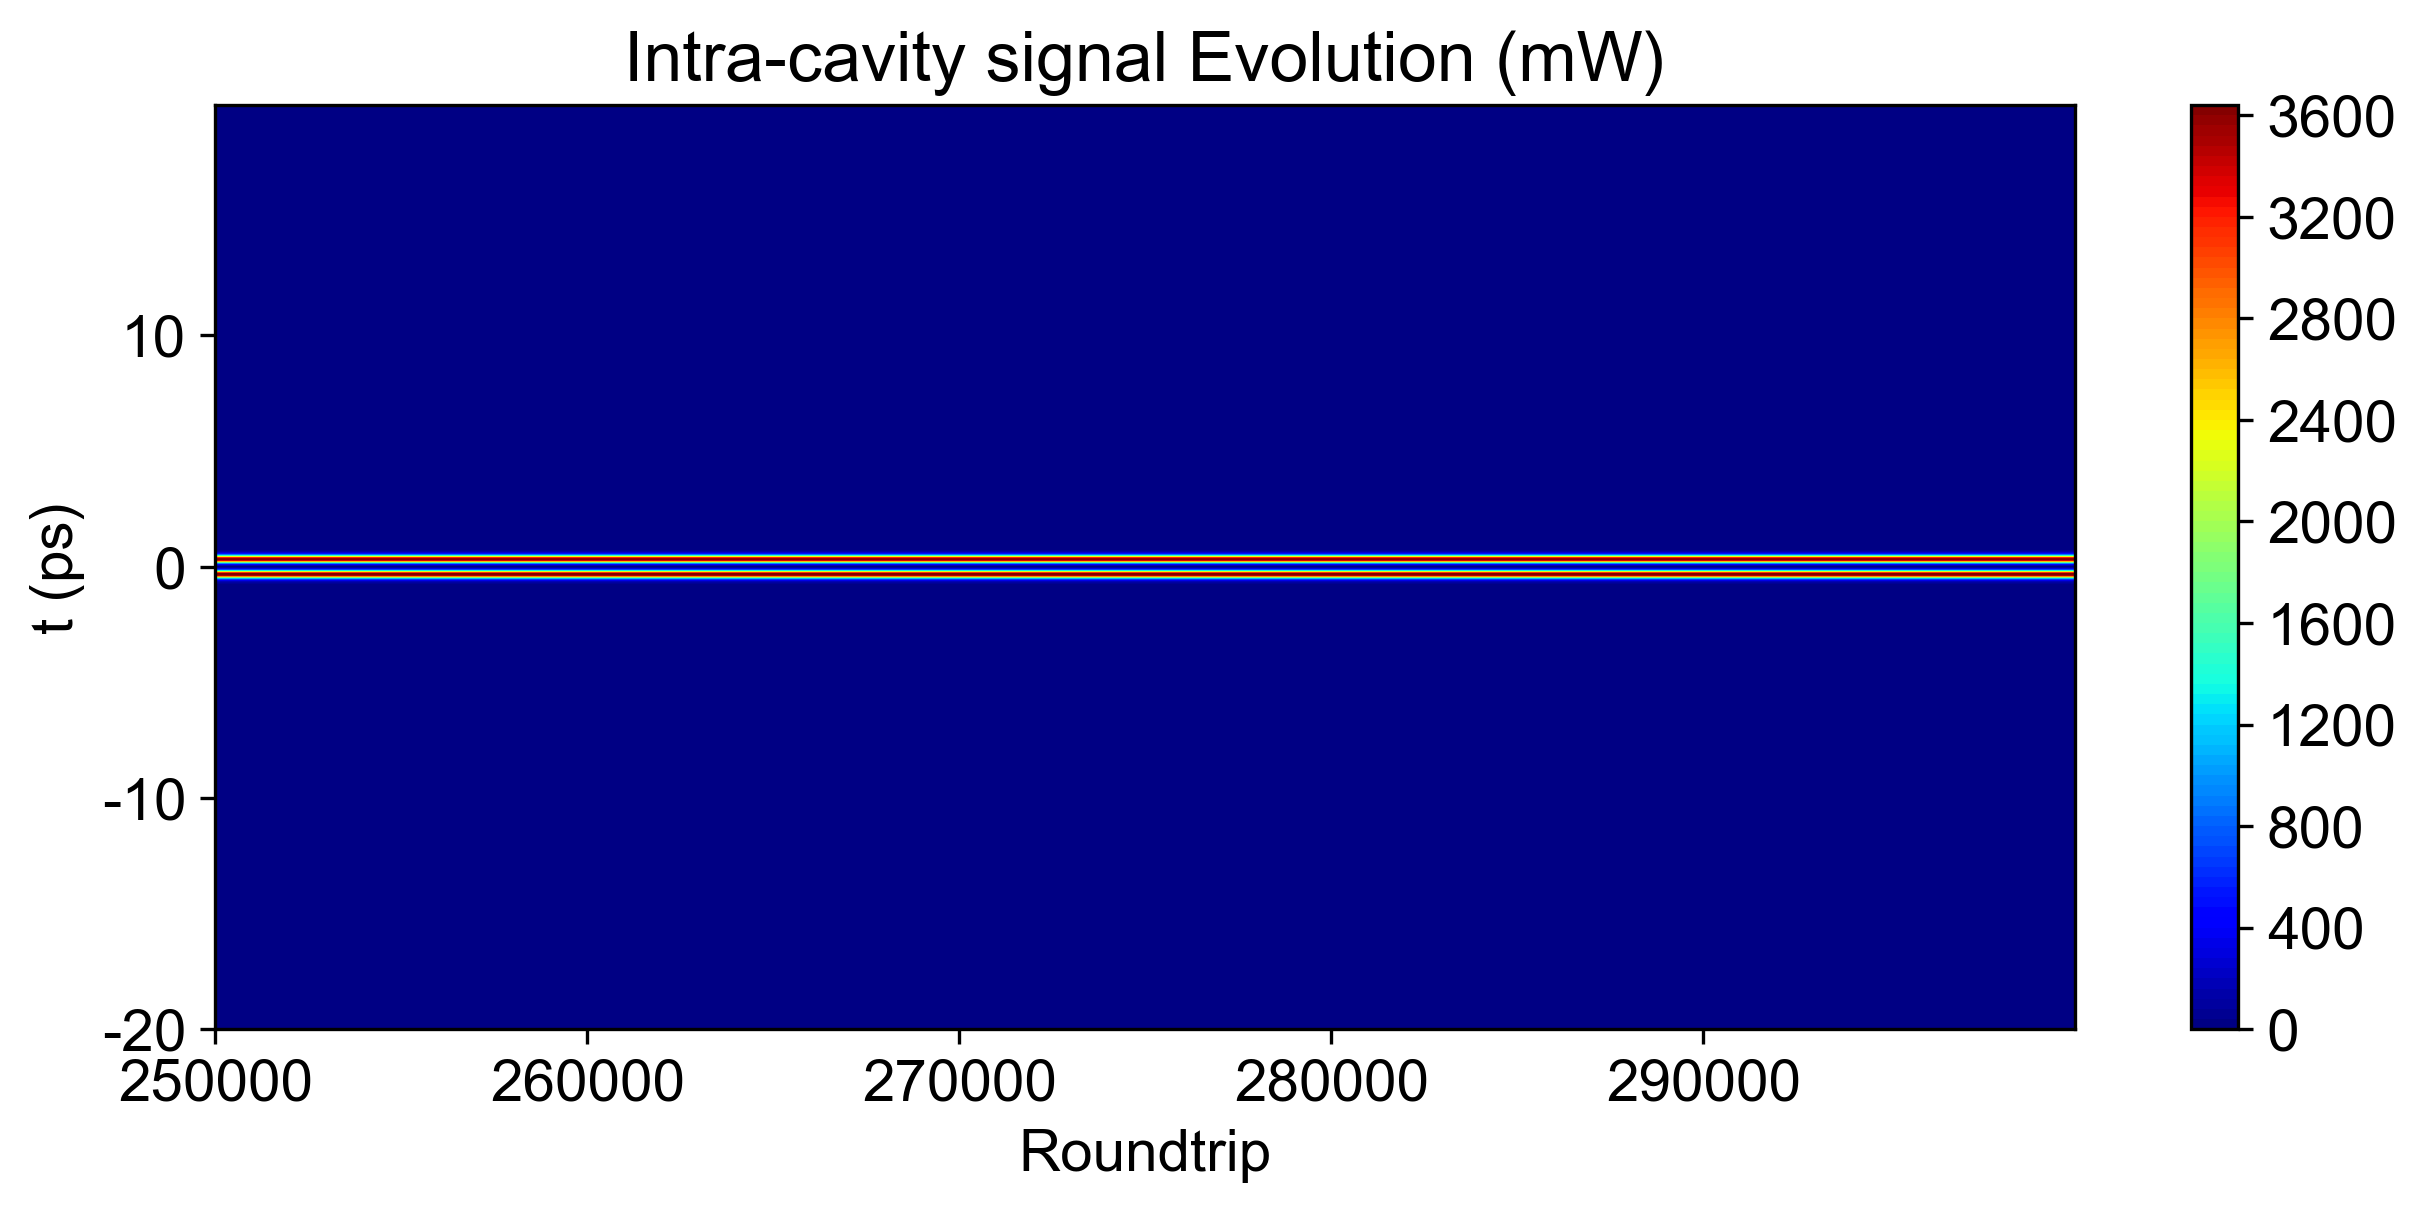
\includegraphics[width=0.48\linewidth]{figure/fig_14.png}
    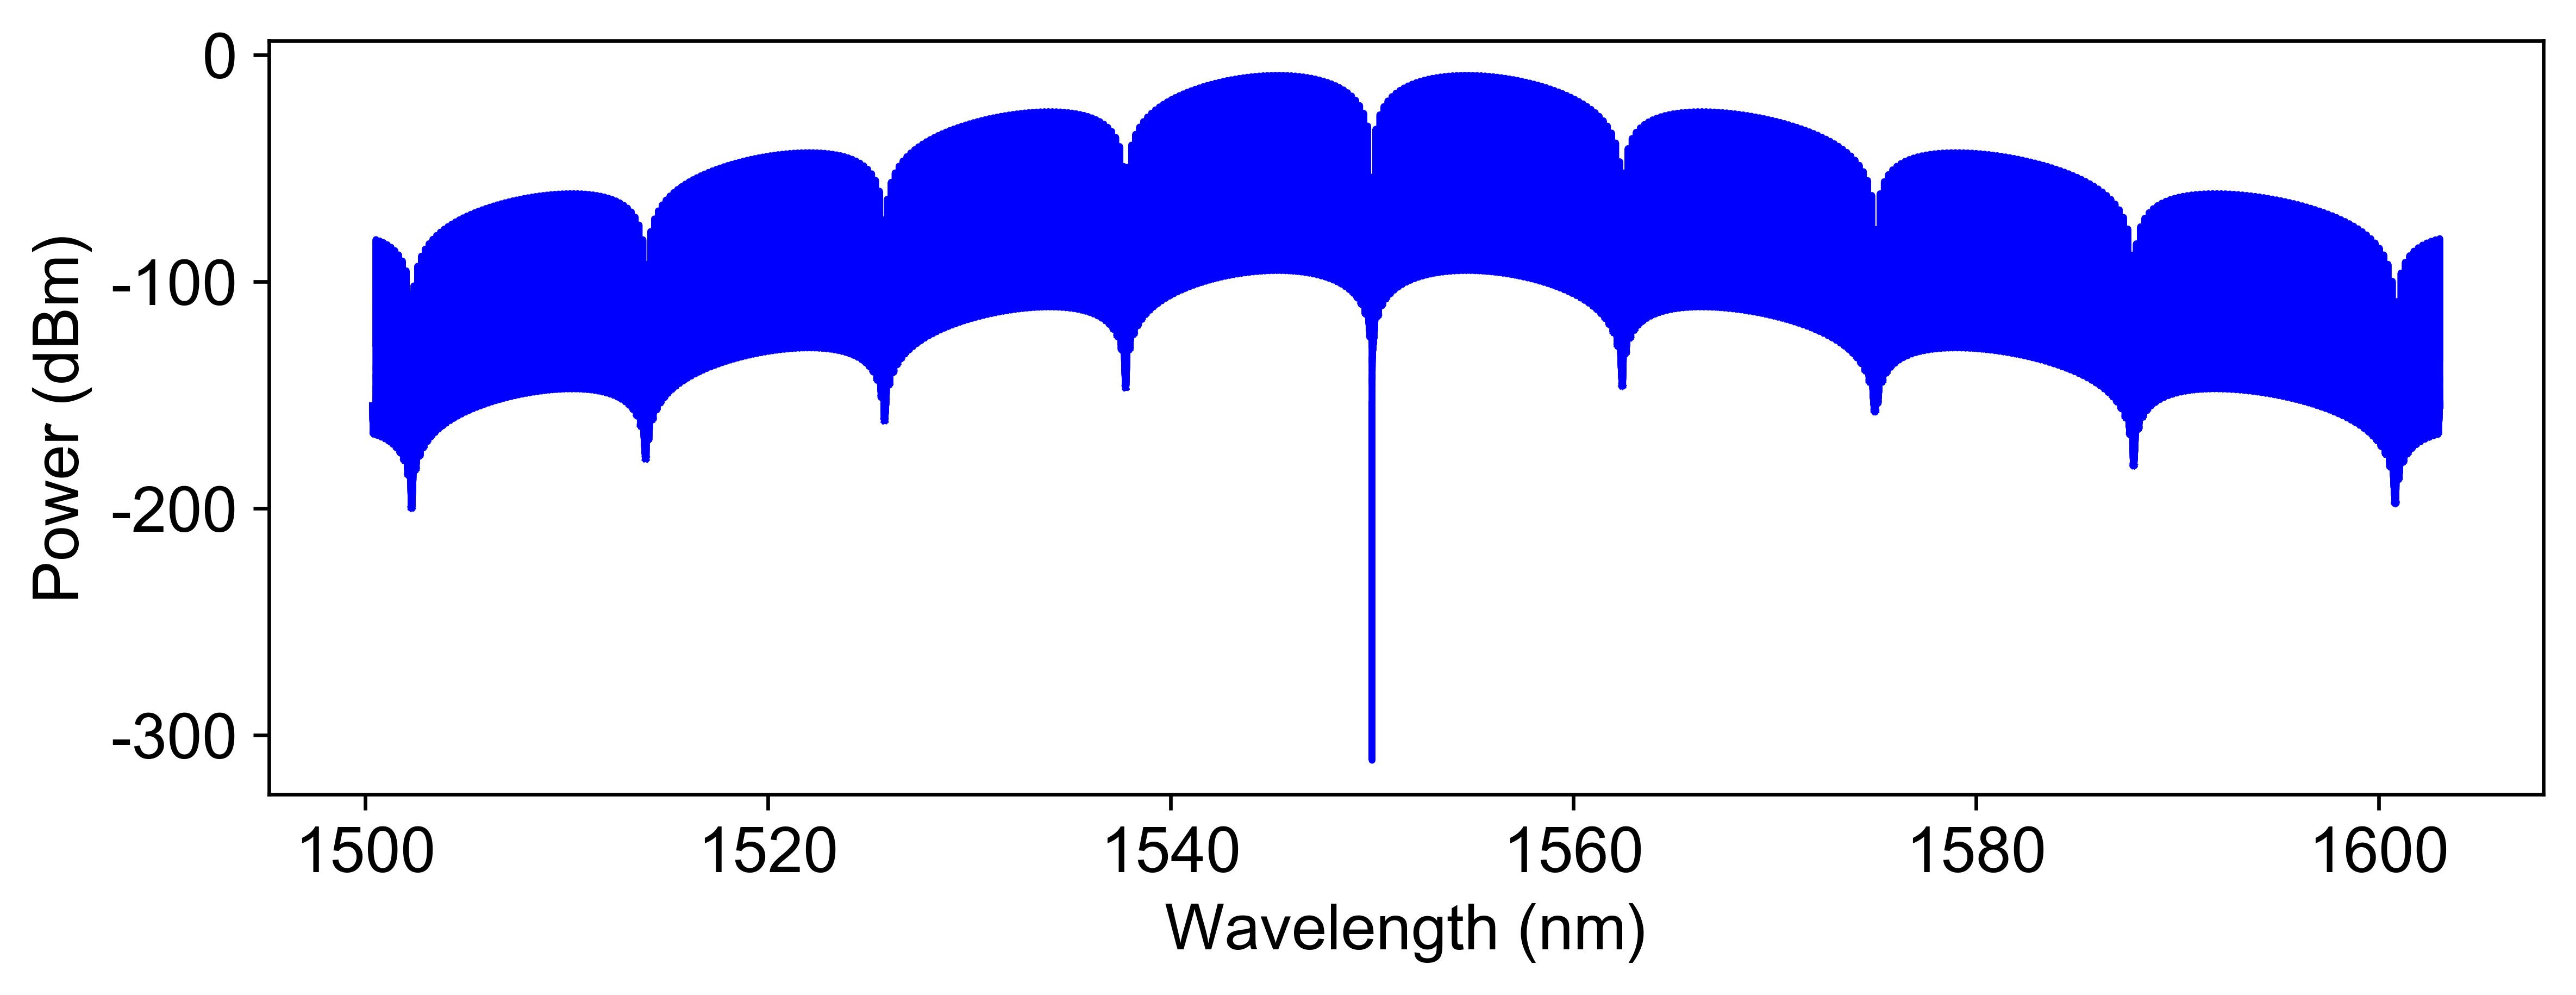
\includegraphics[width=0.48\linewidth]{figure/fig_14_0.png}
    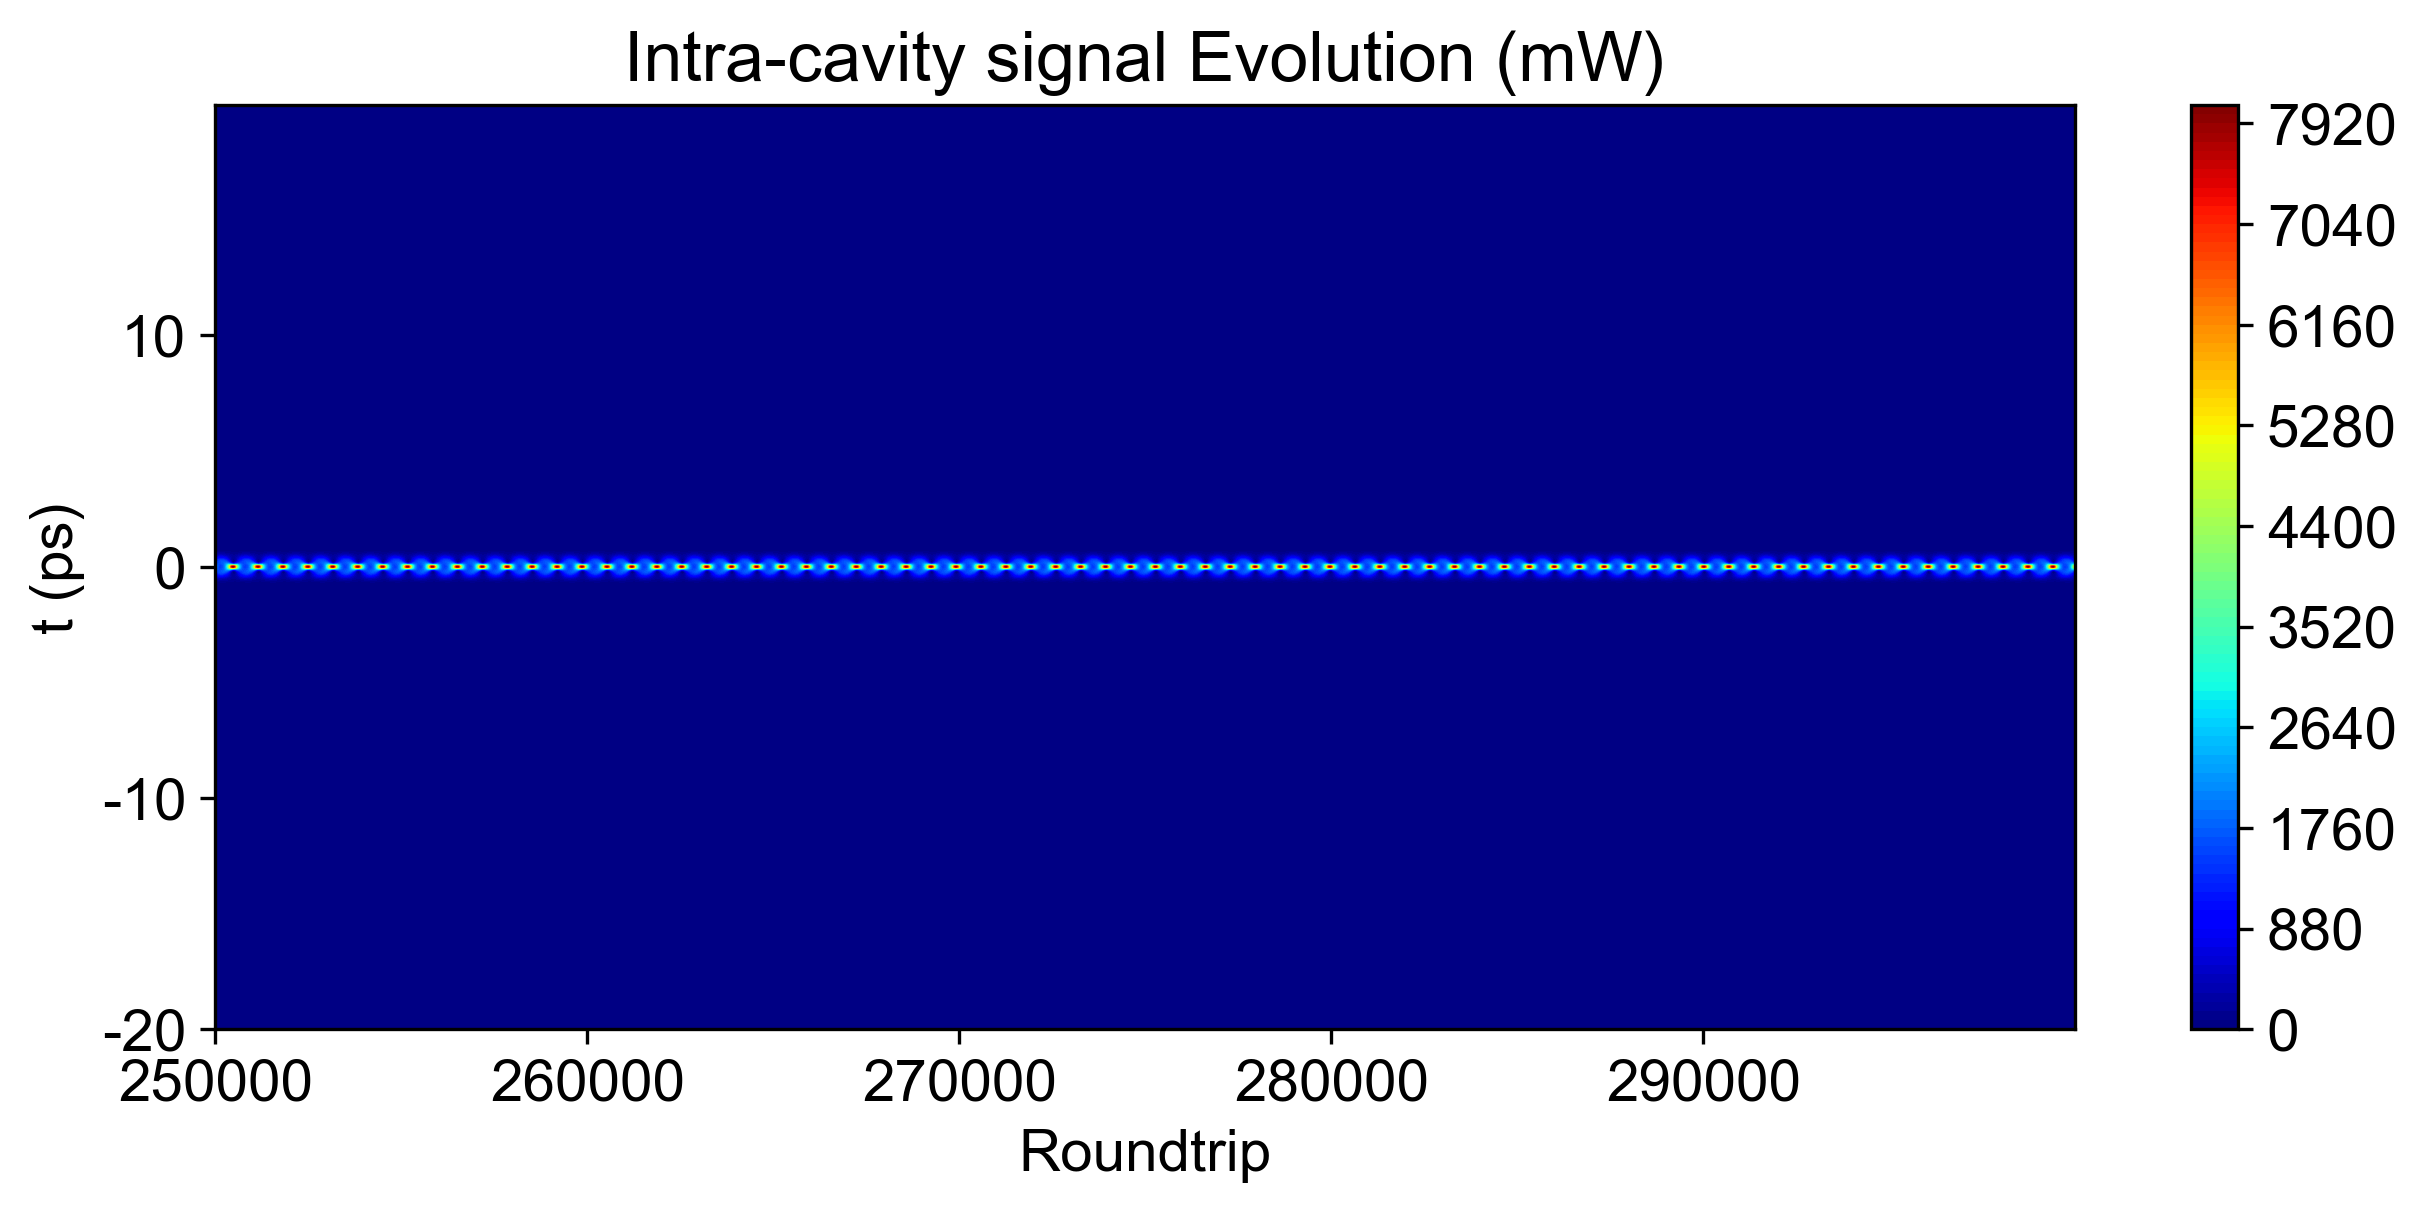
\includegraphics[width=0.48\linewidth]{figure/fig_15.png}
    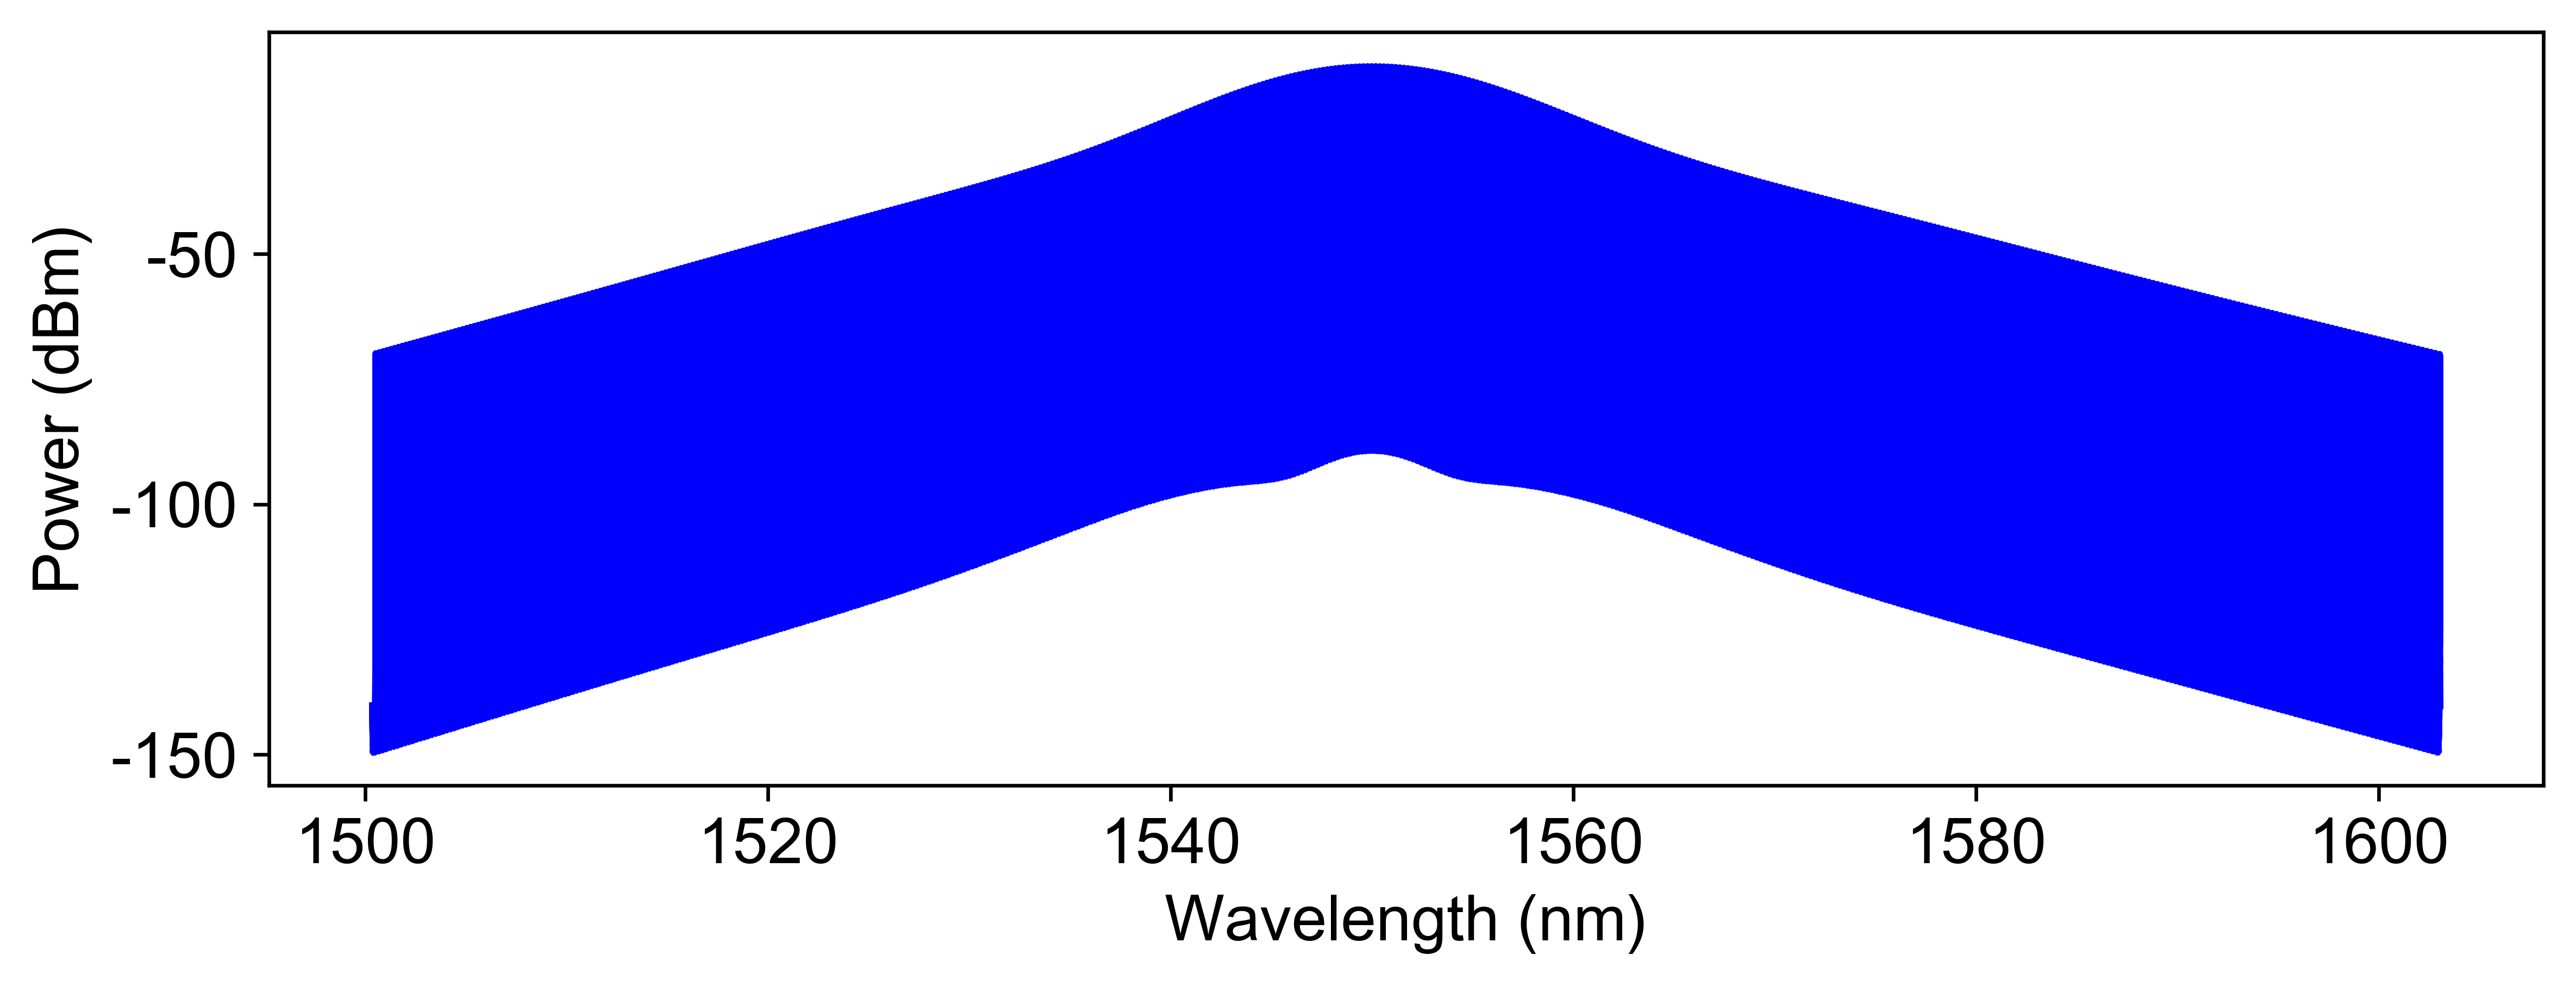
\includegraphics[width=0.48\linewidth]{figure/fig_15_0.png}
    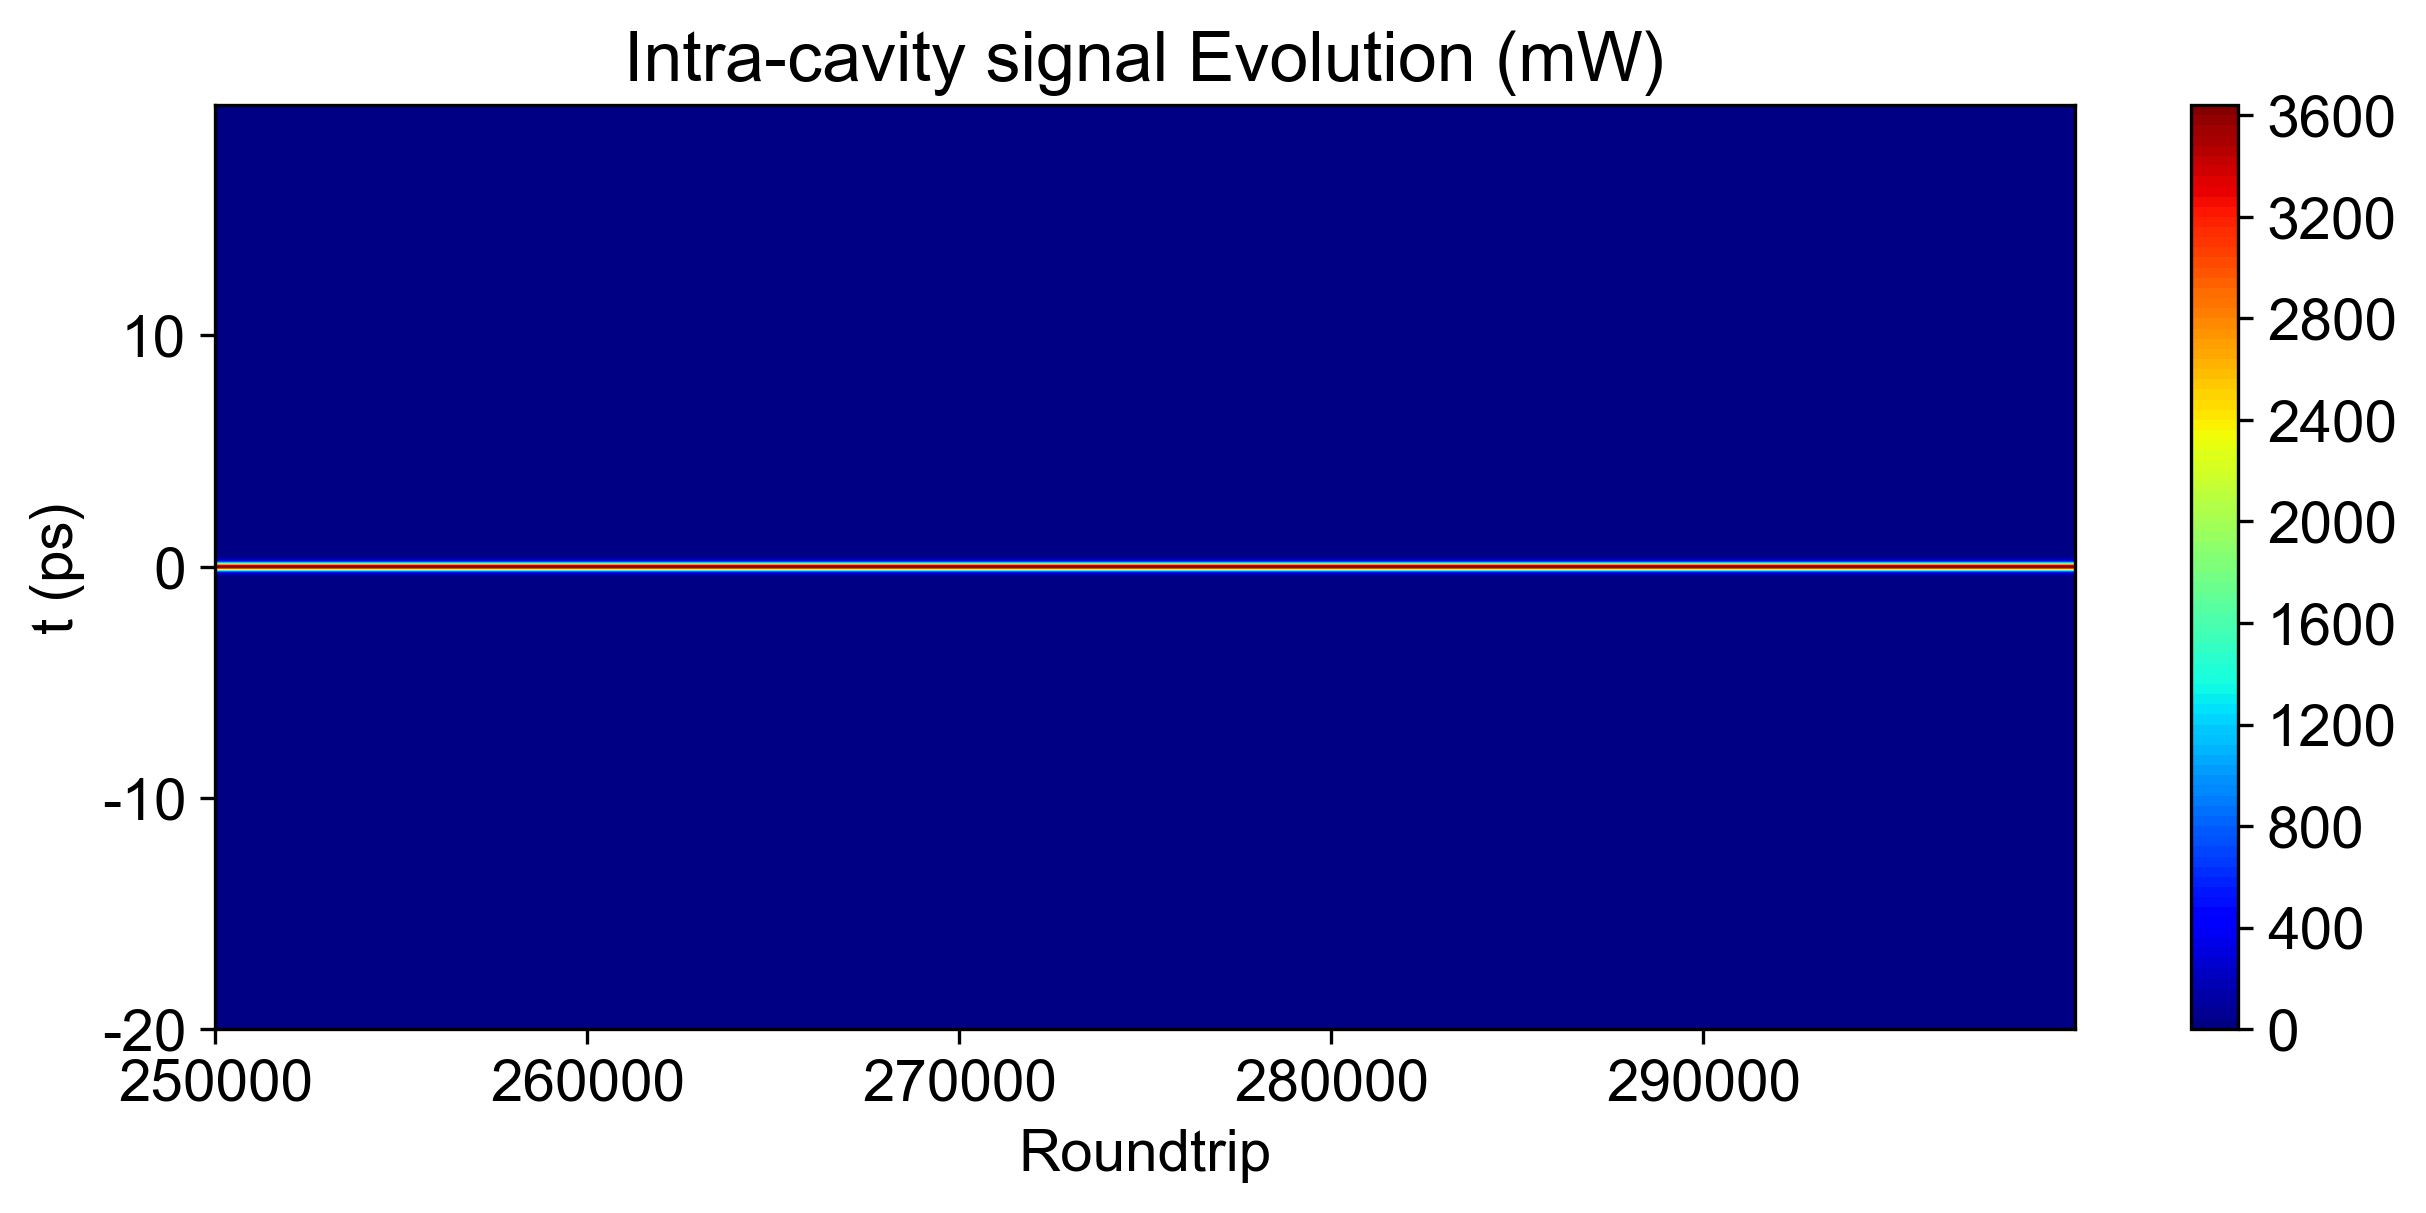
\includegraphics[width=0.48\linewidth]{figure/fig_16.png}
    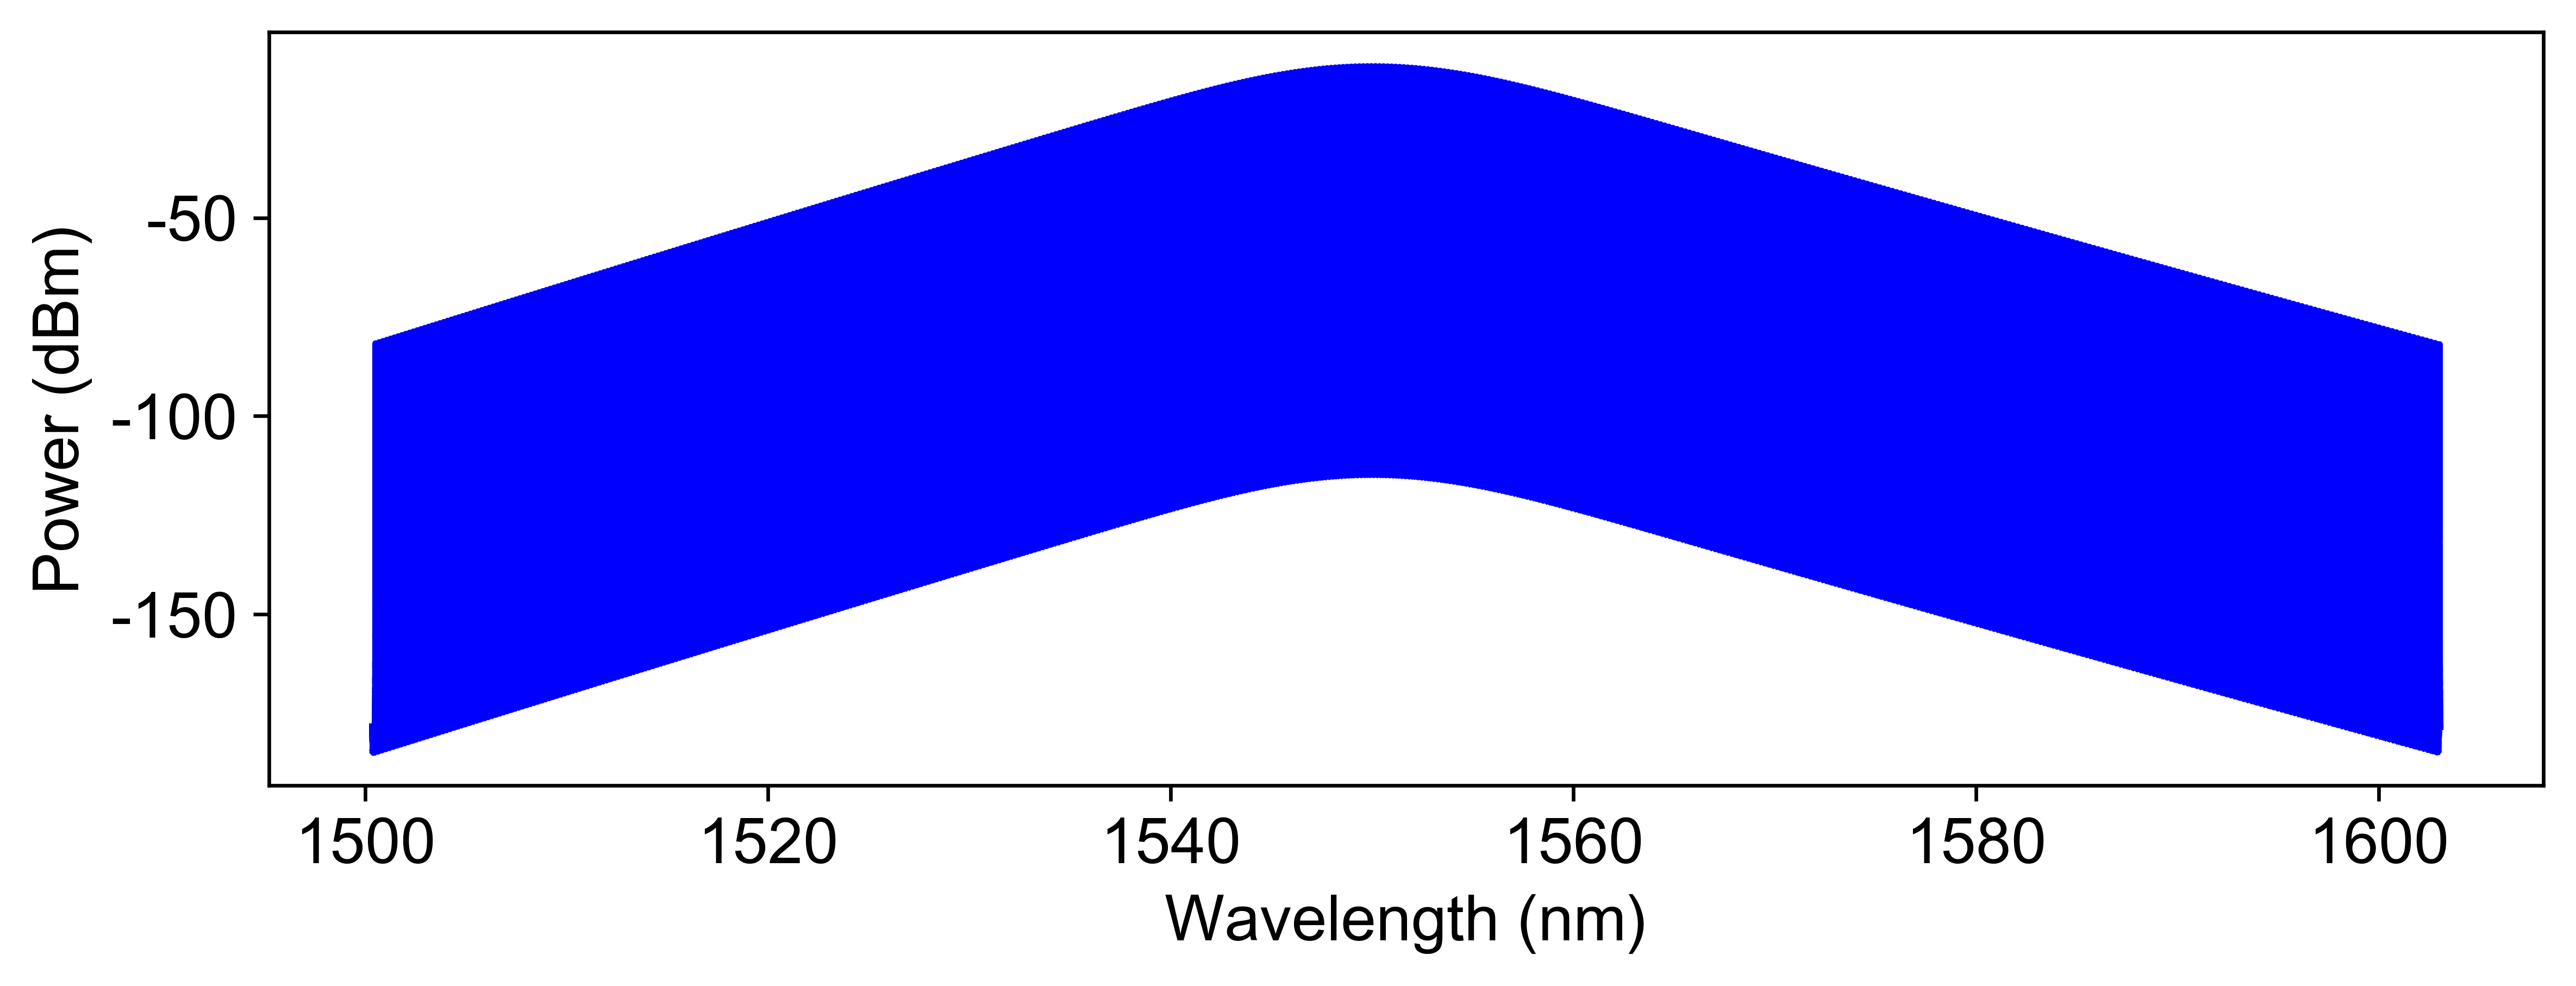
\includegraphics[width=0.48\linewidth]{figure/fig_16_0.png}
    \caption{左列:腔内信号光场的稳态,对应的光谱。从上到下调制深度依次为:0.1,0.3,0.5,0.7,1.0。}
    \label{fig:enter-label}
\end{figure}
调制深度越大,越接近锁模态。
\subsection{泵浦光功率}
以$FSR = 25GHz$,调制深度$M = 0.5$,改变泵浦功率进行仿真。\\
\begin{figure}[htbp]
    \centering
    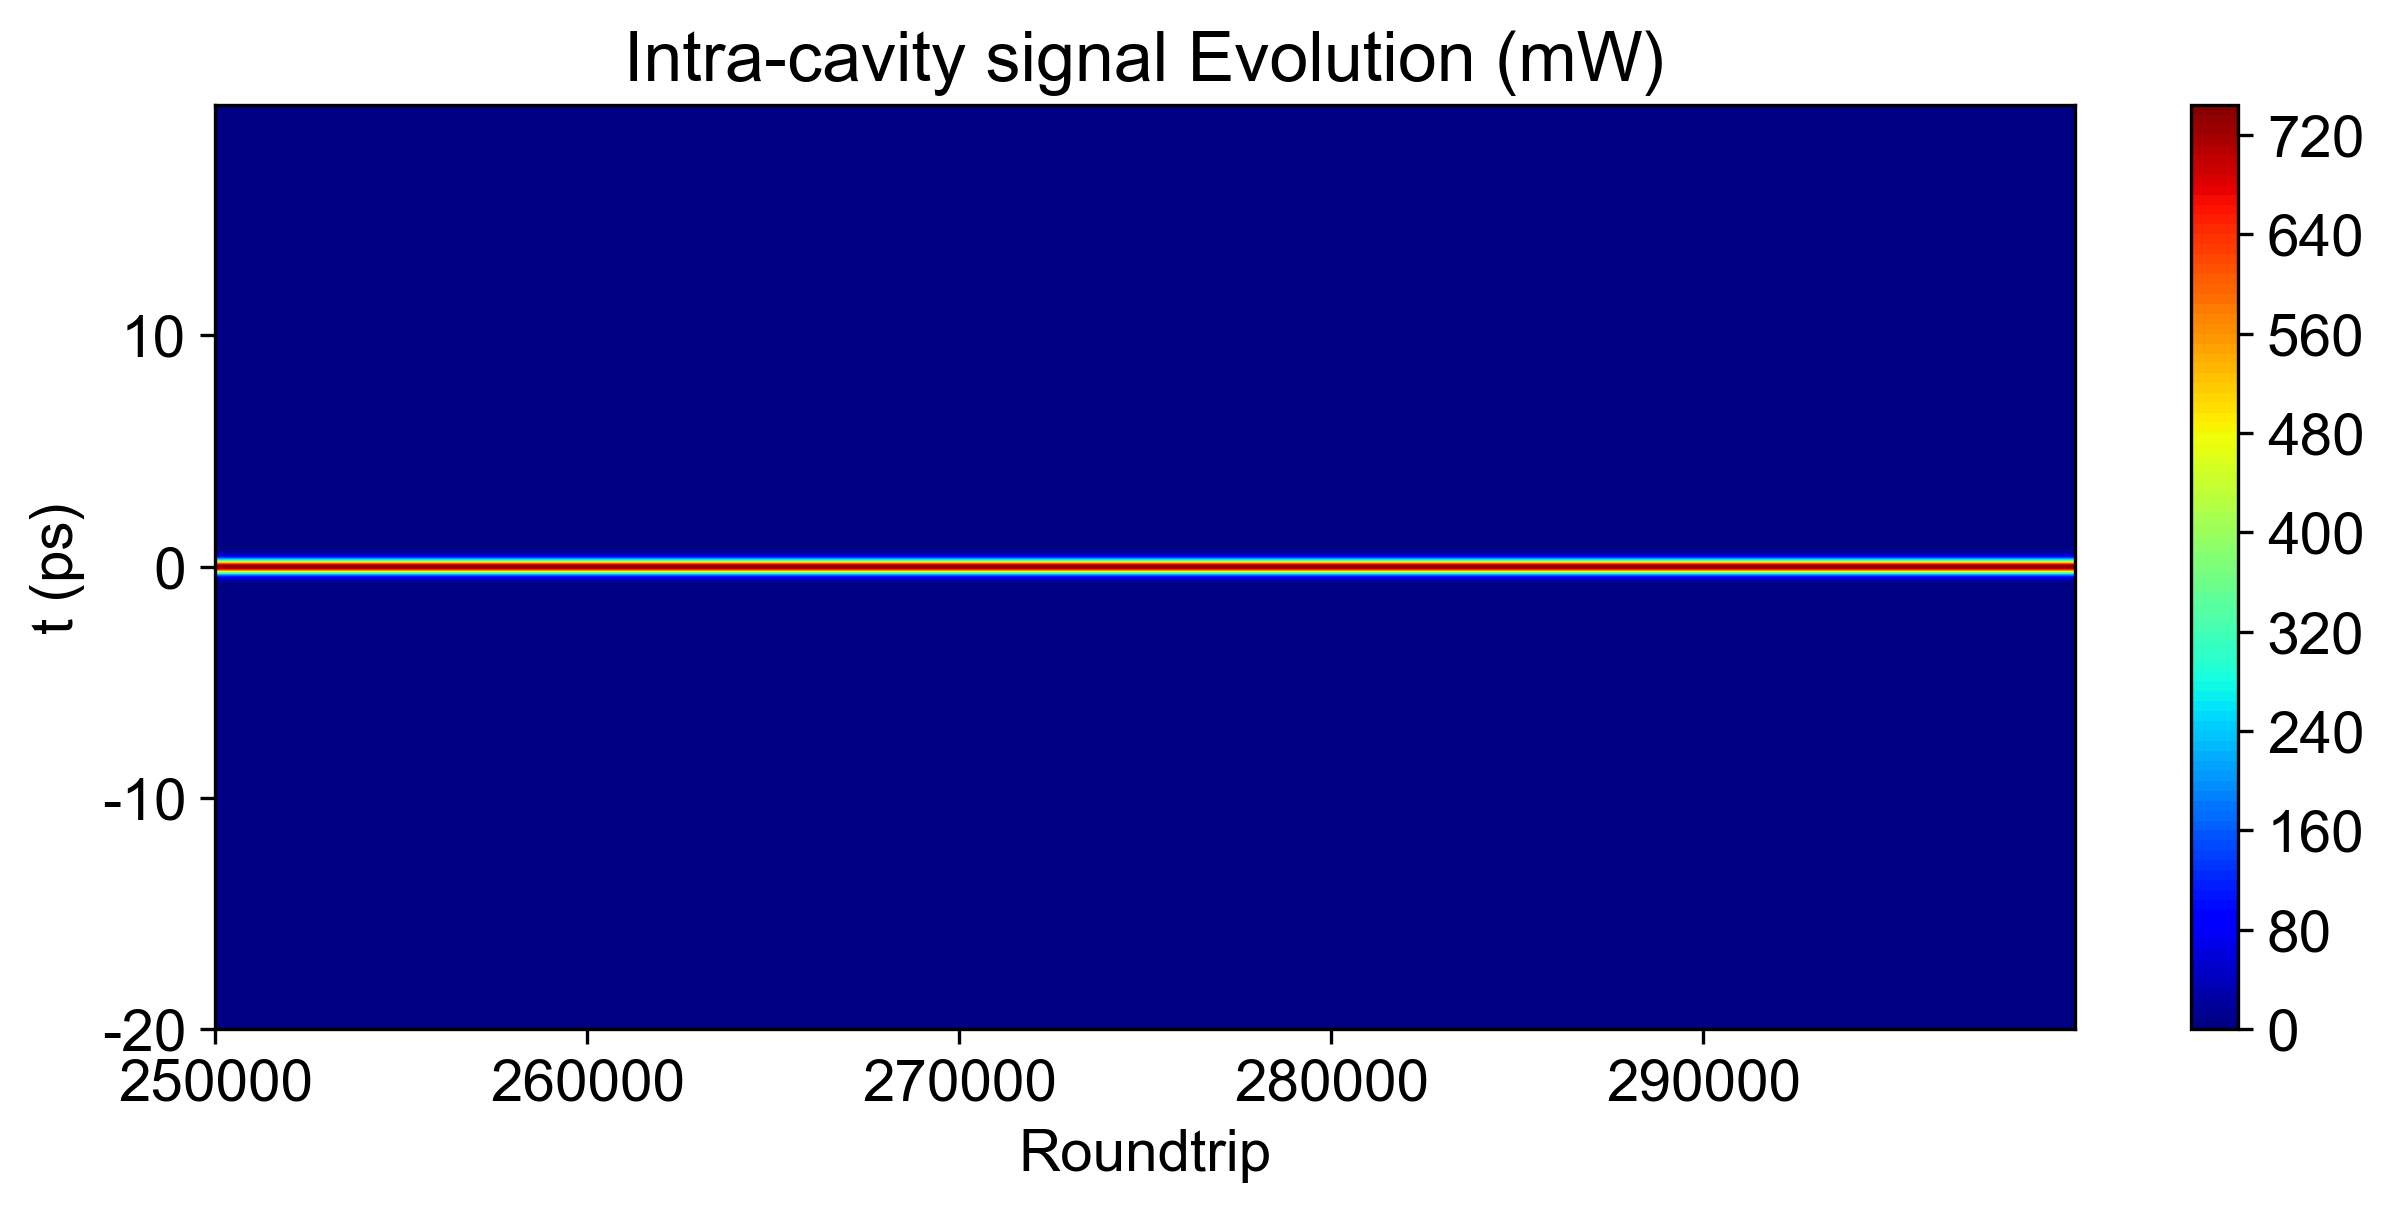
\includegraphics[width=0.48\linewidth]{figure/fig_17.png}
    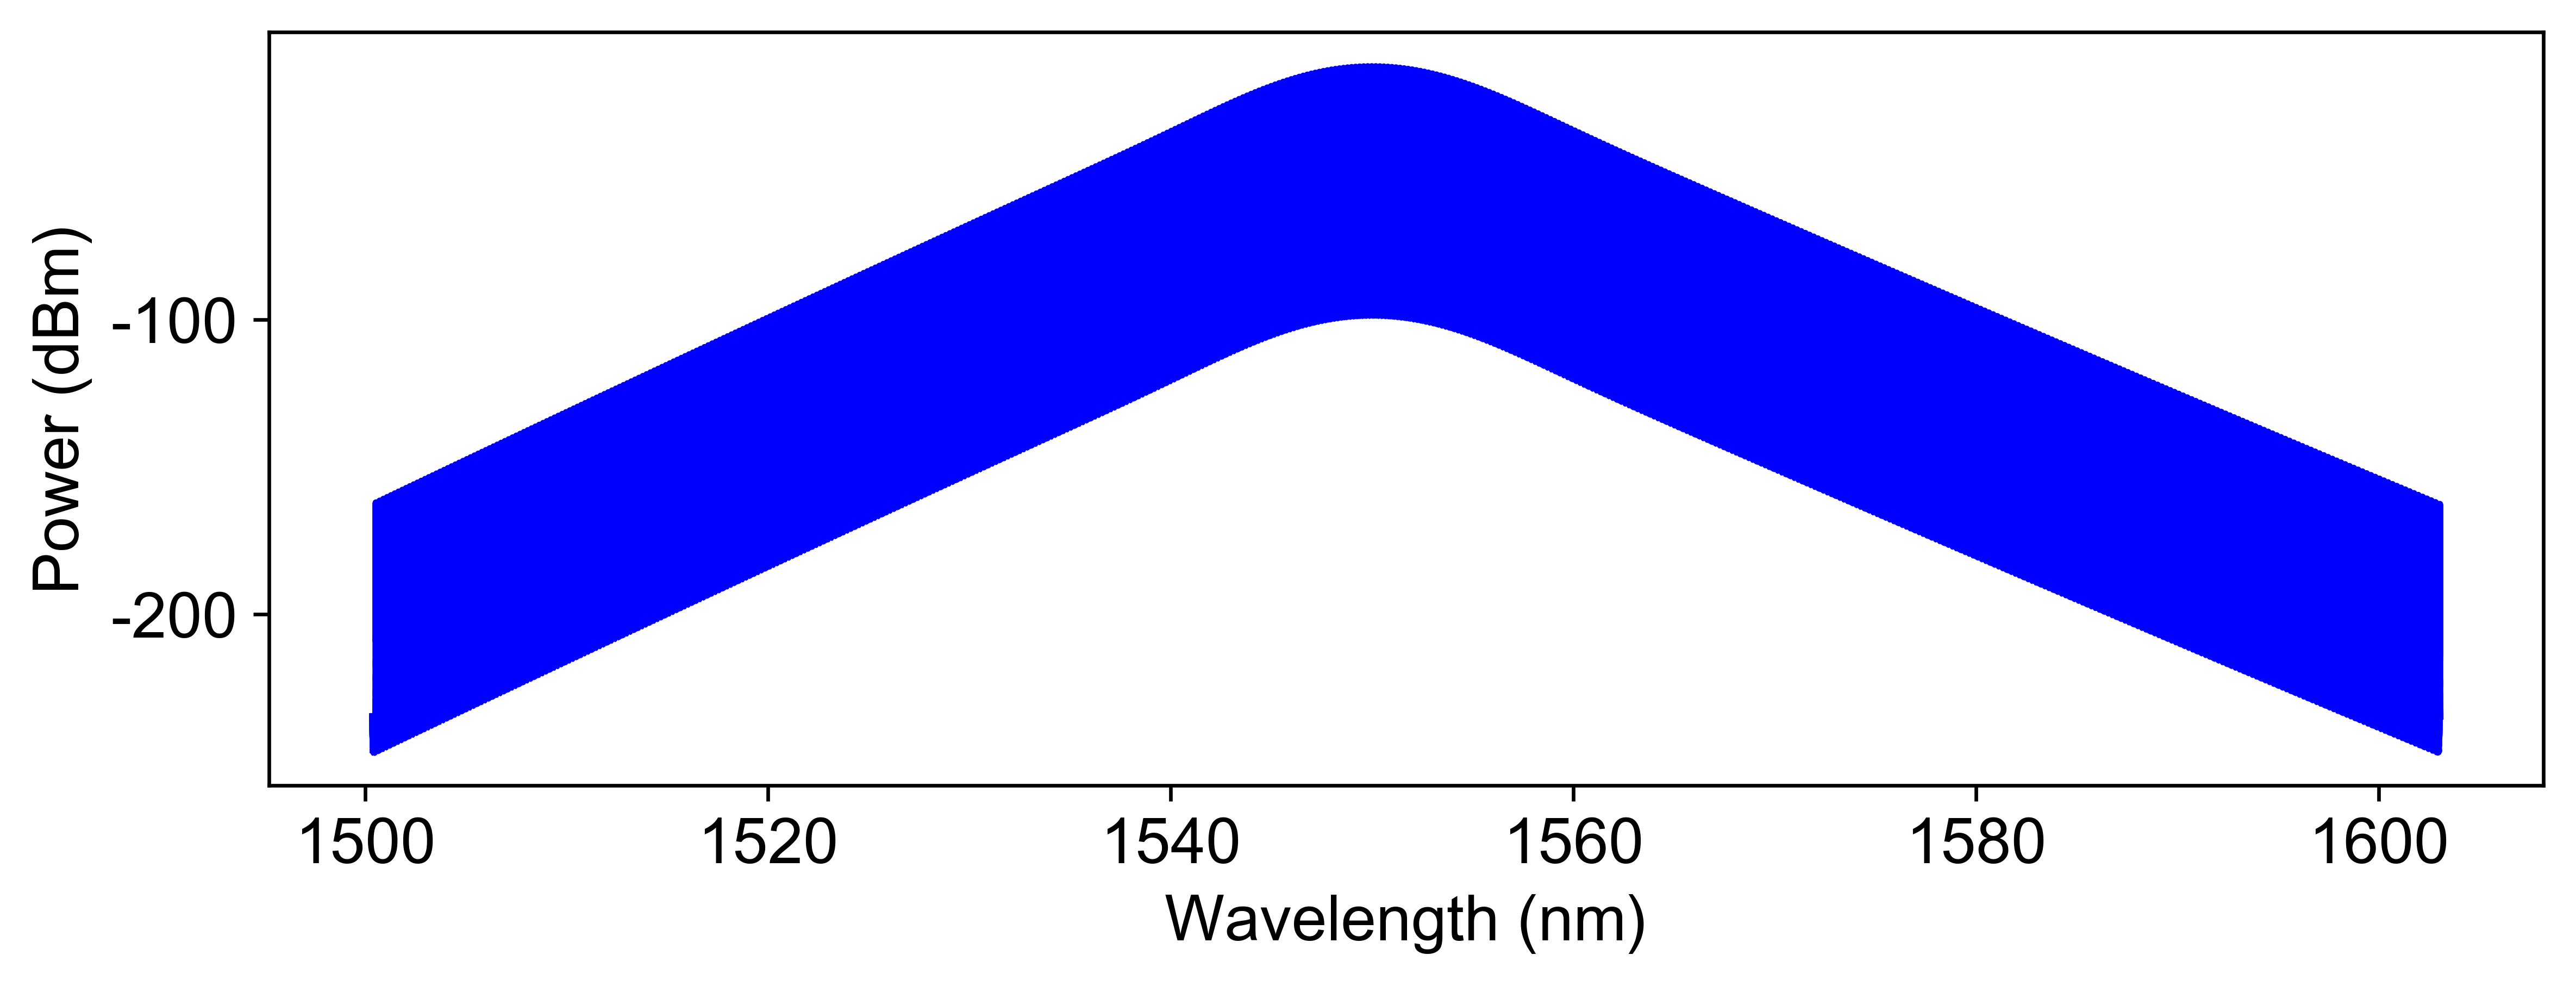
\includegraphics[width=0.48\linewidth]{figure/fig_17_0.png}
    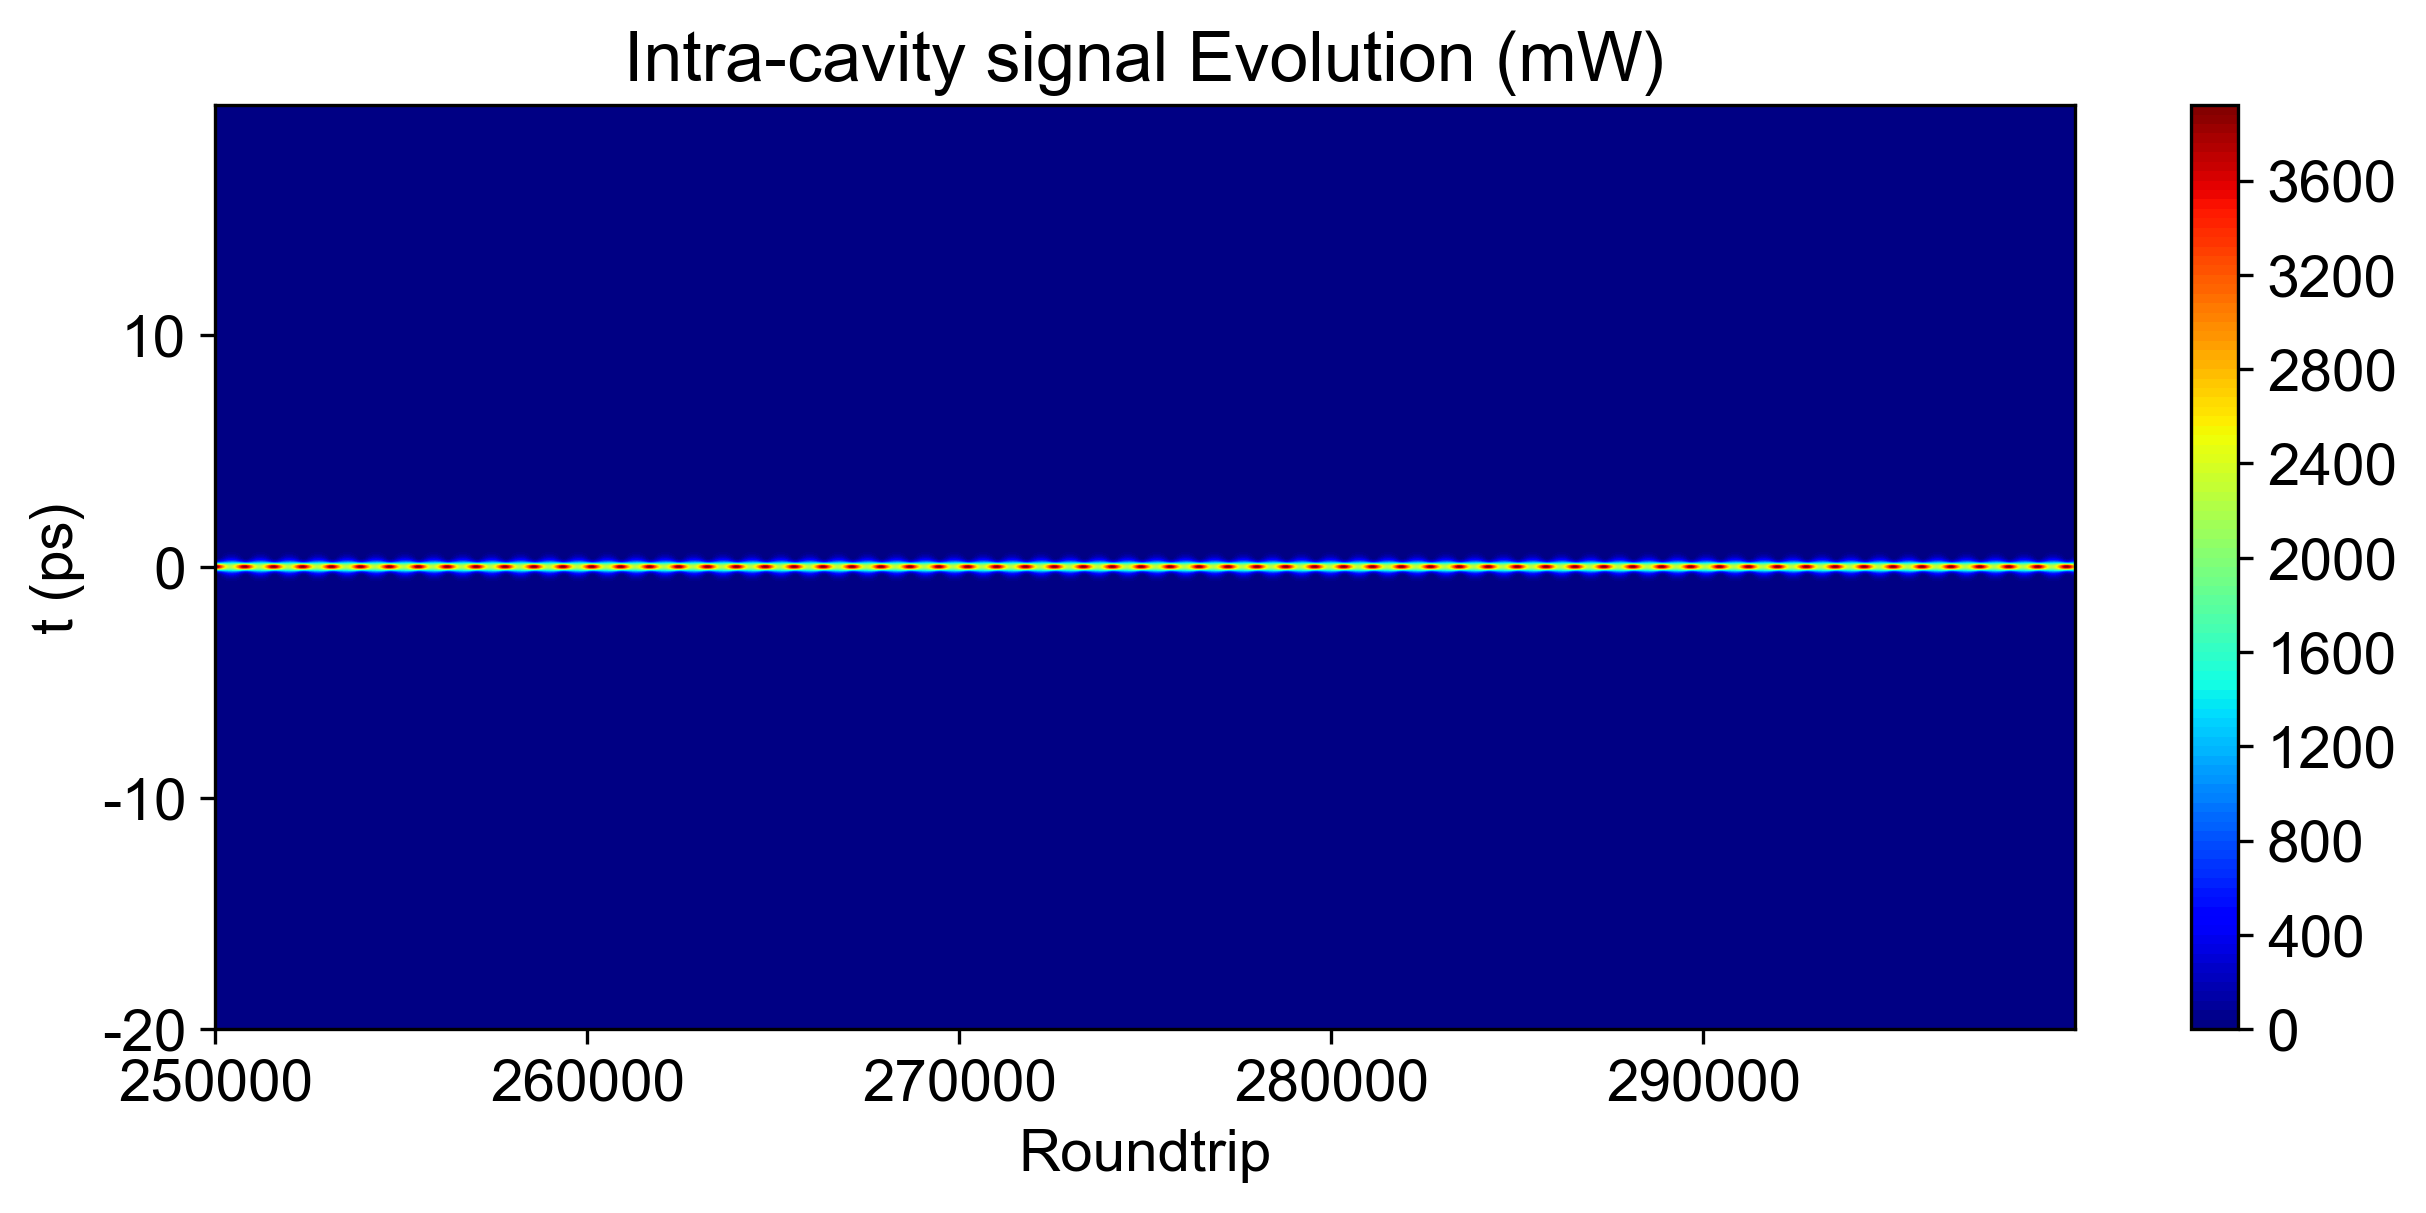
\includegraphics[width=0.48\linewidth]{figure/fig_18.png}
    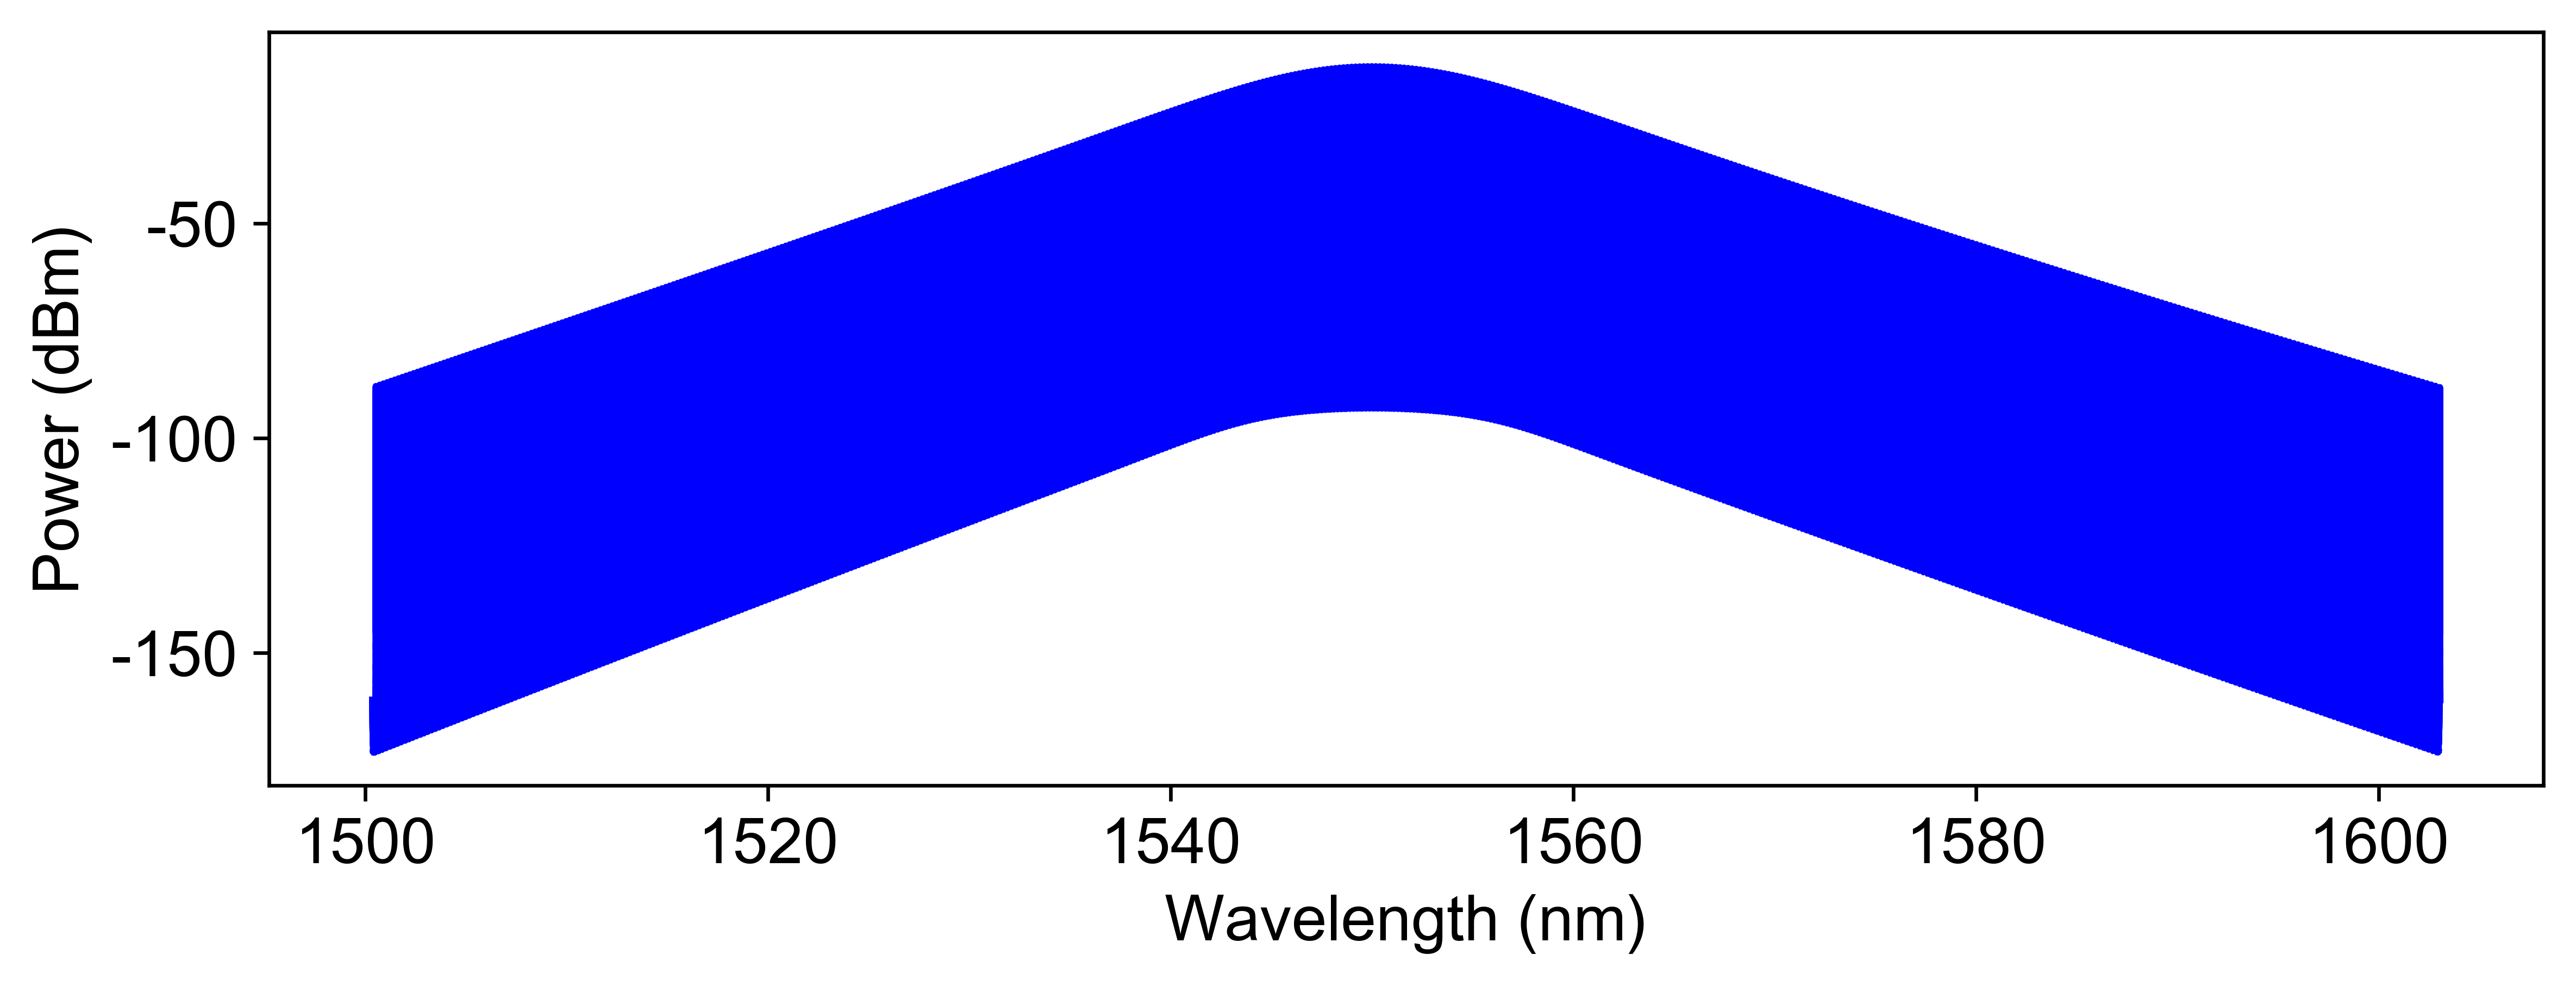
\includegraphics[width=0.48\linewidth]{figure/fig_18_0.png}
    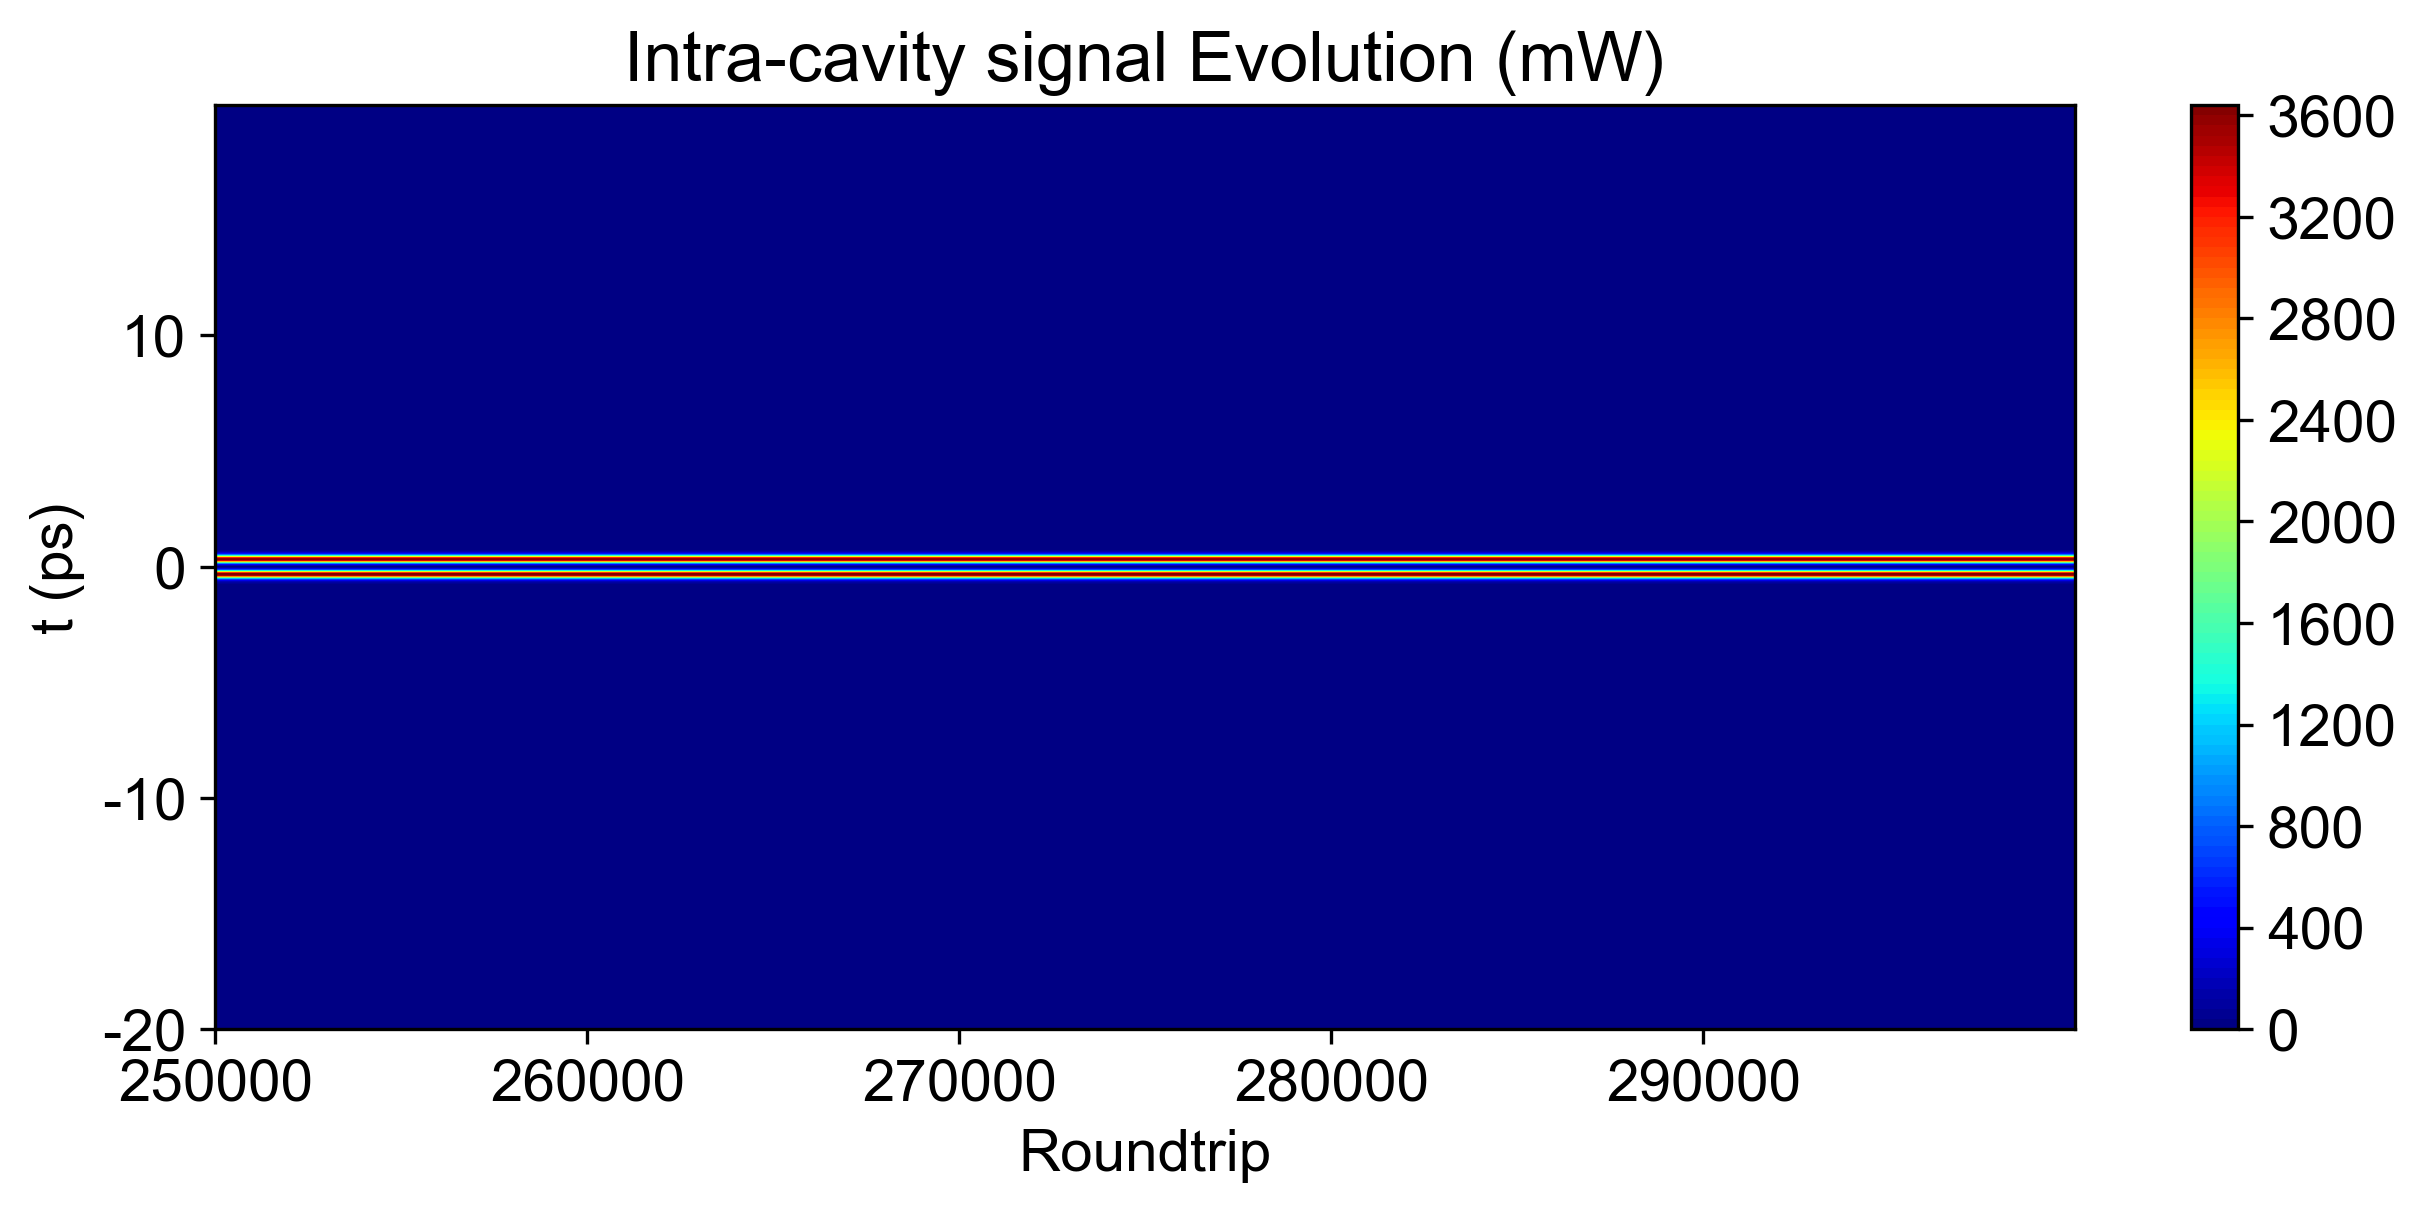
\includegraphics[width=0.48\linewidth]{figure/fig_19.png}
    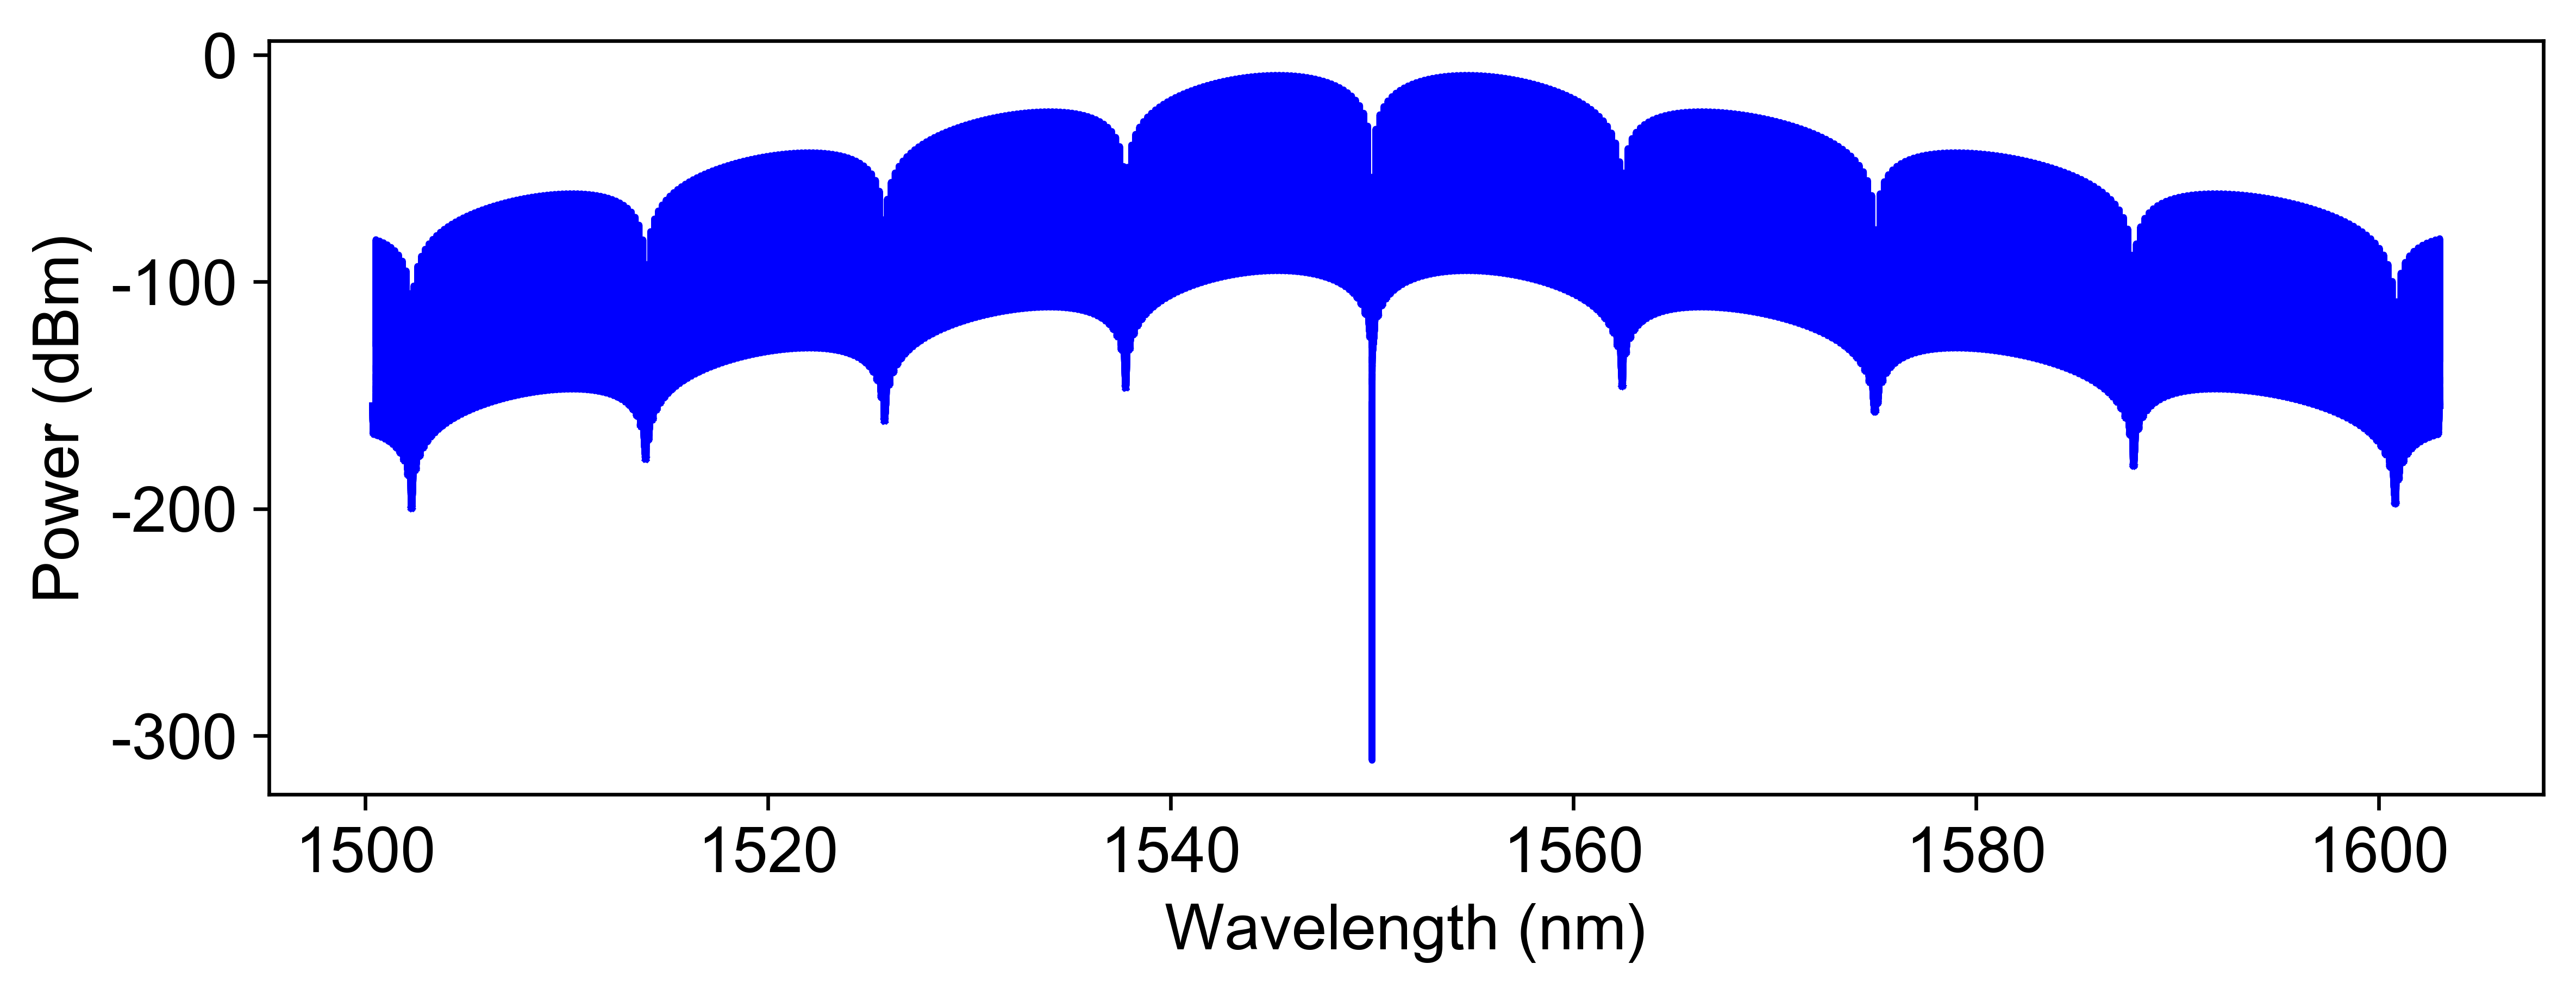
\includegraphics[width=0.48\linewidth]{figure/fig_19_0.png}
    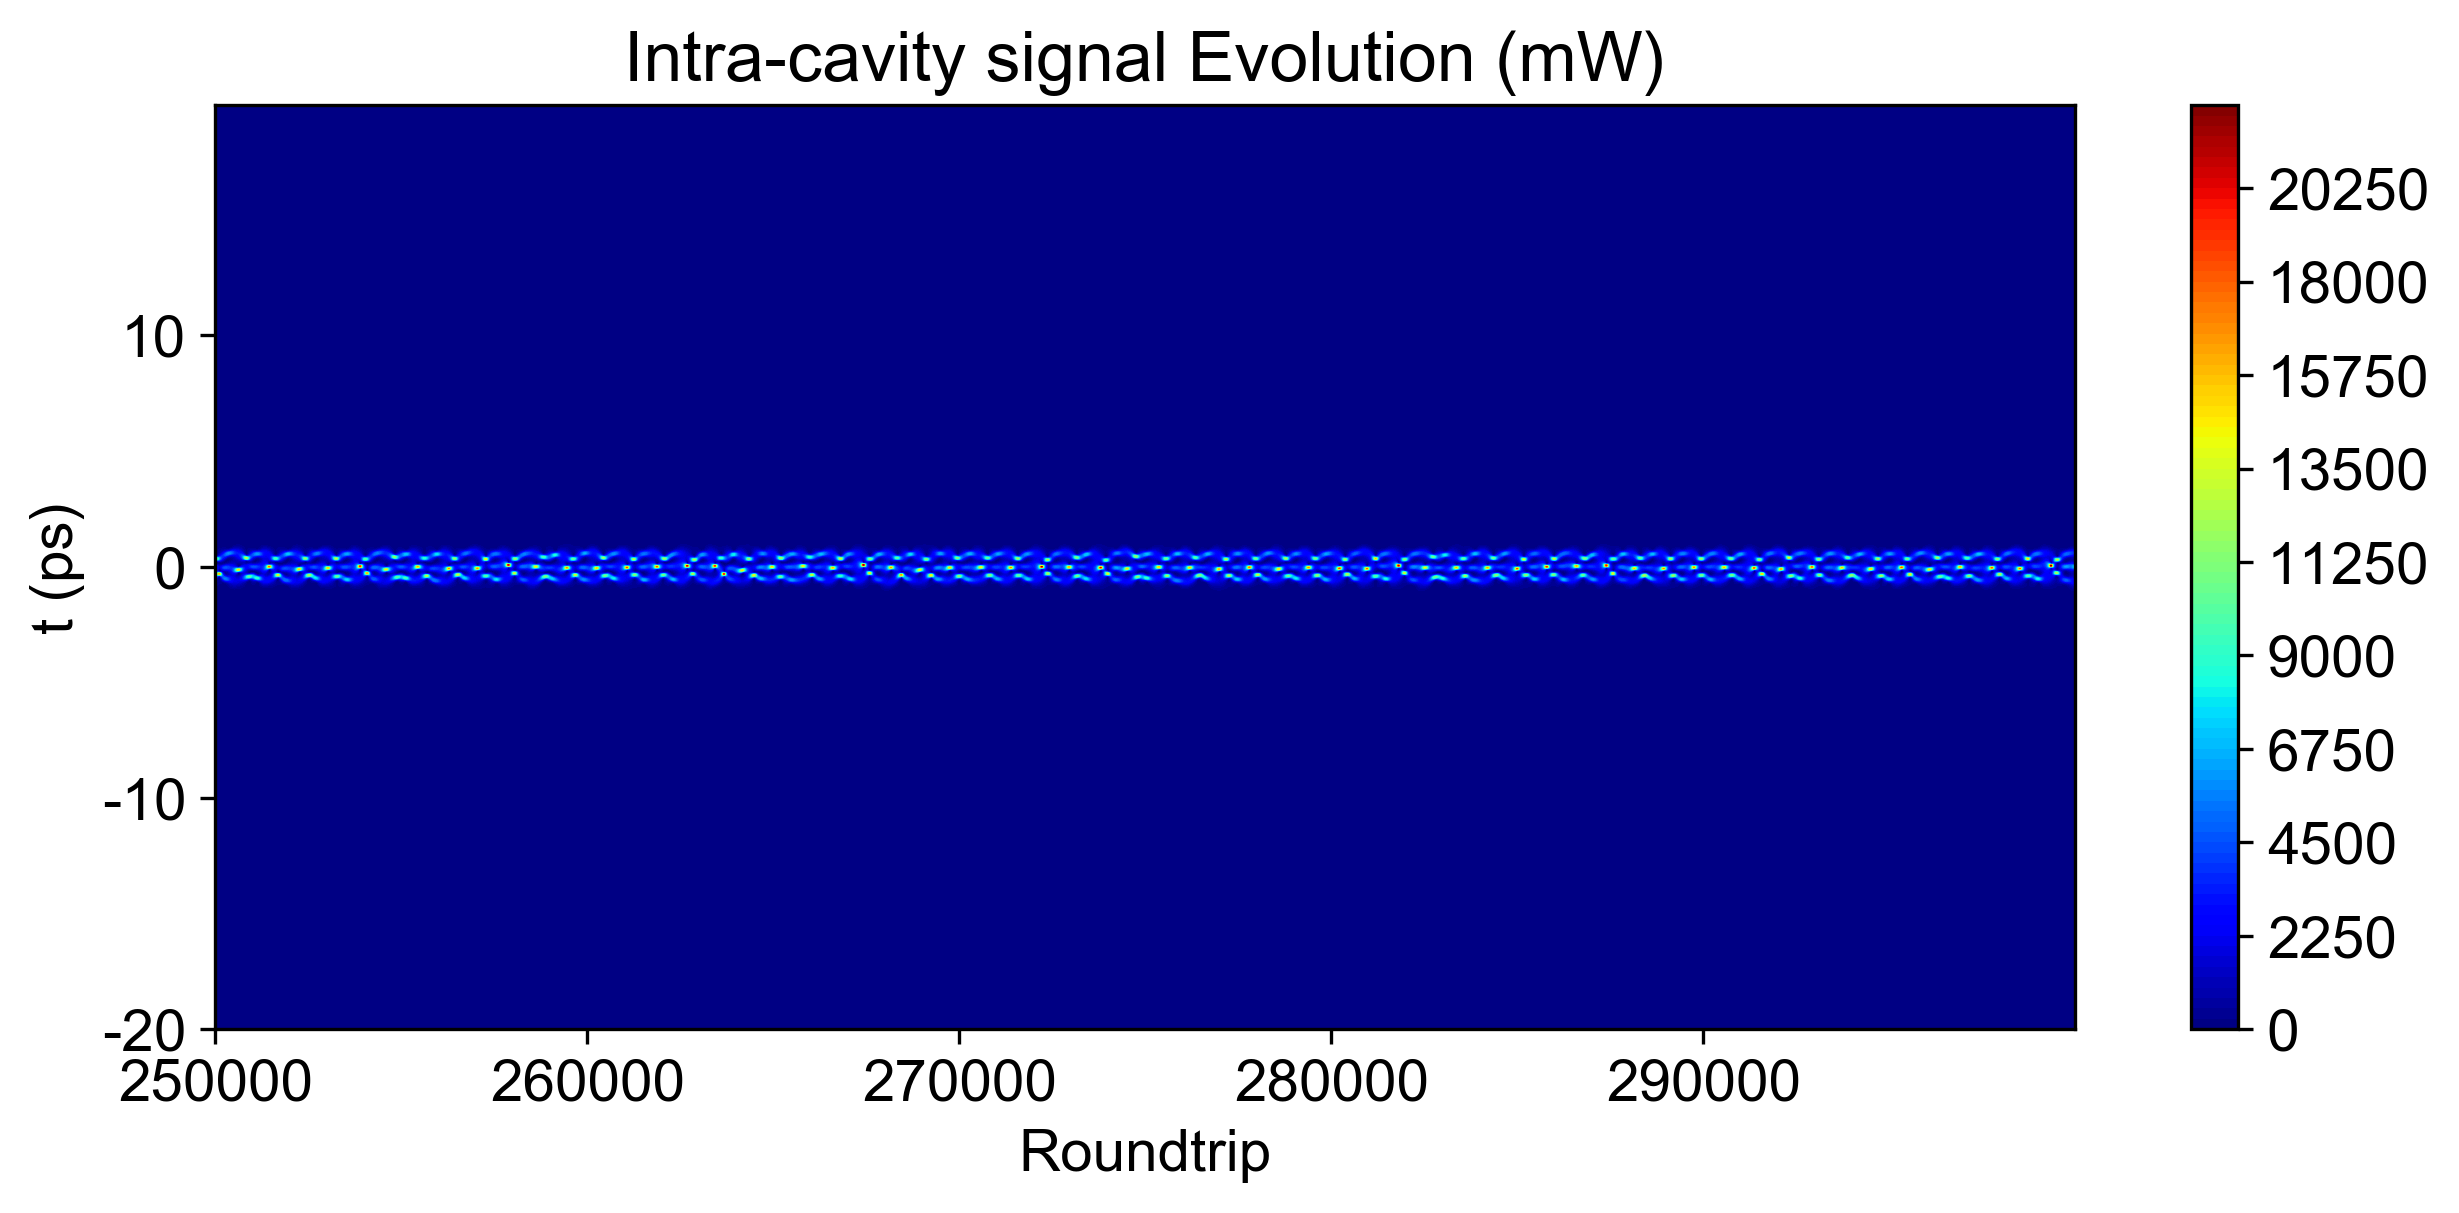
\includegraphics[width=0.48\linewidth]{figure/fig_20.png}
    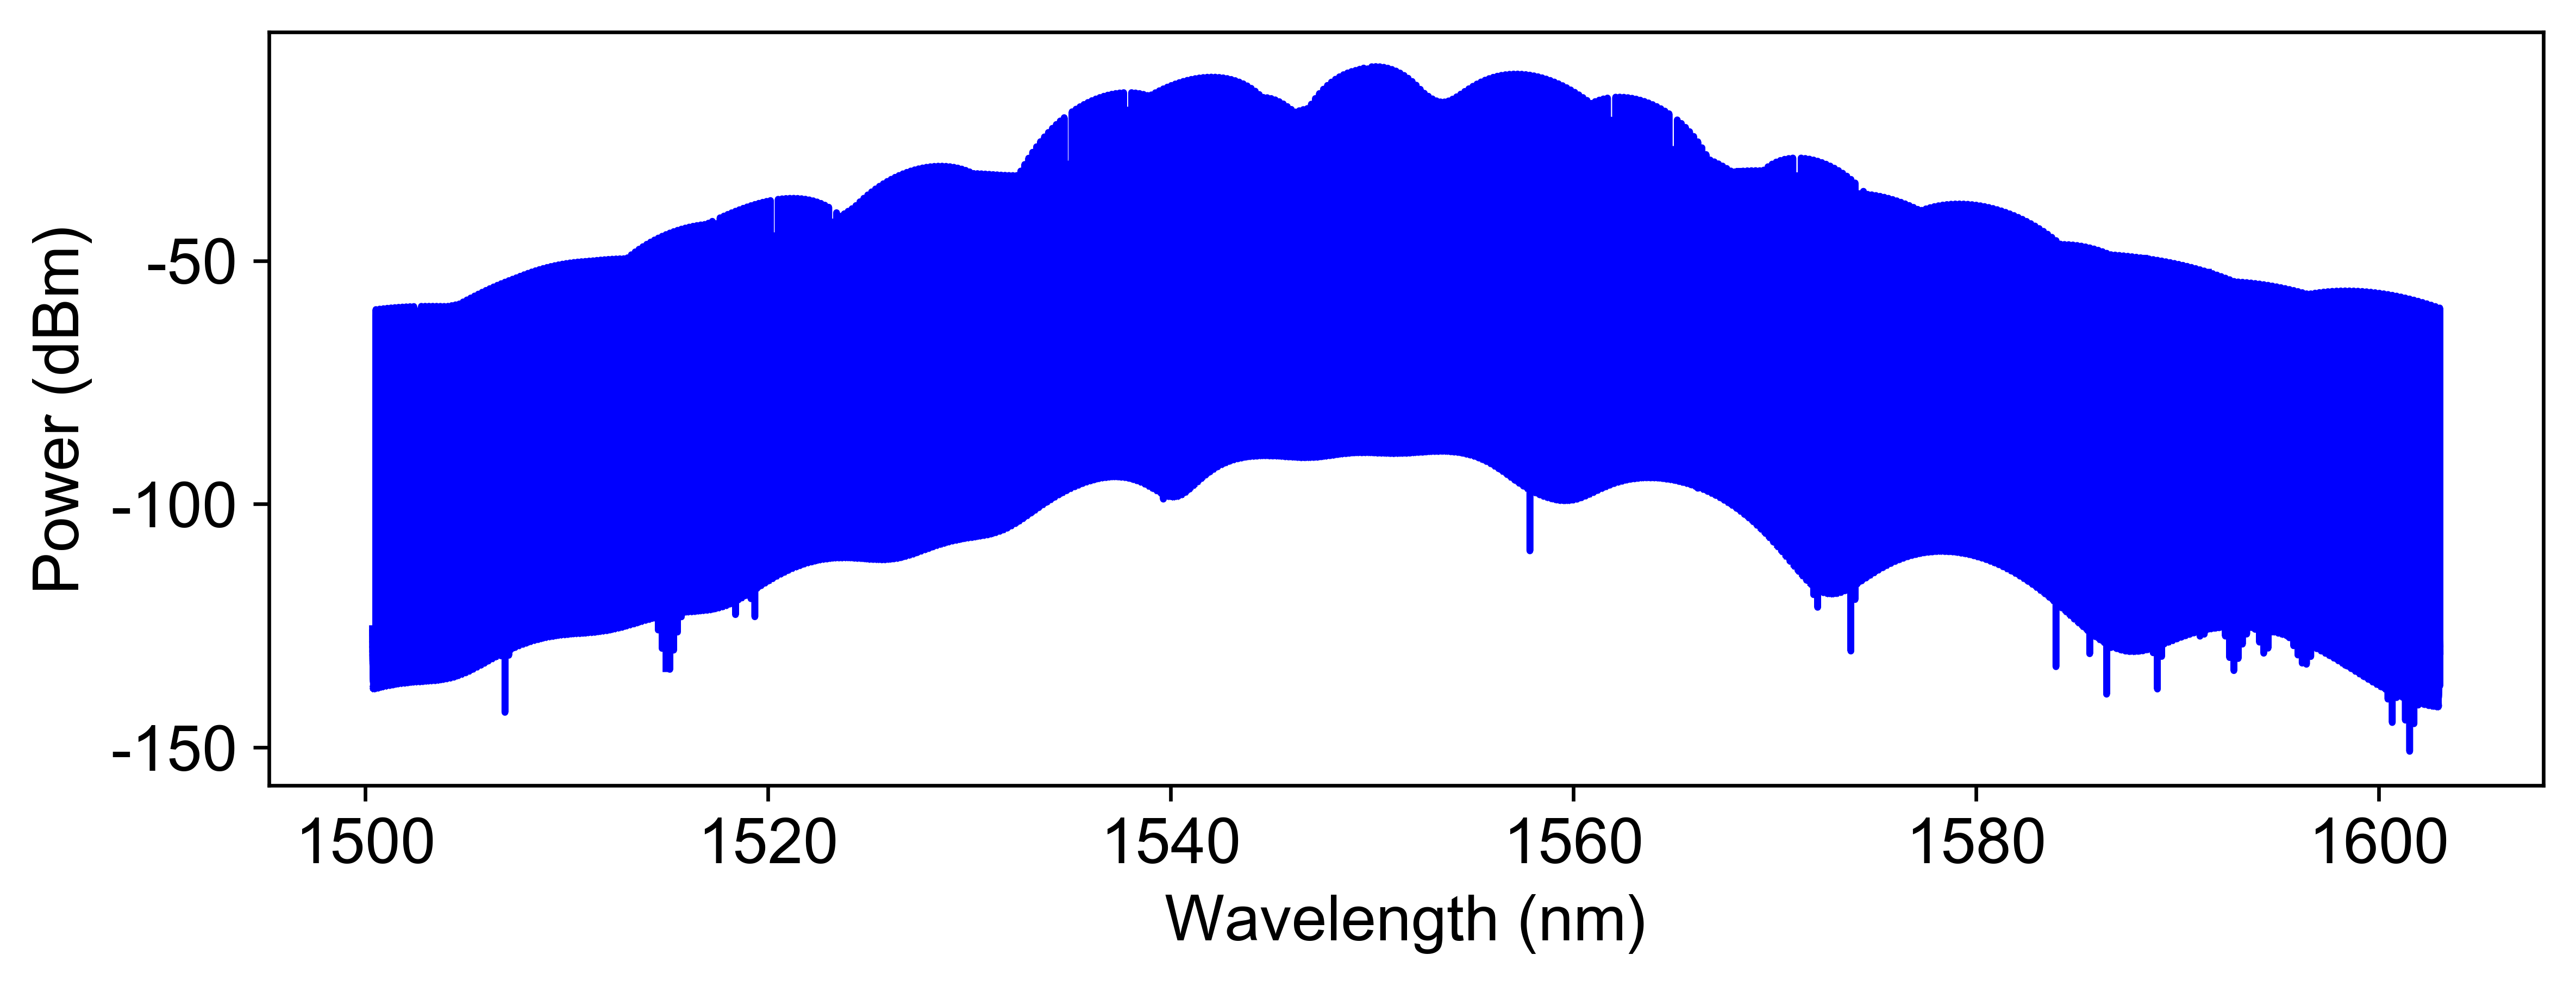
\includegraphics[width=0.48\linewidth]{figure/fig_20_0.png}
    \caption{左列:腔内信号光场的稳态,对应的光谱。从上到下泵浦功率依次为:20,50,100,200毫瓦。}
    \label{fig:enter-label}
\end{figure}
泵浦功率越小,越接近锁模态。
\subsection{重频}
以调制深度$M = 0.5$,泵浦功率$P_{in} = 100mW$,改变$FSR$进行仿真。\\
\begin{figure}[htbp]
    \centering
    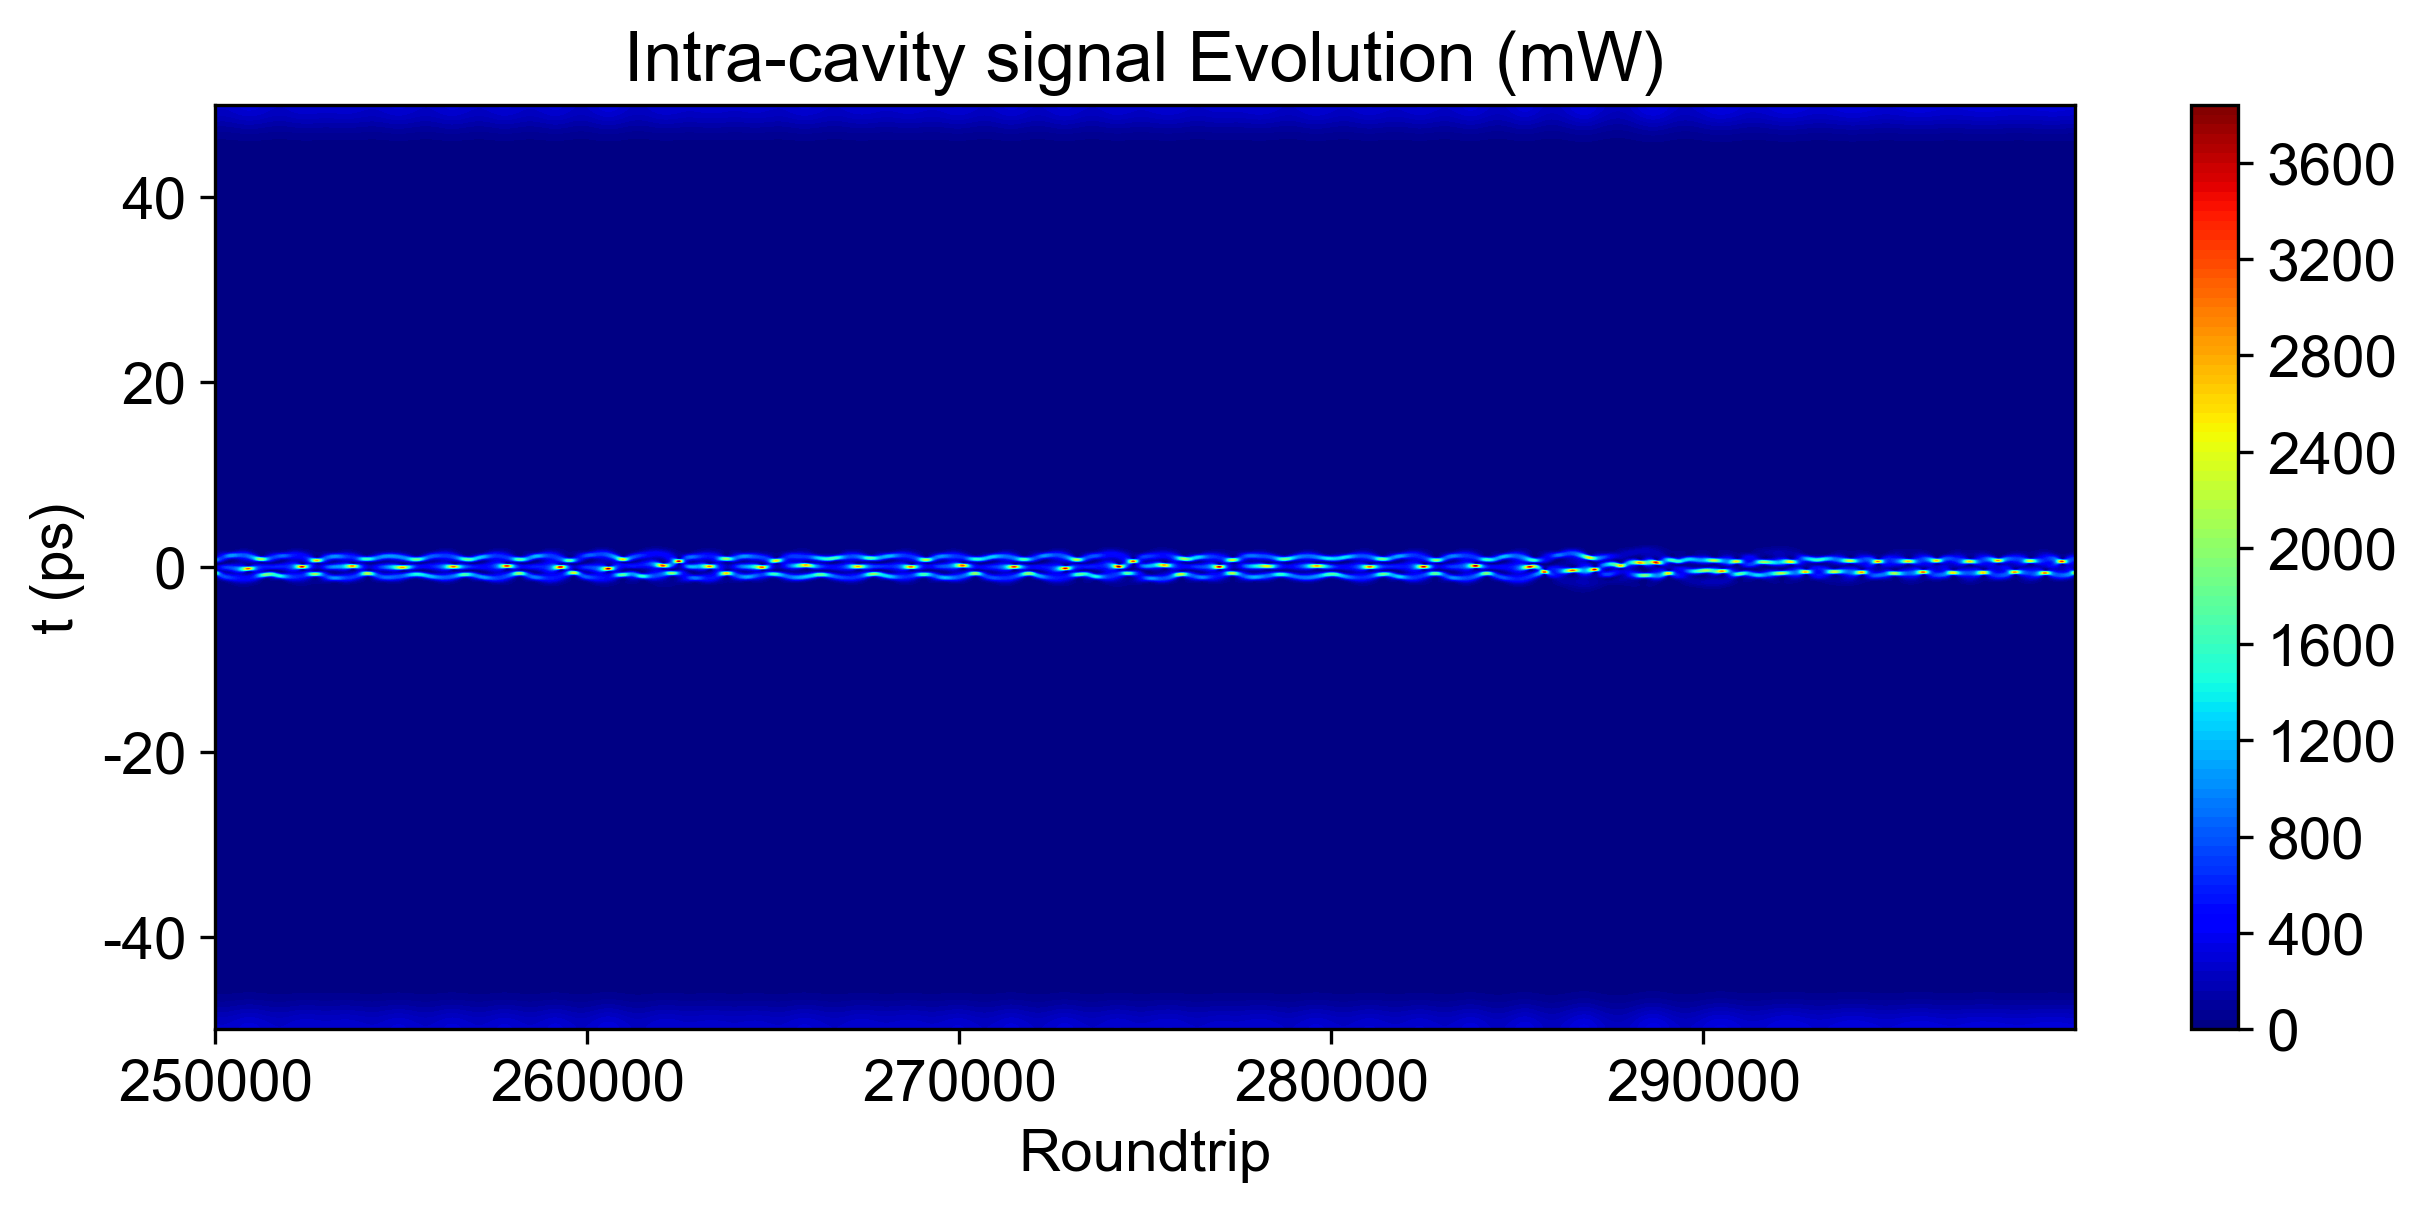
\includegraphics[width=0.48\linewidth]{figure/fig_21.png}
    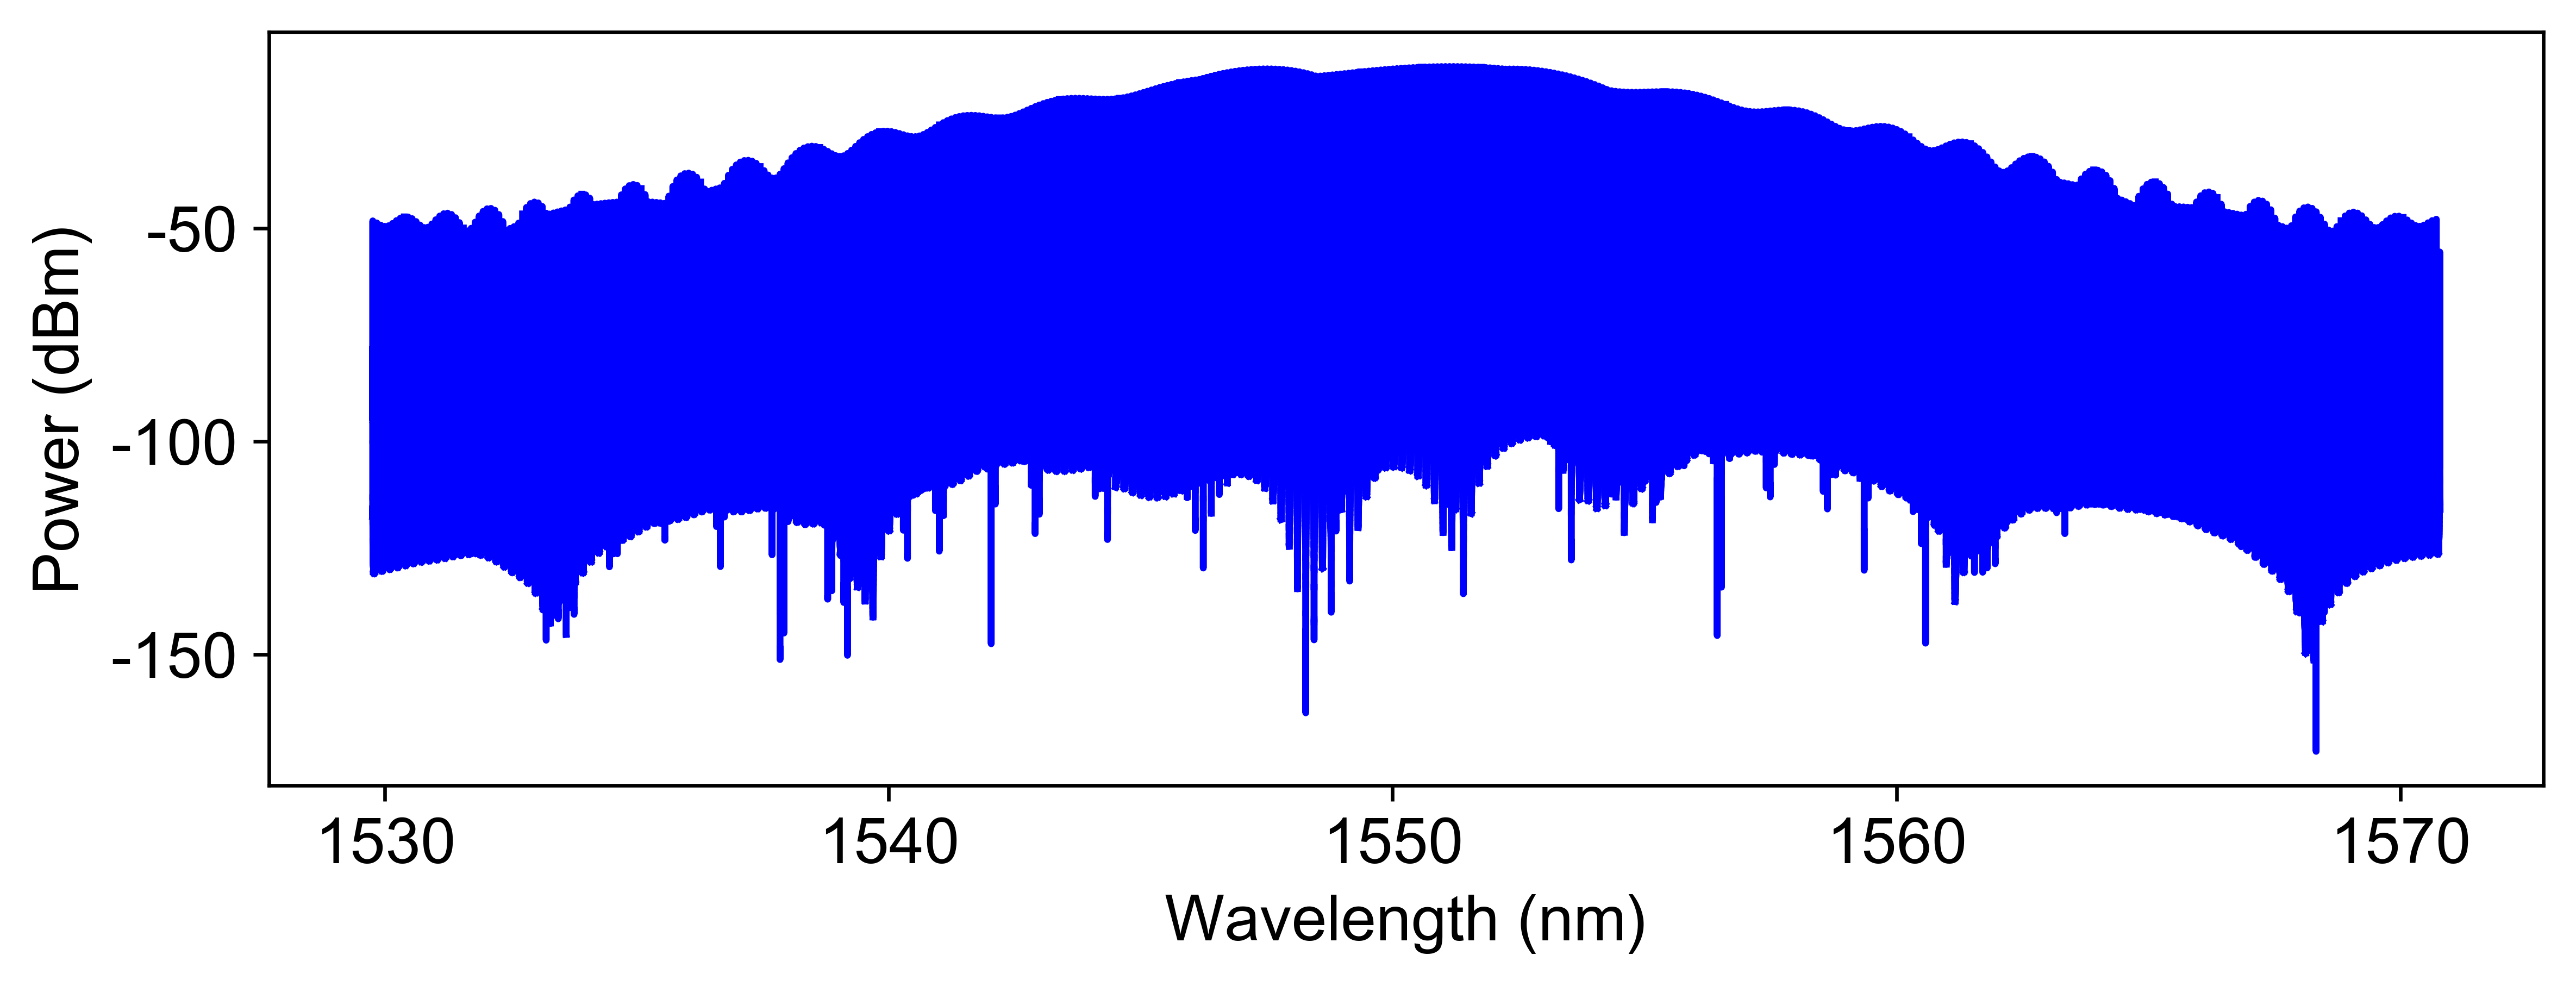
\includegraphics[width=0.48\linewidth]{figure/fig_21_0.png}
    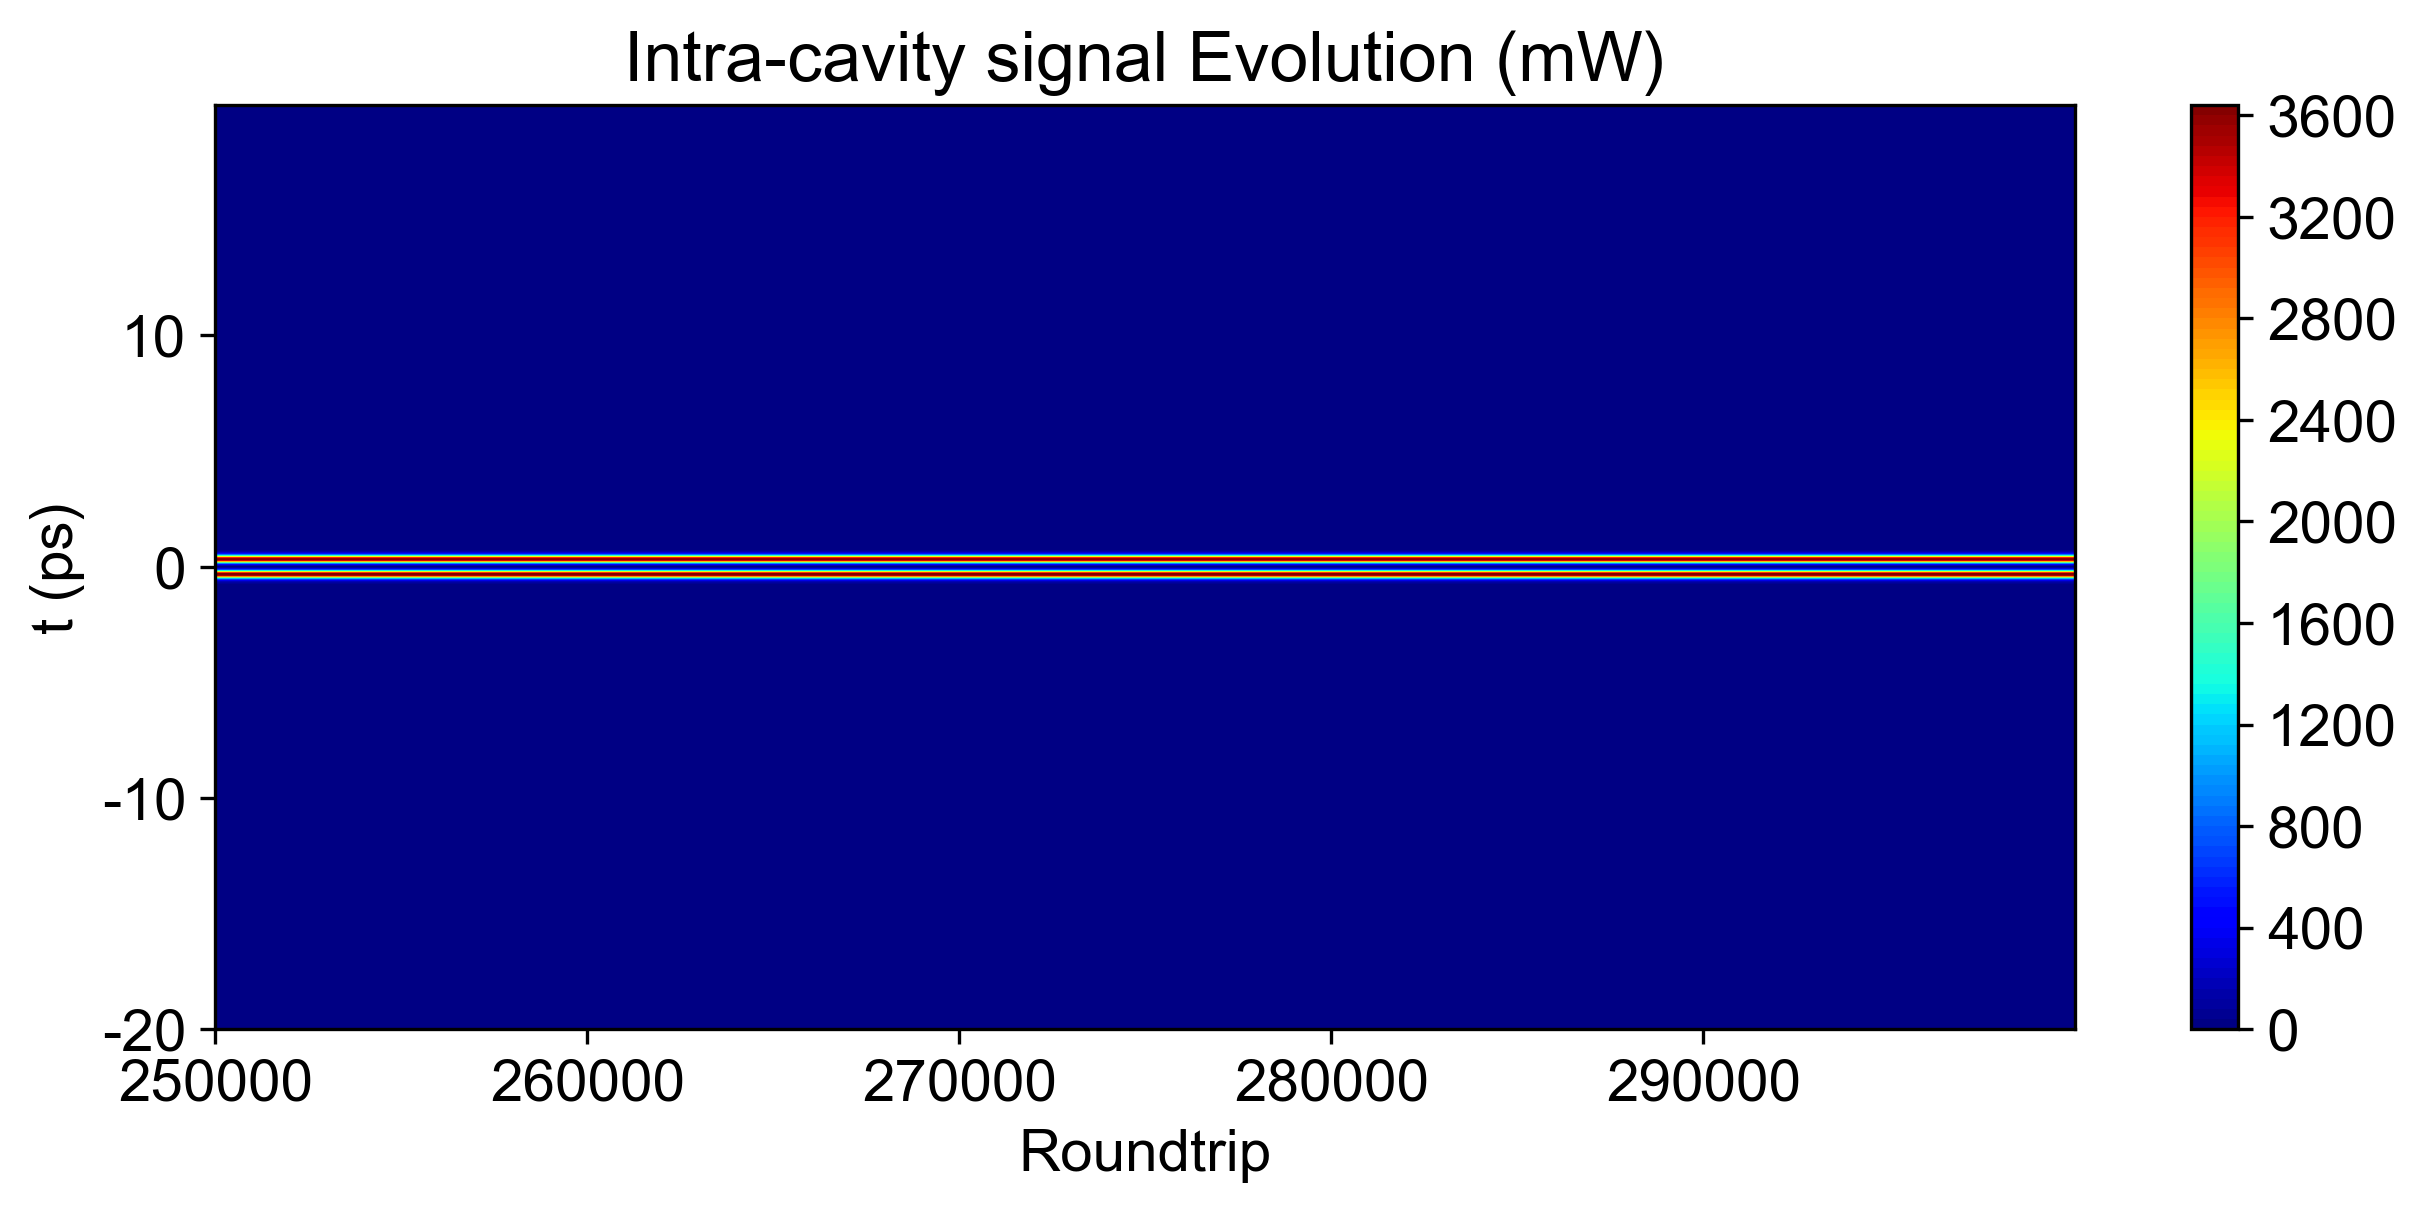
\includegraphics[width=0.48\linewidth]{figure/fig_22.png}
    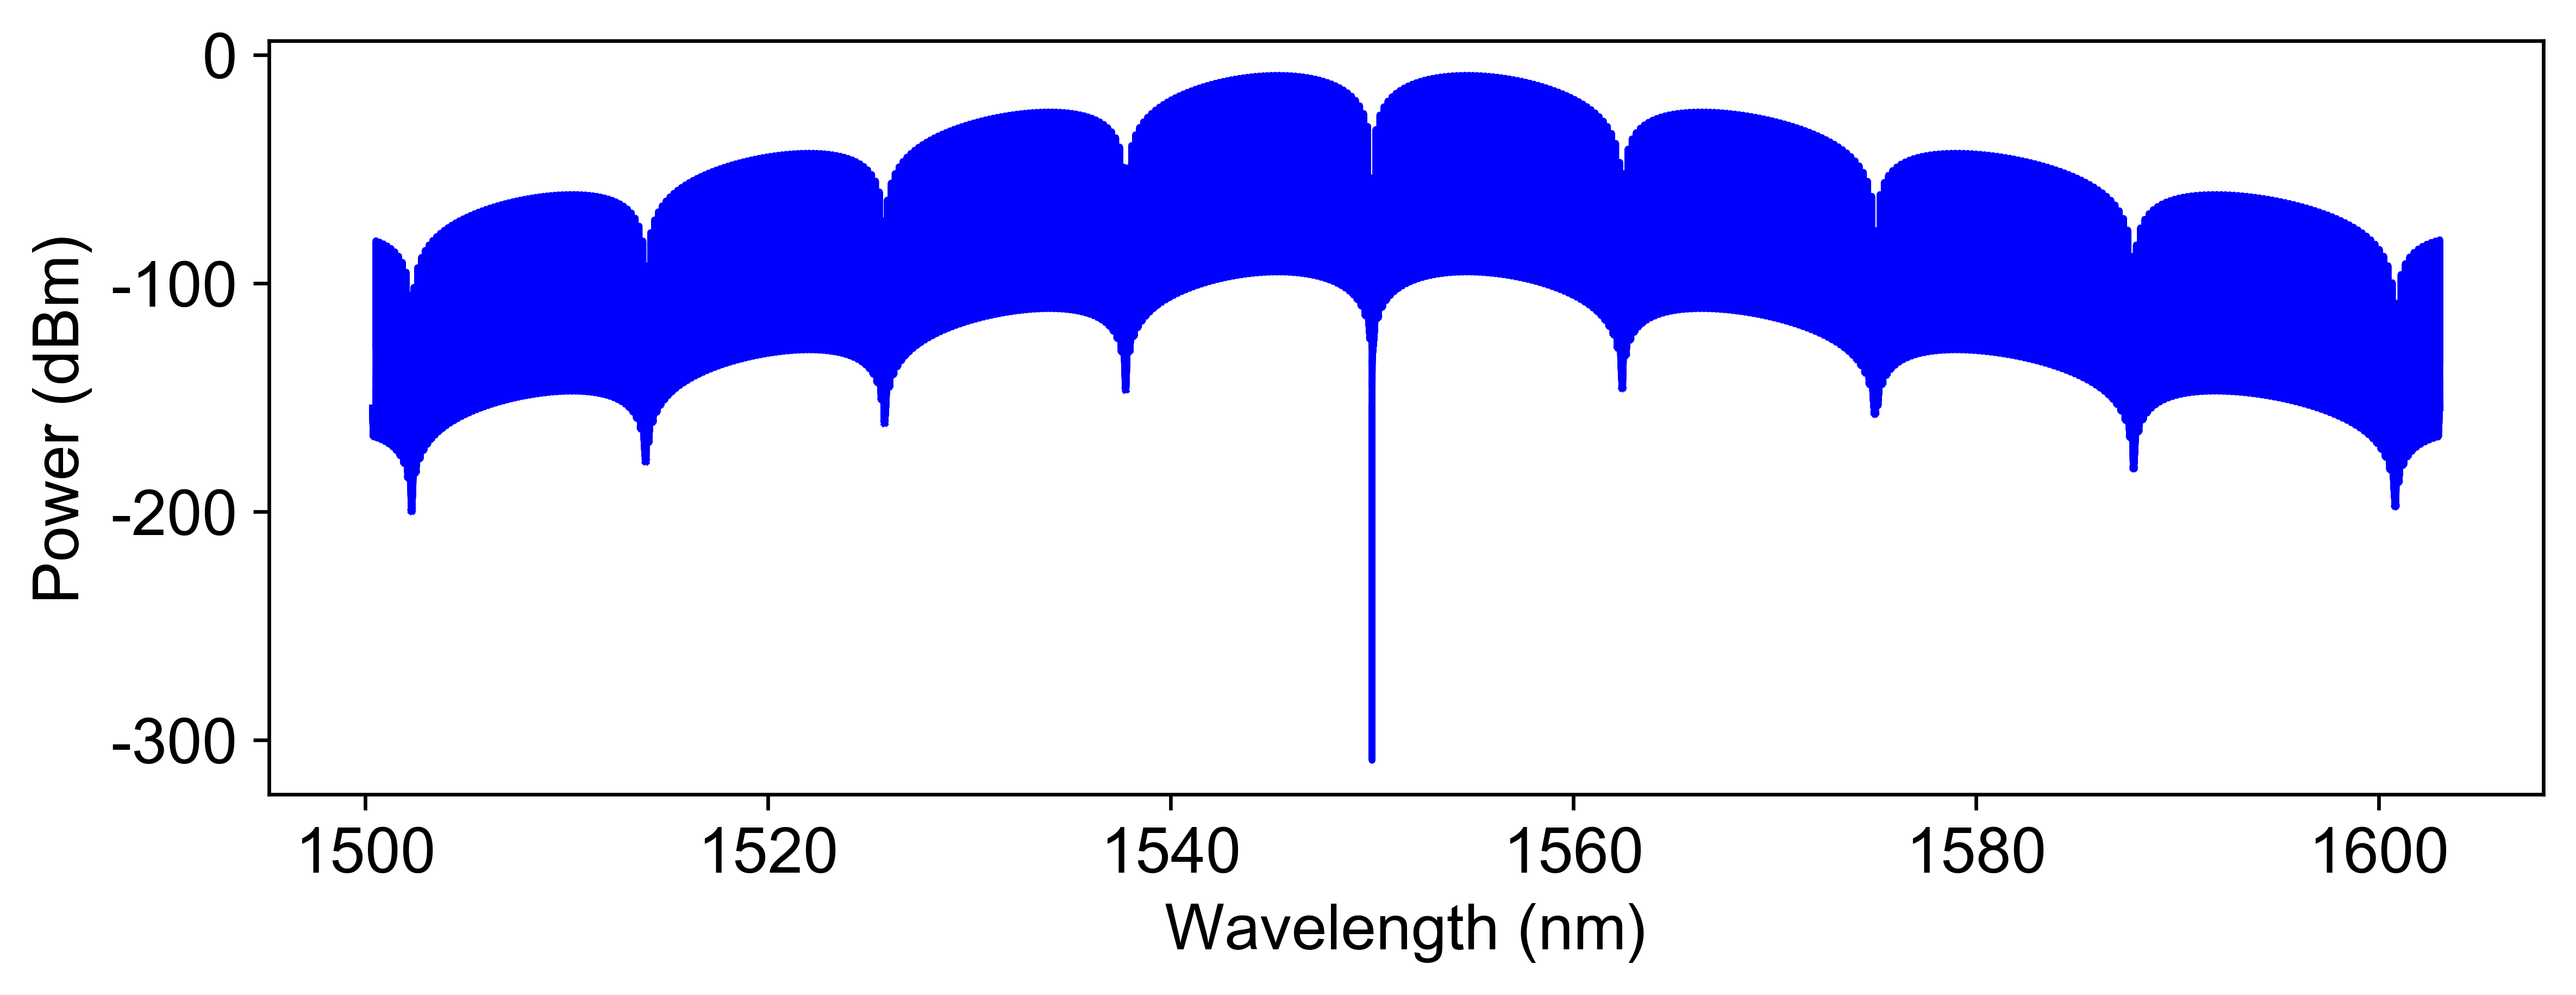
\includegraphics[width=0.48\linewidth]{figure/fig_22_0.png}
    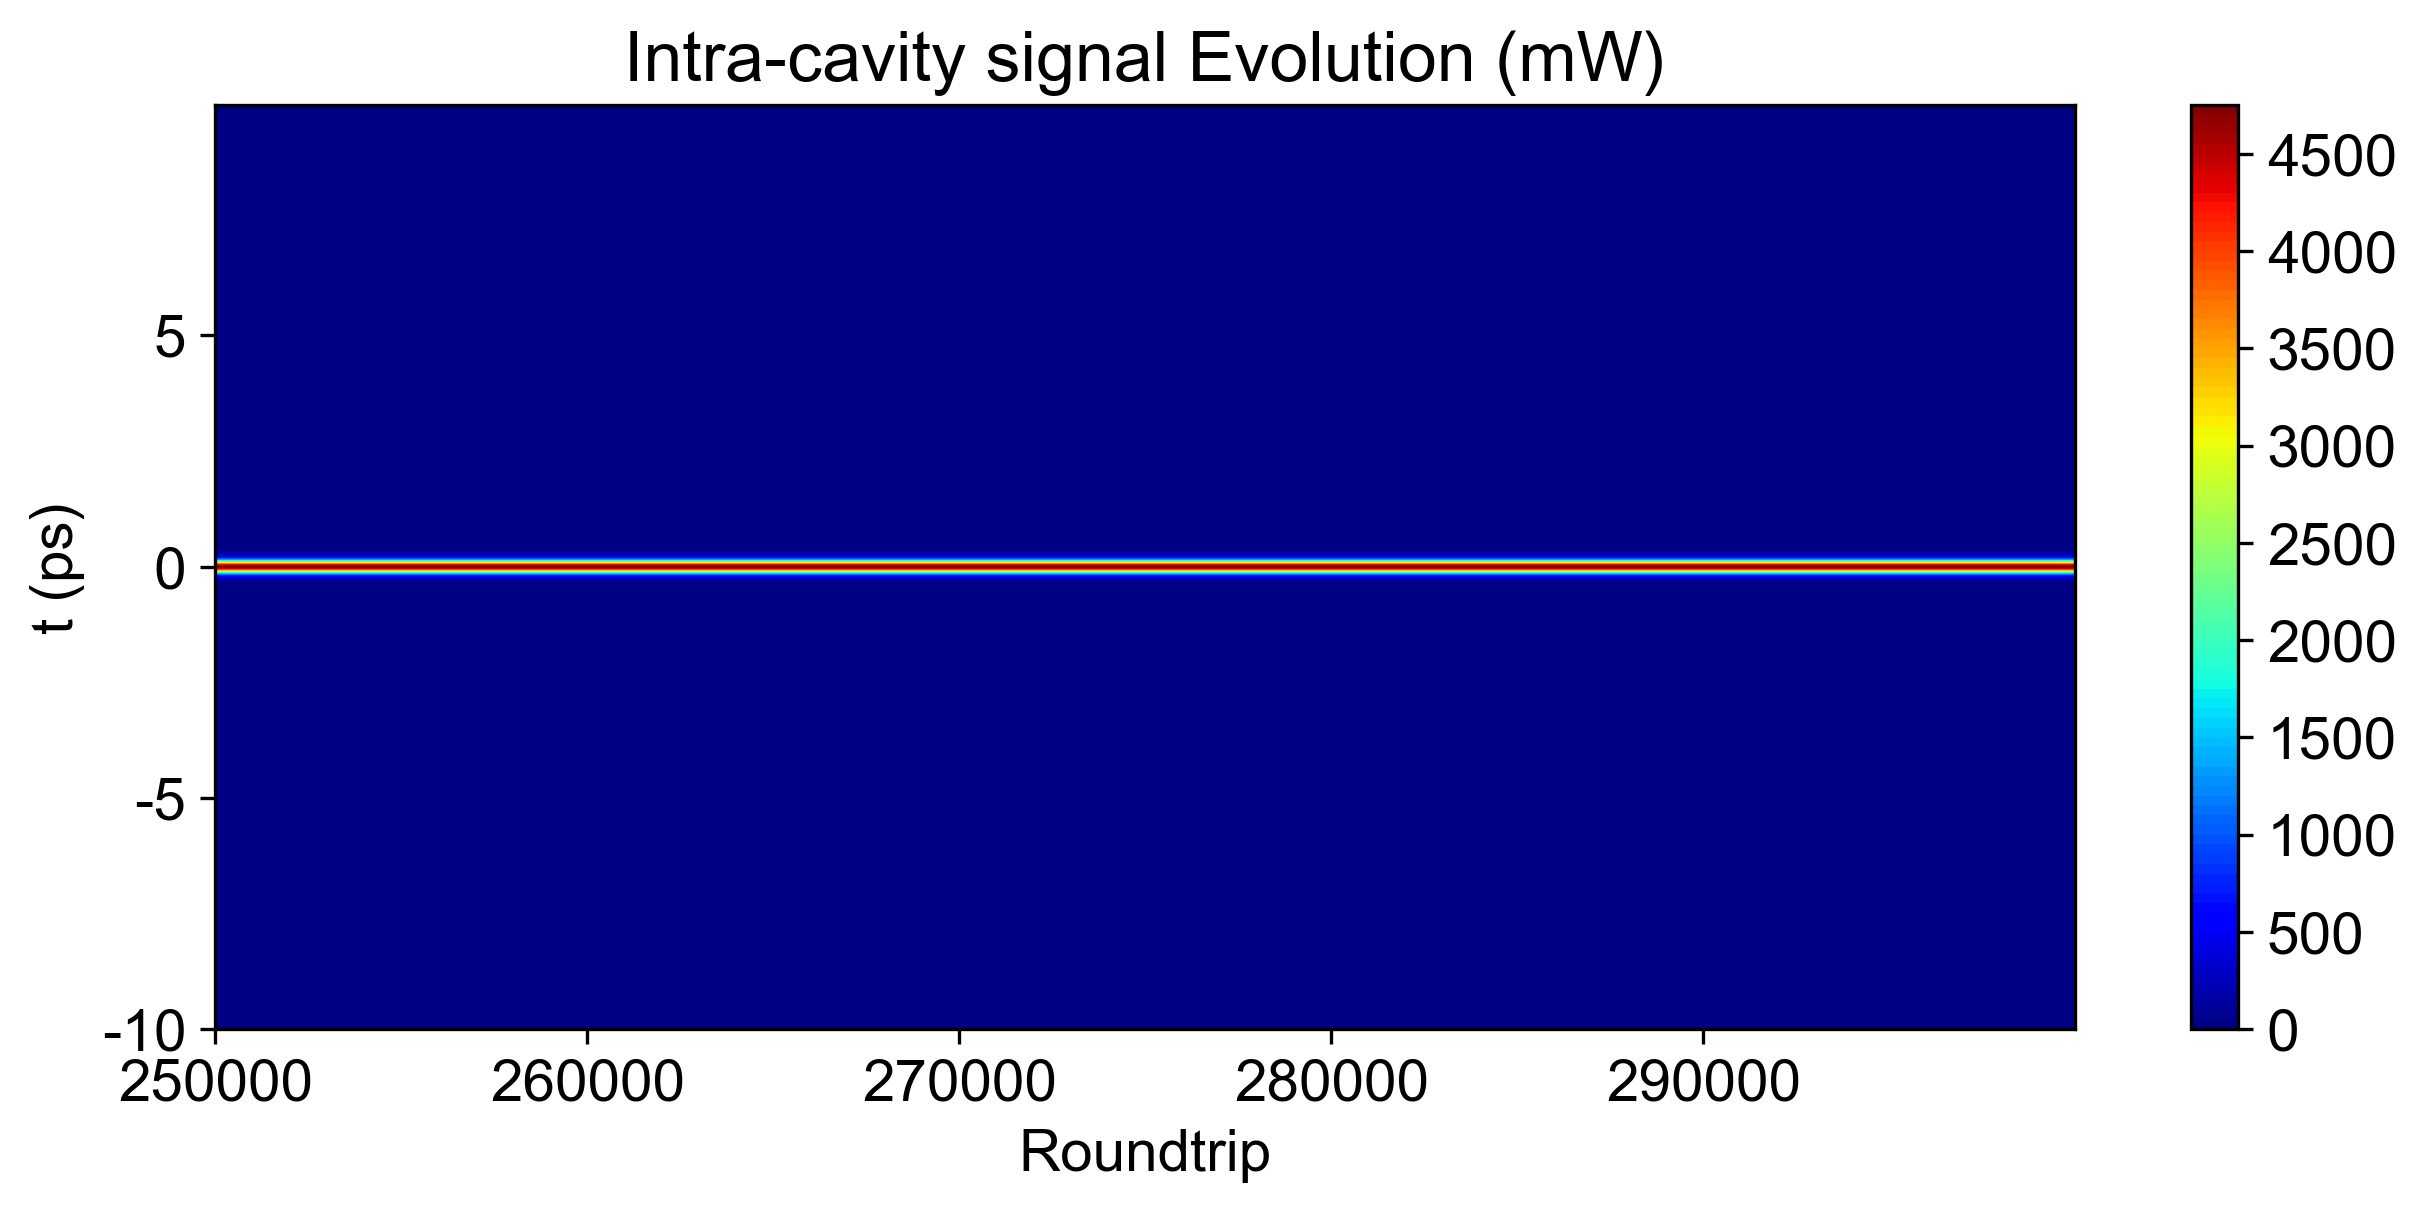
\includegraphics[width=0.48\linewidth]{figure/fig_23.png}
    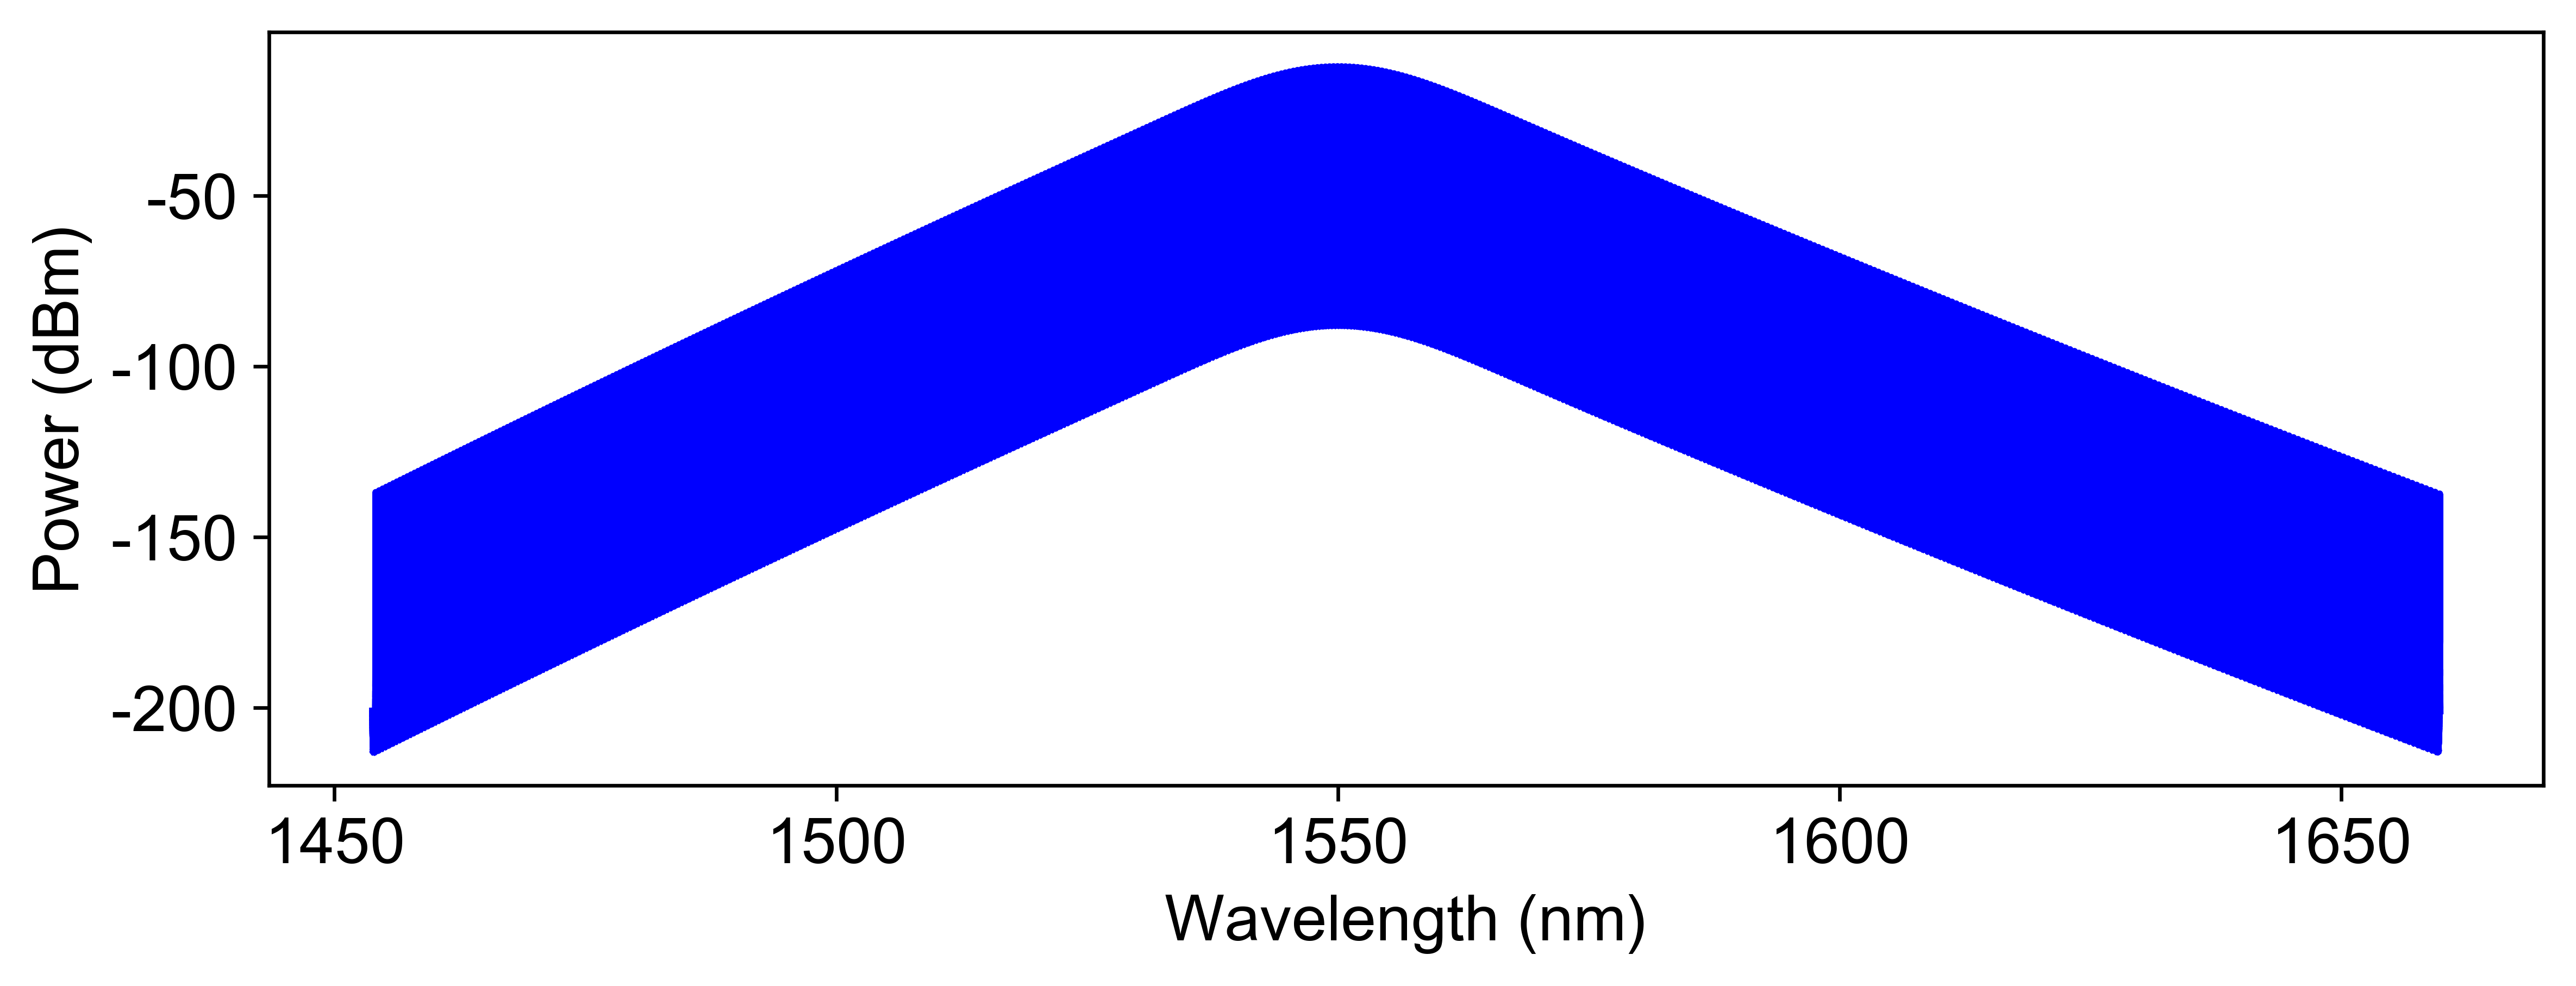
\includegraphics[width=0.48\linewidth]{figure/fig_23_0.png}
    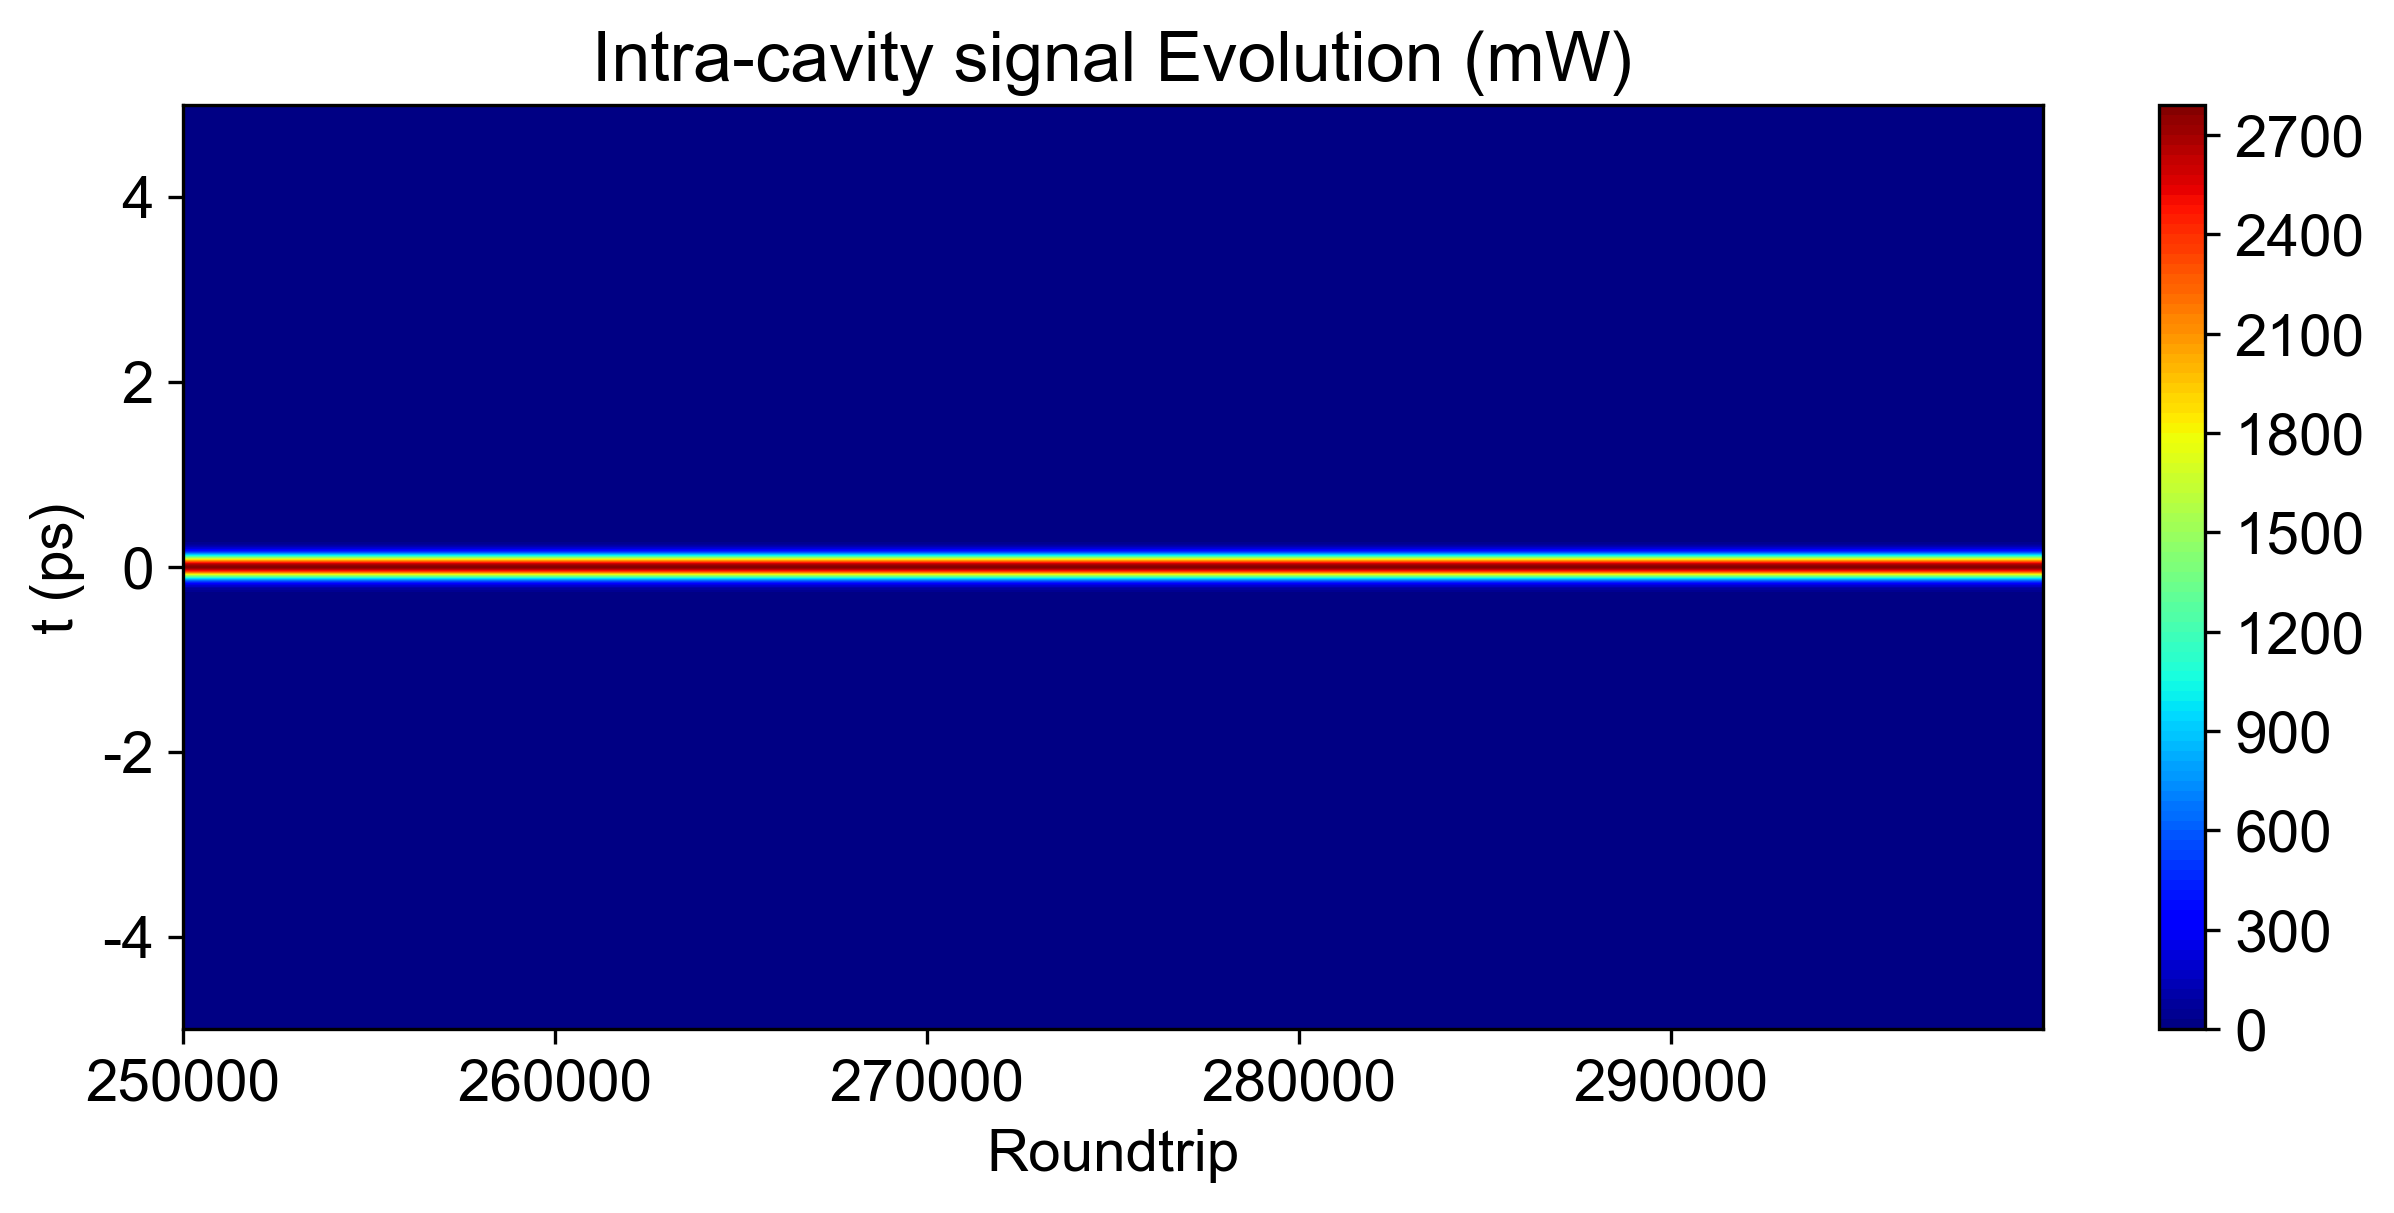
\includegraphics[width=0.48\linewidth]{figure/fig_24.png}
    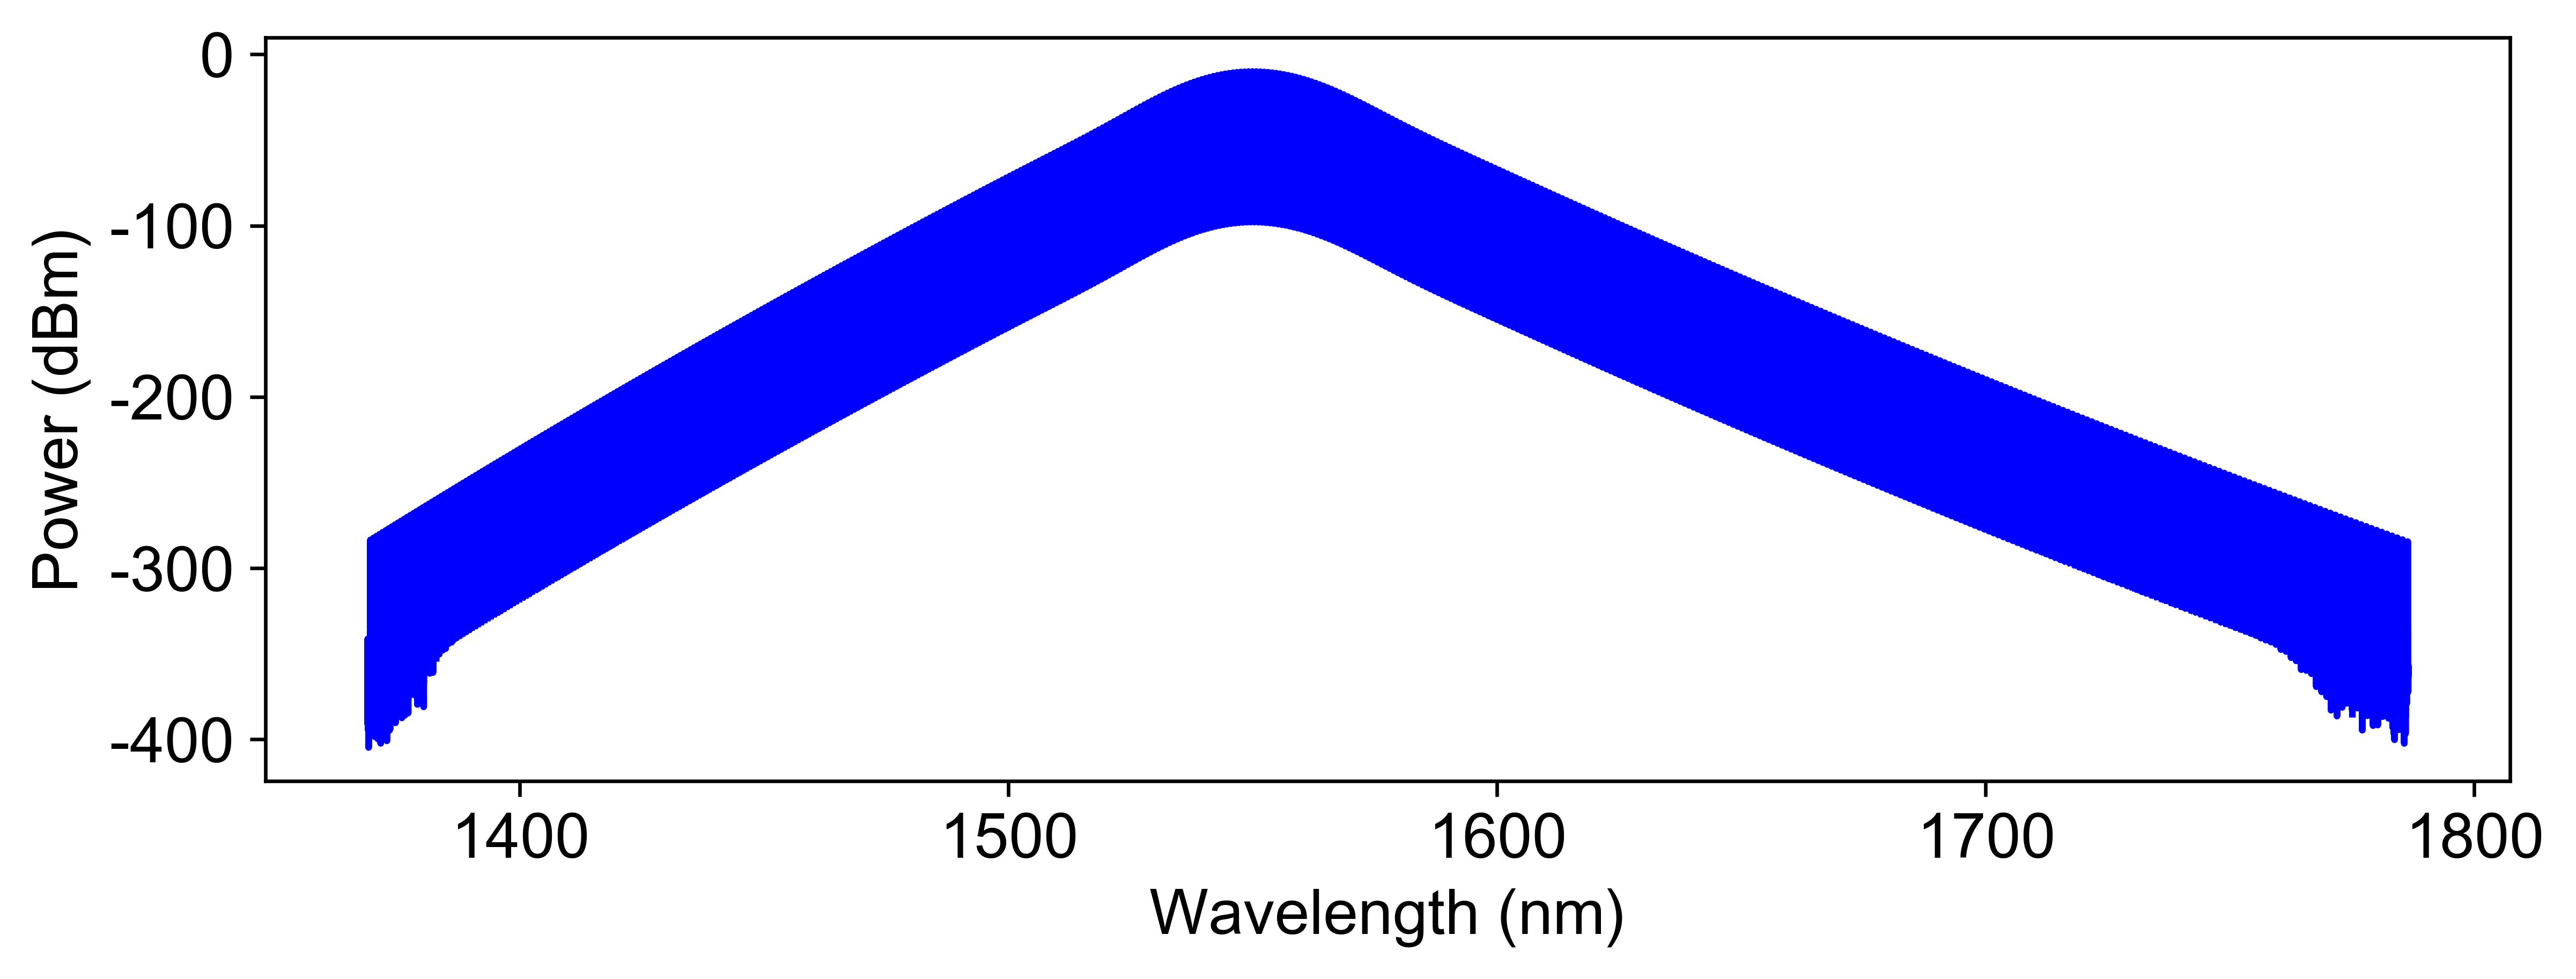
\includegraphics[width=0.48\linewidth]{figure/fig_24_0.png}
    \caption{左列:腔内信号光场的稳态,对应的光谱。从上到下$FSR$依次为:10,25,50,100GHz。}
    \label{fig:enter-label}
\end{figure}
$FSR$越大,越接近锁模态。
\section{泵浦转化效率}
% 只有在锁模的基础上讨论泵浦转化效率才有意义。\\
\begin{figure}[htbp]
    \centering
    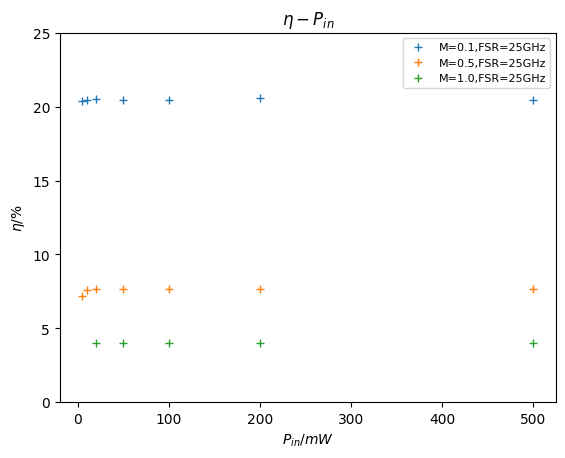
\includegraphics[width=0.99\linewidth]{figure/fig_25.png}
    \caption{不同调制深度下,泵浦转化效率和泵浦功率的关系图}
    \label{fig:enter-label}
\end{figure}
调制深度越大,泵浦光的耦合效率越低,因此转换效率越低。\\
泵浦功率变化时,增益介质的效率在饱和前都近似不变,锁模系统是线性的,不会饱和,因此转换效率近乎不变。\\
\section{本章小节}
调制深度,泵浦光功率,重频是影响锁模效果和泵浦转化效率的关键参数。本章通过数值仿真揭示了其定性关系。调制深度越大,锁模效果越好,但泵浦转化效率降低。重复频率越大,锁模效果越好,但泵浦转化效率降低。泵浦光功率越大,锁模效果越差,泵浦转化效率几乎不变,即输出功率正比于泵浦光功率。\\
本研究的目的是制造出重频在微波范围内、高转化效率、高功率的锁模激光器,但由于各参数的制约,三个条件不能同时满足。

	\chapter{总结和展望}

\fontsize{12bp}{14.4pt}

\section{总结}
本文通过数值模拟,验证了集成主动锁模激光器的可行性,给出了转换效率关于调制深度、泵浦功率、微腔重复频率的仿真结果和定性关系。\\
仿真发现,高输出功率和高转换效率相矛盾。可以理解为高输出功率需要高泵浦,进而需要更大的调制深度保持锁模,这就降低了泵浦耦合效率。\\
进一步的仿真证明,自发放大辐射对能否锁模不会造成决定性的影响。
\section{展望:锁模过程的研究}
除了高调制深度带来的单个脉冲,在临界条件附近还出现了双脉冲,振荡脉冲等现象,表示系统可能不止一个稳态。多稳态的存在可能使得单脉冲态难以进入,因此对其他稳态的研究可能会发现新的单脉冲态存在区间以及进入方式。


    \section{参考文献}
[1]Berkdemir, Cüneyt, and Sedat Özsoy. ‘An Investigation on the Temperature Dependence of the Relative Population Inversion and the Gain in EDFAs by the Modified Rate Equations’. Optics Communications 254, no. 4–6 (October 2005): 248–55.\\


[2]Buscaino, Brandon, Mian Zhang, Marko Loncar, and Joseph M. Kahn. ‘Design of Efficient Resonator-Enhanced Electro-Optic Frequency Comb Generators’. Journal of Lightwave Technology 38, no. 6 (15 March 2020): 1400–1413.\\


[3]Carmon, Tal, Lan Yang, and Kerry J. Vahala. ‘Dynamical Thermal Behavior and Thermal Self-Stability of Microcavities’. Optics Express 12, no. 20 (4 October 2004): 4742.\\


[4]Del’Haye, P., T. Herr, E. Gavartin, M. L. Gorodetsky, R. Holzwarth, and T. J. Kippenberg. ‘Octave Spanning Tunable Frequency Comb from a Microresonator’. Physical Review Letters 107, no. 6 (1 August 2011): 063901.\\


[5]Del’Haye, P., A. Schliesser, O. Arcizet, T. Wilken, R. Holzwarth, and T. J. Kippenberg. ‘Optical Frequency Comb Generation from a Monolithic Microresonator’. Nature 450, no. 7173 (December 2007): 1214–17. \\


[6]Diddams, Scott A., Kerry Vahala, and Thomas Udem. ‘Optical Frequency Combs: Coherently Uniting the Electromagnetic Spectrum’. Science 369, no. 6501 (17 July 2020): eaay3676. \\


[7]Englebert, Nicolas, Carlos Mas Arabí, Pedro Parra-Rivas, Simon-Pierre Gorza, and François Leo. ‘Temporal Solitons in a Coherently Driven Active Resonator’. Nature Photonics 15, no. 7 (July 2021): 536–41. \\


[8]Guo, H., M. Karpov, E. Lucas, A. Kordts, M.H.P. Pfeiffer, V. Brasch, G. Lihachev, V.E. Lobanov, M.L. Gorodetsky, and T.J. Kippenberg. ‘Universal Dynamics and Deterministic Switching of Dissipative Kerr Solitons in Optical Microresonators’. Nature Physics 13, no. 1 (January 2017): 94–102. \\


[9]He, Yang, Qi-Fan Yang, Jingwei Ling, Rui Luo, Hanxiao Liang, Mingxiao Li, Boqiang Shen, Heming Wang, Kerry Vahala, and Qiang Lin. ‘Self-Starting Bi-Chromatic LiNbO3 Soliton Microcomb’. Optica 6, no. 9 (20 September 2019): 1138–44. \\


[10]Herr, T., V. Brasch, J. D. Jost, C. Y. Wang, N. M. Kondratiev, M. L. Gorodetsky, and T. J. Kippenberg. ‘Temporal Solitons in Optical Microresonators’. Nature Photonics 8, no. 2 (February 2014): 145–52. \\


[11]Herr, T., K. Hartinger, J. Riemensberger, C. Y. Wang, E. Gavartin, R. Holzwarth, M. L. Gorodetsky, and T. J. Kippenberg. ‘Universal Formation Dynamics and Noise of Kerr-Frequency Combs in Microresonators’. Nature Photonics 6, no. 7 (July 2012): 480–87. \\


[12]Kippenberg, T. J., R. Holzwarth, and S. A. Diddams. ‘Microresonator-Based Optical Frequency Combs’. Science 332, no. 6029 (29 April 2011): 555–59. \\


[13]Liu, YiAn, XiongShuo Yan, JiangWei Wu, Bing Zhu, YuPing Chen, and XianFeng Chen. ‘On-Chip Erbium-Doped Lithium Niobate Microcavity Laser’. Science China Physics, Mechanics and Astronomy 64, no. 3 (March 2021): 234262. \\


[14]Vahala, Kerry J. ‘Optical Microcavities’. Nature 424, no. 6950 (August 2003): 839–46. \\


[15]Yi, Xu, Qi-Fan Yang, Ki Youl Yang, and Kerry Vahala. ‘Active Capture and Stabilization of Temporal Solitons in Microresonators’. Optics Letters 41, no. 9 (1 May 2016): 2037–40. \\


[16]Zhang, Mian, Brandon Buscaino, Cheng Wang, Amirhassan Shams-Ansari, Christian Reimer, Rongrong Zhu, Joseph M. Kahn, and Marko Lončar. ‘Broadband Electro-Optic Frequency Comb Generation in a Lithium Niobate Microring Resonator’. Nature 568, no. 7752 (April 2019): 373–77. \\


[17]Zhu, Di, Linbo Shao, Mengjie Yu, Rebecca Cheng, Boris Desiatov, C. J. Xin, Yaowen Hu, et al. ‘Integrated Photonics on Thin-Film Lithium Niobate’. Advances in Optics and Photonics 13, no. 2 (30 June 2021): 242–352. \\

    
    \appendix
    \printbibliography[heading = bibintoc]

	\backmatter
	% \chapter{致谢}

致谢部分...
	% 需添加二维码
	% % Copyright (c) 2008-2009 solvethis
% Copyright (c) 2010-2017,2021 Casper Ti. Vector
% Copyright (c) 2021 Kurapica
% Copyright (c) 2021 iofu728
% All rights reserved.
%
% Redistribution and use in source and binary forms, with or without
% modification, are permitted provided that the following conditions are
% met:
%
% * Redistributions of source code must retain the above copyright notice,
%   this list of conditions and the following disclaimer.
% * Redistributions in binary form must reproduce the above copyright
%   notice, this list of conditions and the following disclaimer in the
%   documentation and/or other materials provided with the distribution.
% * Neither the name of Peking University nor the names of its contributors
%   may be used to endorse or promote products derived from this software
%   without specific prior written permission.
%
% THIS SOFTWARE IS PROVIDED BY THE COPYRIGHT HOLDERS AND CONTRIBUTORS "AS
% IS" AND ANY EXPRESS OR IMPLIED WARRANTIES, INCLUDING, BUT NOT LIMITED TO,
% THE IMPLIED WARRANTIES OF MERCHANTABILITY AND FITNESS FOR A PARTICULAR
% PURPOSE ARE DISCLAIMED. IN NO EVENT SHALL THE COPYRIGHT HOLDER OR
% CONTRIBUTORS BE LIABLE FOR ANY DIRECT, INDIRECT, INCIDENTAL, SPECIAL,
% EXEMPLARY, OR CONSEQUENTIAL DAMAGES (INCLUDING, BUT NOT LIMITED TO,
% PROCUREMENT OF SUBSTITUTE GOODS OR SERVICES; LOSS OF USE, DATA, OR
% PROFITS; OR BUSINESS INTERRUPTION) HOWEVER CAUSED AND ON ANY THEORY OF
% LIABILITY, WHETHER IN CONTRACT, STRICT LIABILITY, OR TORT (INCLUDING
% NEGLIGENCE OR OTHERWISE) ARISING IN ANY WAY OUT OF THE USE OF THIS
% SOFTWARE, EVEN IF ADVISED OF THE POSSIBILITY OF SUCH DAMAGE.

{
	\ctexset{section = {
		format+ = {\centering}, beforeskip = {40bp}, afterskip = {15bp}
	}}
	\specialchap{北京大学学位论文原创性声明和使用授权说明}

	% 学校书面要求本页面不要页码,但在给出的 Word 模版中又有页码。
	% 此处以学校书面要求为准。
	\thispagestyle{empty}
	\mbox{}\vspace*{-3em}
	\section*{原创性声明}

	本人郑重声明:
	所呈交的学位论文,是本人在导师的指导下,独立进行研究工作所取得的成果。
	除文中已经注明引用的内容外,
	本论文不含任何其他个人或集体已经发表或撰写过的作品或成果。
	对本文的研究做出重要贡献的个人和集体,均已在文中以明确方式标明。
	本声明的法律结果由本人承担。
	\vskip 1em
	\rightline{%
		论文作者签名:\hspace{5em}%
		日期:\hspace{2em}年\hspace{2em}月\hspace{2em}日%
	}

	\section*{%
		学位论文使用授权说明\\[-0.33em]
		\textmd{\zihao{5}(必须装订在提交学校图书馆的印刷本)}%
	}

	本人完全了解北京大学关于收集、保存、使用学位论文的规定,即:
	\begin{itemize}
		\item 按照学校要求提交学位论文的印刷本和电子版本;
		\item 学校有权保存学位论文的印刷本和电子版,
			并提供目录检索与阅览服务,在校园网上提供服务;
		\item 学校可以采用影印、缩印、数字化或其它复制手段保存论文;
		\item 因某种特殊原因须要延迟发布学位论文电子版,
			授权学校在 $\Box$\nobreakspace{}一年 /
			$\Box$\nobreakspace{}两年 /
			$\Box$\nobreakspace{}三年以后在校园网上全文发布。
	\end{itemize}
	\centerline{(保密论文在解密后遵守此规定)}
	\vskip 1em
	\rightline{%
		论文作者签名:\hspace{5em}导师签名:\hspace{5em}%
		日期:\hspace{2em}年\hspace{2em}月\hspace{2em}日%
	}

    % 若须排版二维码,请将二维码图片重命名为“barcode”,
    % 二维码内容为: 北京大学 xx学院 xx专业 xxx
    % 容错设置25%
    % 转为合适的图片格式,并放在当前目录下,然后去掉下面 2 行的注释。
    % \vfill\noindent
    % \includegraphics[height = 5em]{barcode}
}

% vim:ts=4:sw=4



\end{document}

% vim:ts=4:sw=4
